\ifx\wholebook\relax \else

\documentclass[b5paper]{ctexart}
\usepackage[nomarginpar
  %, margin=.5in
]{geometry}

\addtolength{\oddsidemargin}{-0.05in}
\addtolength{\evensidemargin}{-0.05in}
\addtolength{\textwidth}{0.1in}

\usepackage[cn]{../prelude}

\setcounter{page}{1}

\begin{document}

\title{无理数}

\author{刘新宇
\thanks{{\bfseries 刘新宇} \newline
  Email: liuxinyu99@hotmail.com \newline}
  }

\maketitle
\fi

\markboth{无理数}{数的旅程}

\ifx\wholebook\relax
\chapter{无理数}
\fi

\epigraph{宇宙这本大书是用数学书写的}{伽利略}

公元前240年的夏至中午,这一天是一年中日照最长的一日,大约是现代历法的6月21日附近。埃及亚历山大港图书馆馆长埃拉托斯特尼(公元前276年~194年)正和一位来自赛印城的商人交谈。赛印(Syene)位于今天埃及南部的阿斯旺,是北回归线上的一个城市。“我的老家是世上最干最热的地方。”商人说道:“我们打了很深的井汲水,每年的这个时候,阳光能射到井底呢。”听到这句话时埃拉托斯特尼注意到了到广场上纪念碑的影子。为什么会这样呢?除非大地不是平坦的,而是球形。他询问哪个商人:“从赛印城到亚历山大有多远的路程?”“有5000斯塔蒂亚。”斯塔蒂亚(Stadia)是古希腊的长度单位,约和158米。埃拉托色特尼测量了立在地上的杆子和影子的长度,发现杆子的长度大约是影子长度的8倍。他于是按照\cref{fig:eratosthenes-earth}进行了计算。

\begin{figure}[htbp]
 \centering
 \subcaptionbox{太阳在夏至直射北回归线上的赛印城\label{fig:eratosthenes-earth}}{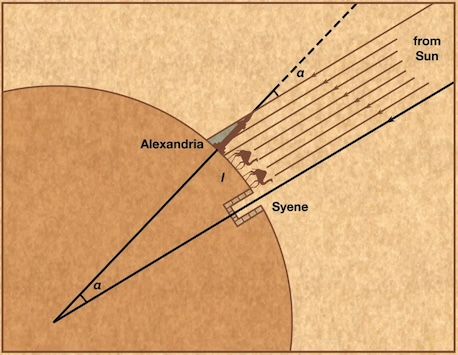
\includegraphics[scale=0.35]{img/eratosthenes-earth}}
 \subcaptionbox{太阳照射亚历山大的角度为$\alpha$\label{fig:atan8}}{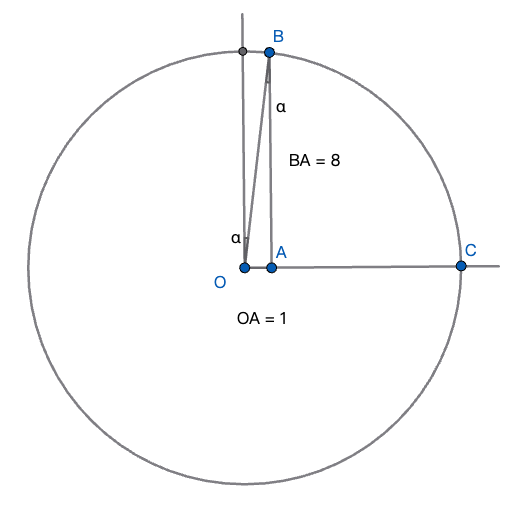
\includegraphics[scale=0.32]{img/atan8}}
 \caption{埃拉托斯特尼测量地球}
\end{figure}

夏至正午时刻,太阳直射北回归线,因此阳光可以射入赛印城的井底。埃拉托色特尼可以通过\cref{fig:atan8}找出阳光照射亚历山大港的角度。
%% 这相当于今天高中数学中的反正切$\arctan(\frac{1}{8})$。
但当时古巴比伦的角度单位还没有传入古希腊,按照埃拉托斯特尼的说法,这个角度是圆的50分之一,合$7.2\degree$。太阳光是平行光。如果大地是球形的,那么赛印城和亚历山大到球心的张角,是太阳入射角的同位角(\cref{fig:eratosthenes-earth}中标有$\alpha$的两个角),也是圆的50分之一。所以赛印城到亚历山大之间的距离就是地球周长的50分之一。这样算来,地球的周长就是$50 \times 5000 = 250000$斯塔提雅,约合$250 \times 158 = 39500 \approx 4$万千米。而今天人们通过人造卫星测得地球赤道长度为40075千米。埃拉托色特尼的著作没有流传到今天,我们从古希腊数学家帕普斯等人的记述中了解到他的具体测量方法。埃拉托色特尼约在公元前235年起任亚历山大图书馆馆长,他对地球的测量发生在这一时期\cite{Walkup2005}。赛印城到亚历山大的距离是一个关键,5000斯塔蒂亚无疑是一个大致数字。埃拉托斯特尼可能通过多种途径核证该距离,包括询问往来的商人以及测量地图。赛印城和亚历山大港都是尼罗河沿岸城市,尼罗河有规律的每年泛滥,埃及人因此每年在泛滥后重新丈量尼罗河沿线的土地并更新地图。此外,古希腊的斯塔蒂亚到底有多长学者们也有不同的观点。无论如何,埃拉托色特尼在2000年前的伟大推理和计算无疑是惊人的。

\begin{figure}[htbp]
 \centering
 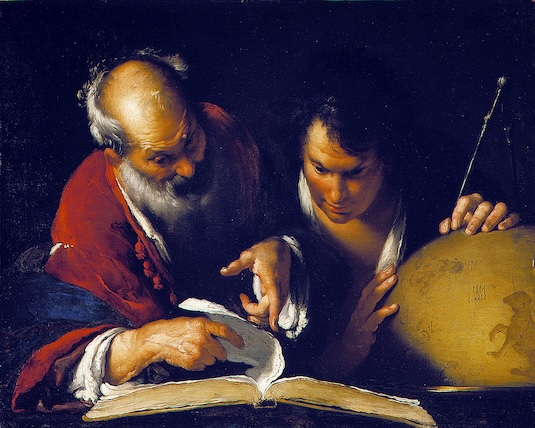
\includegraphics[scale=0.35]{img/eratosthenes}
 % https://commons.wikimedia.org/wiki/File:Eratosthenes_Teaching_in_Alexandria_(Bernardo_Strozzi,_Montreal).jpg
 \caption{贝尔纳多·斯特罗齐于1635年创作的油画:在亚历山大教学的埃拉托色特尼}
 \label{fig:eratosthenes}
\end{figure}

马其顿国王亚历山大大帝征服埃及后,兴建了以他命名的城市亚历山大港,成为了希腊化时代的文化和学术中心。埃拉托色特尼测量地球的壮举通常被认为是体现古希腊几何学力量的典范。古希腊并没有位值制计数系统(见第1章),但却发展出了严密的推理和几何学传统。正是在把数和几何学结合后,古希腊人\underdot{发现}了无理数,使得数的大家庭又得到了一次扩充。

\section{万物皆数}
音乐与数似乎毫无关联,但毕达哥拉斯却发现了它们背后竟有奇妙的规律。他从中得到启发并大胆推测“万物皆数”(All is number),认为世间万物都可以用数或数的比例来理解。毕达哥拉斯可以说是用数探索世间万物的第一人。他出生于希腊的萨摩斯(Samos)岛,年轻时他曾去米利都(Miletus)向古希腊哲学的奠基人泰勒斯(Thales)学习。在泰勒斯的建议下,毕达哥拉斯于公元535年前往埃及学习数学。公元前525年,波斯帝国征服了埃及,他被俘并随军向东到达了巴比伦。毕达哥拉斯得以向巴比伦人学习数学和天文知识。或许后来他还到达了更远的印度。不论到了哪里,毕达哥拉斯都不断向有学问的人请教,丰富自己的见解。重要的是,他不仅刻苦学习,而且更善于思考。在经过兼收并蓄、汲取各家之长后,毕达哥拉斯形成并完善了自己的思想\cite{HanXueTao16}。

经历了漫长的在外游历后,年近半百的毕达哥拉斯返回了故乡萨默斯并开始讲学。公元前520年左右,也许为了摆脱当地的暴政,毕达哥拉斯移居到了意大利南部的克罗顿(Croton)发展。在那里他赢得了人们的信任与景仰并形成了自己的学派。毕达哥拉斯的弟子中还有女性,学派把主要精力都用来研究天文、几何、数论、音乐这四门学科。它们被称为四术(quadrivium),影响了欧洲教育两千多年\cite{StepanovRose15}。四术体现了毕达哥拉斯万物皆数的哲学思想:星体的运动与几何对应,而几何又以数为基础,数字还可以衍生出音乐(见第3章)。关于毕达哥拉斯去世有多种说法。他领导的学派具有很高的声誉和政治影响,引起了敌对派的忌恨。约公元前497年,学派在克罗顿的活动场所遭到破坏。有人认为毕达哥拉斯被暴徒杀害,也有人说他逃到梅塔蓬图姆(Metapontum)并度过余生\cite{MKlein1972}。

\index{形数(figurate number)}
毕达哥拉斯学派研究数字,认为数与数、数与自然之间存在着神秘关系。这开启了数学的重要分支——数论。学派对正整数进行了分类,定义了奇数、偶数、素数、合数等。他们通过在地上摆小石子来研究数字,英文的计算calculus一词就是从希腊文“石子”衍生出的\cite{HanXueTao16}。当把石子按照某种几何图形摆放时,就得到了形数(figurate number)。

\begin{figure}[htbp]
%\begin{wrapfigure}{R}{0.4\textwidth}
\centering
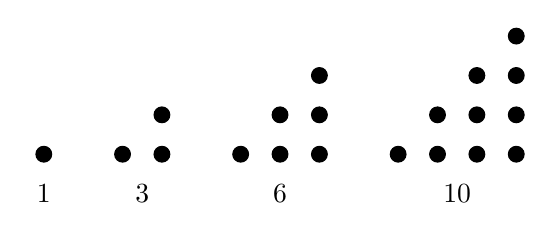
\begin{tikzpicture}[scale=0.5]
\filldraw (0, 0) circle (0.2);
\draw (0, -1) node{1};
\filldraw (2, 0) circle (0.2)
          (3, 0) circle (0.2)   (3, 1) circle (0.2);
\draw (2.5, -1) node{3};
\filldraw (5, 0) circle (0.2)
          (6, 0) circle (0.2)   (6, 1) circle (0.2)
          (7, 0) circle (0.2)   (7, 1) circle (0.2)   (7, 2) circle (0.2);
\draw (6, -1) node{6};
\filldraw (9, 0) circle (0.2)
          (10, 0) circle (0.2)    (10, 1) circle (0.2)
          (11, 0) circle (0.2)    (11, 1) circle (0.2)    (11, 2) circle (0.2)
          (12, 0) circle (0.2)    (12, 1) circle (0.2)    (12, 2) circle (0.2)    (12, 3) circle (0.2);
\draw (10.5, -1) node{10};
\end{tikzpicture}
\caption{三角形数(triangular number)}
\label{fig:triangular-num}
%\end{wrapfigure}
\end{figure}

\begin{figure}[htbp]
%\begin{wrapfigure}{R}{0.4\textwidth}
\centering
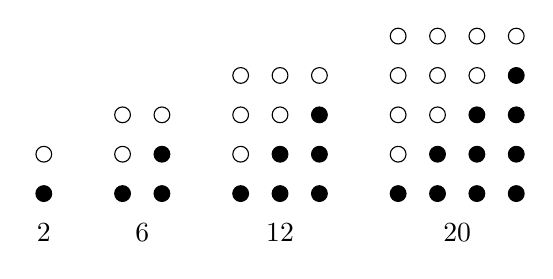
\begin{tikzpicture}[scale=0.5]
\draw (0, 1) circle (0.2);
\filldraw (0, 0) circle (0.2);
\draw (0, -1) node{2};

\draw (2, 1) circle (0.2)   (2, 2) circle (0.2)
      (3, 2) circle (0.2);
\filldraw (2, 0) circle (0.2)
          (3, 0) circle (0.2)   (3, 1) circle (0.2);
\draw (2.5, -1) node{6};

\draw (5, 1) circle (0.2)   (5, 2) circle (0.2)   (5, 3) circle (0.2)
      (6, 2) circle (0.2)   (6, 3) circle (0.2)
      (7, 3) circle (0.2);
\filldraw (5, 0) circle (0.2)
          (6, 0) circle (0.2)   (6, 1) circle (0.2)
          (7, 0) circle (0.2)   (7, 1) circle (0.2)   (7, 2) circle (0.2);
\draw (6, -1) node{12};

\draw (9, 1) circle (0.2)   (9, 2) circle (0.2)   (9, 3) circle (0.2)   (9, 4) circle (0.2)
      (10, 2) circle (0.2)   (10, 3) circle (0.2)   (10, 4) circle (0.2)
      (11, 3) circle (0.2)   (11, 4) circle (0.2)
      (12, 4) circle (0.2);
\filldraw (9, 0) circle (0.2)
          (10, 0) circle (0.2)    (10, 1) circle (0.2)
          (11, 0) circle (0.2)    (11, 1) circle (0.2)    (11, 2) circle (0.2)
          (12, 0) circle (0.2)    (12, 1) circle (0.2)    (12, 2) circle (0.2)    (12, 3) circle (0.2);
\draw (10.5, -1) node{20};
\end{tikzpicture}
\caption{长方形数(oblong number)}
\label{fig:oblong-num}
%\end{wrapfigure}
\end{figure}

\cref{fig:triangular-num}和\cref{fig:oblong-num}分别是三角形数和长方形数。容易看出,每个长方形数都对应三角形数的二倍,而三角形数又是前$n$个正整数之和,这样就得到了正整数累加的求和公式:

\[
1 + 2 + 3 + ... + n = \frac{1}{2}n(n+1)
\]

毕达哥拉斯学派还观察到,所有的奇数可以表示成折尺形(或称为“磬折形”)\footnote{gnomon这个字在巴比伦人的原意可能是指日晷上的直杆,用它的阴影来指示时刻。在毕达哥拉斯时代,gnomon指木匠用的方尺。它还表示从正方形的一角切掉一个小正方形后剩余的图形。以后欧几里得又把正方形扩展到平行四边形\citepage[26页]{MKlein1972}。},如\cref{fig:gnomon-num},而前$n$个折尺形可以拼成一个正方形,如\cref{fig:square-num}。这样他们就发现了前$n$个正奇数的求和公式:

\[
1 + 3 + 5 + ... + (2n - 1) = n^2
\]

\begin{figure}[htbp]
%\begin{wrapfigure}{R}{0.4\textwidth}
\centering
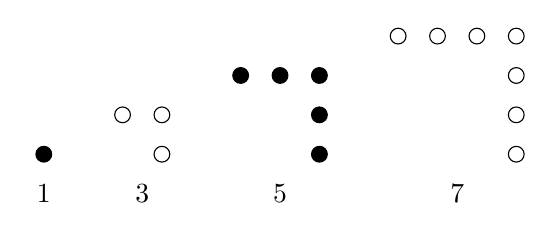
\begin{tikzpicture}[scale=0.5]
\filldraw (0, 0) circle (0.2);
\draw (0, -1) node{1};

\draw (2, 1) circle (0.2)
      (3, 0) circle (0.2)   (3, 1) circle (0.2);
\draw (2.5, -1) node{3};

\filldraw (5, 2) circle (0.2)   (6, 2) circle (0.2)   (7, 2) circle (0.2)
          (7, 0) circle (0.2)   (7, 1) circle (0.2);
\draw (6, -1) node{5};

\draw (9, 3) circle (0.2)   (10, 3) circle (0.2)   (11, 3) circle (0.2)   (12, 3) circle (0.2)
      (12, 0) circle (0.2)    (12, 1) circle (0.2)    (12, 2) circle (0.2);
\draw (10.5, -1) node{7};
\end{tikzpicture}
\caption{折尺形数(gnomon number)}
\label{fig:gnomon-num}
%\end{wrapfigure}
\end{figure}

\begin{figure}[htbp]
%\begin{wrapfigure}{R}{0.4\textwidth}
\centering
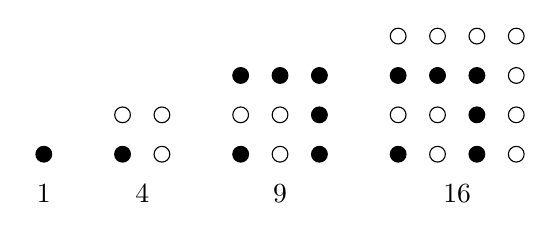
\begin{tikzpicture}[scale=0.5]
\filldraw (0, 0) circle (0.2);
\draw (0, -1) node{1};

\filldraw (2, 0) circle (0.2);
\draw (2, 1) circle (0.2)
      (3, 0) circle (0.2)   (3, 1) circle (0.2);
\draw (2.5, -1) node{4};

\filldraw (5, 0) circle (0.2);
\draw (5, 1) circle (0.2)
      (6, 0) circle (0.2)   (6, 1) circle (0.2);
\filldraw (5, 2) circle (0.2)   (6, 2) circle (0.2)   (7, 2) circle (0.2)
          (7, 0) circle (0.2)   (7, 1) circle (0.2);
\draw (6, -1) node{9};

\filldraw (9, 0) circle (0.2);
\draw (9, 1) circle (0.2)
      (10, 0) circle (0.2)   (10, 1) circle (0.2);
\filldraw (9, 2) circle (0.2)   (10, 2) circle (0.2)   (11, 2) circle (0.2)
          (11, 0) circle (0.2)   (11, 1) circle (0.2);
\draw (9, 3) circle (0.2)   (10, 3) circle (0.2)   (11, 3) circle (0.2)   (12, 3) circle (0.2)
      (12, 0) circle (0.2)    (12, 1) circle (0.2)    (12, 2) circle (0.2);
\draw (10.5, -1) node{16};
\end{tikzpicture}
\caption{正方形数(square number)与折尺形数的关系}
\label{fig:square-num}
%\end{wrapfigure}
\end{figure}

就这样,毕达哥拉斯学派把几何形状也建立在了数的基础上。他们热衷与用数去解释更多的现象,并相信宇宙的本质就在于“数的和谐”,由此出发,毕达哥拉斯学派试图发展一套以数字为基础的理论,使得几何学可以建立在该理论之上。

\section{勾股定理}

\begin{figure}[htbp]
 \centering
 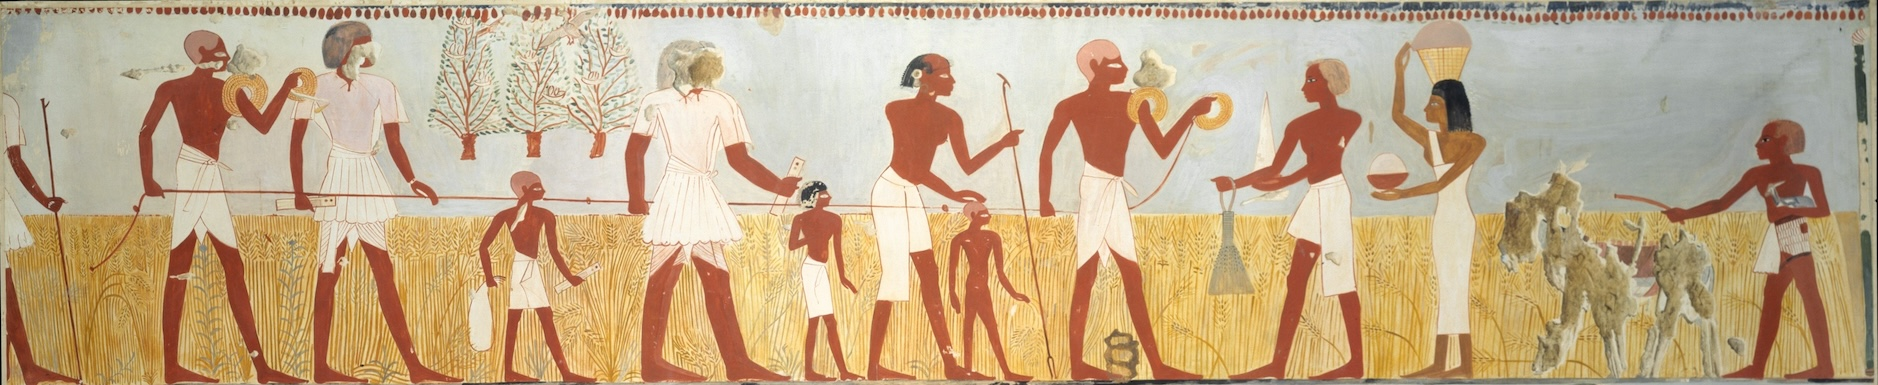
\includegraphics[scale=0.35]{img/harvest-scene}
 \caption{拉绳测量,来自梅纳陵墓壁画《收割场景》上半部分。梅纳是古埃及第十八王朝(公元前1400~1352年)的祭司和土地丈量官。现收藏于美国大都会艺术博物馆。}
 %% https://www.metmuseum.org/art/collection/search/548574
 \label{fig:rope-meter}
\end{figure}

毕达哥拉斯学派最著名的发现当属勾股定理,在西方叫做“毕达哥拉斯定理”。据说毕达哥拉斯对他发现的这个定理及其证明极为高兴,为此献祭了一百头公牛庆贺。但脍炙人口的传说故事往往不真实。毕达哥拉斯学派对团体成员有着极为严格的戒律,任何人的研究发现都归学派所有并必须保密。我们所知的以“毕达哥拉斯”命名的成果大都来自学派内的佚名作者。勾股定理并非孤立成果,各个文明都各自独立发现了它。如第3章中的\cref{fig:babylonian-yale}所示,这块古巴比伦泥板的时间大约是公元前1900年~1600年,此外人们还发现了刻有勾股数表的泥板。古埃及的测量员绳子作为软尺(称为拉绳人,见\cref{fig:rope-meter})。相传他们在绳上打结,把全长分成长度为3比4比5的三段,然后用来形成直角三角形。但这个说法没有文献证实\citepage[16页]{MKlein1972}。古印度数学家包德哈亚那(Baudhayana,生活在公元前800年到公元前400年间)的著作《绳法经》(Śulba Sutra)也提到了这个定理。在古代中国,成书于公元前一世纪的《周髀算经》中载有西周时代(约公元前11世纪)周公和商高的一段对话,其中提到“勾三、股四、弦五”\footnote{商高说:“……故折矩,勾广三,股修四,经隅五。”},故在中国称之为“勾股定理”。《九章算术》的注解中载有三国时代的赵爽和魏晋时刘徽给出的勾股定理证明\footnote{对赵爽和刘徽给出的究竟是严格意义的证明还是某种程度的解释历来有不同观点。}。

\begin{figure}[htbp]
 \centering
 \subcaptionbox{中国数学会会徽\label{fig:cms-logo}}{
\includegraphics[scale=0.5]{img/cms}} \quad
 \subcaptionbox{赵爽弦图\label{fig:zhaoshuang}}{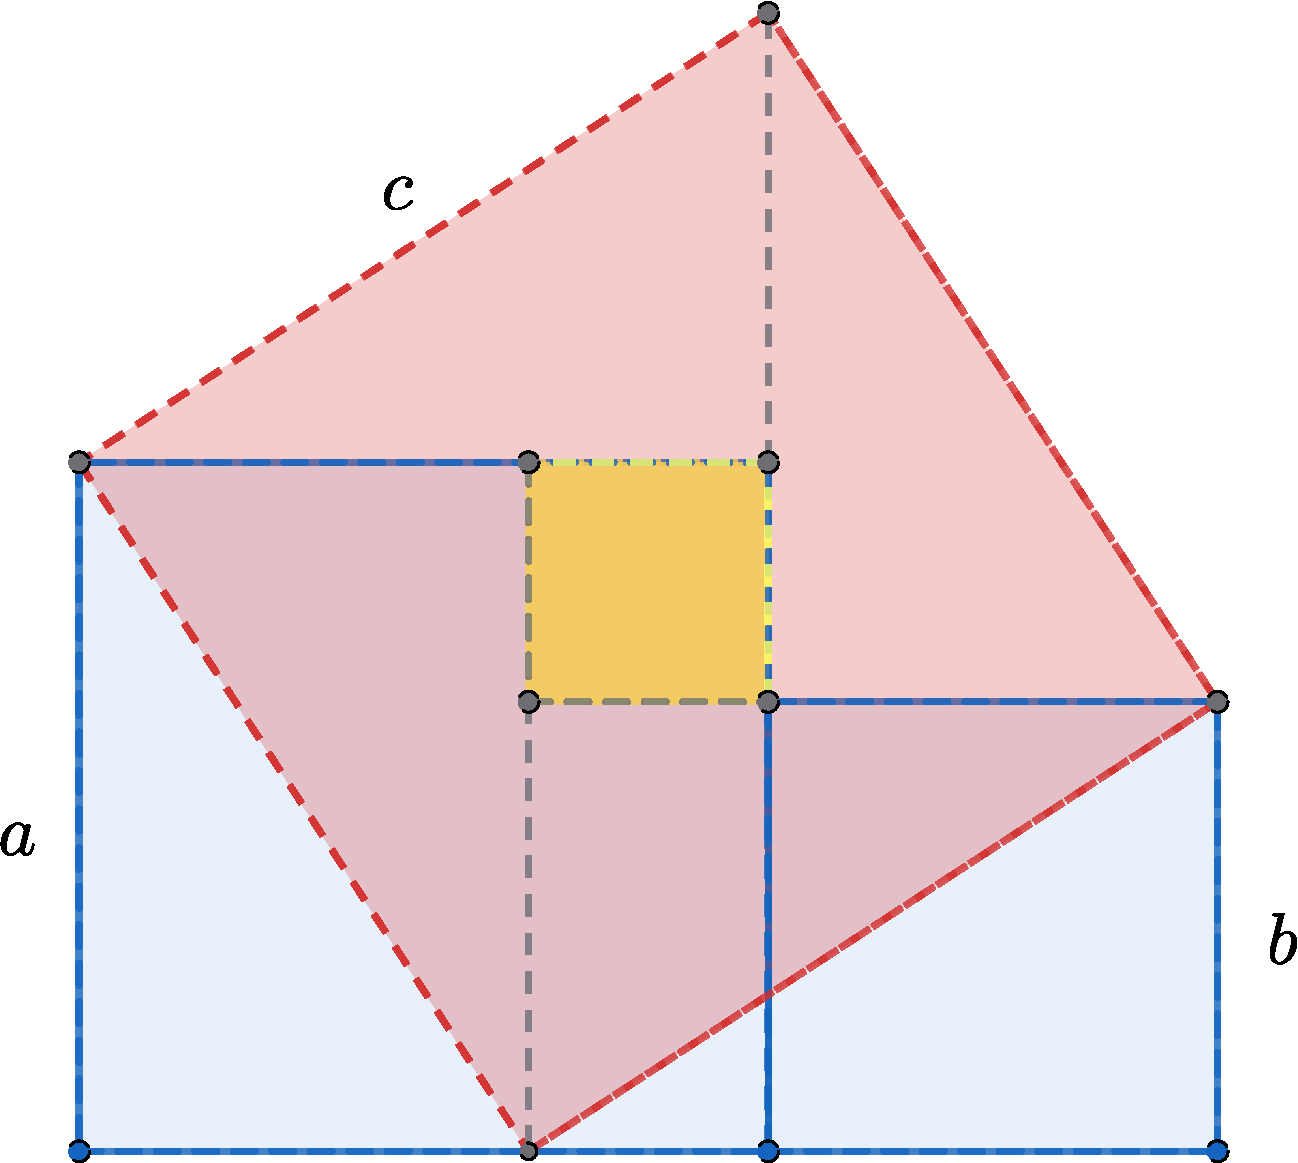
\includegraphics[scale=0.2]{img/zhaoshuang}}
 \caption{赵爽弦图成为了2002年在北京召开的国际数学家大会和中国数学会的会徽。\label{fig:cms-zhaoshuang}}
\end{figure}

这一定理自提出以来,吸引了无数聪明的头脑对它进行证明。如今在中学数学课堂上就至少有“赵爽弦图”(见\cref{fig:cms-zhaoshuang}),传说中的“毕达哥拉斯证法”(见\cref{fig:pythagoras-pww})和《原本》证法。在4000年的时间里,诞生了超过300多种不同的证明,包括意大利文艺复兴时期的全才达·芬奇(见\cref{fig:davinci})和美国总统加菲尔德。

\begin{figure}[htbp]
 \centering
 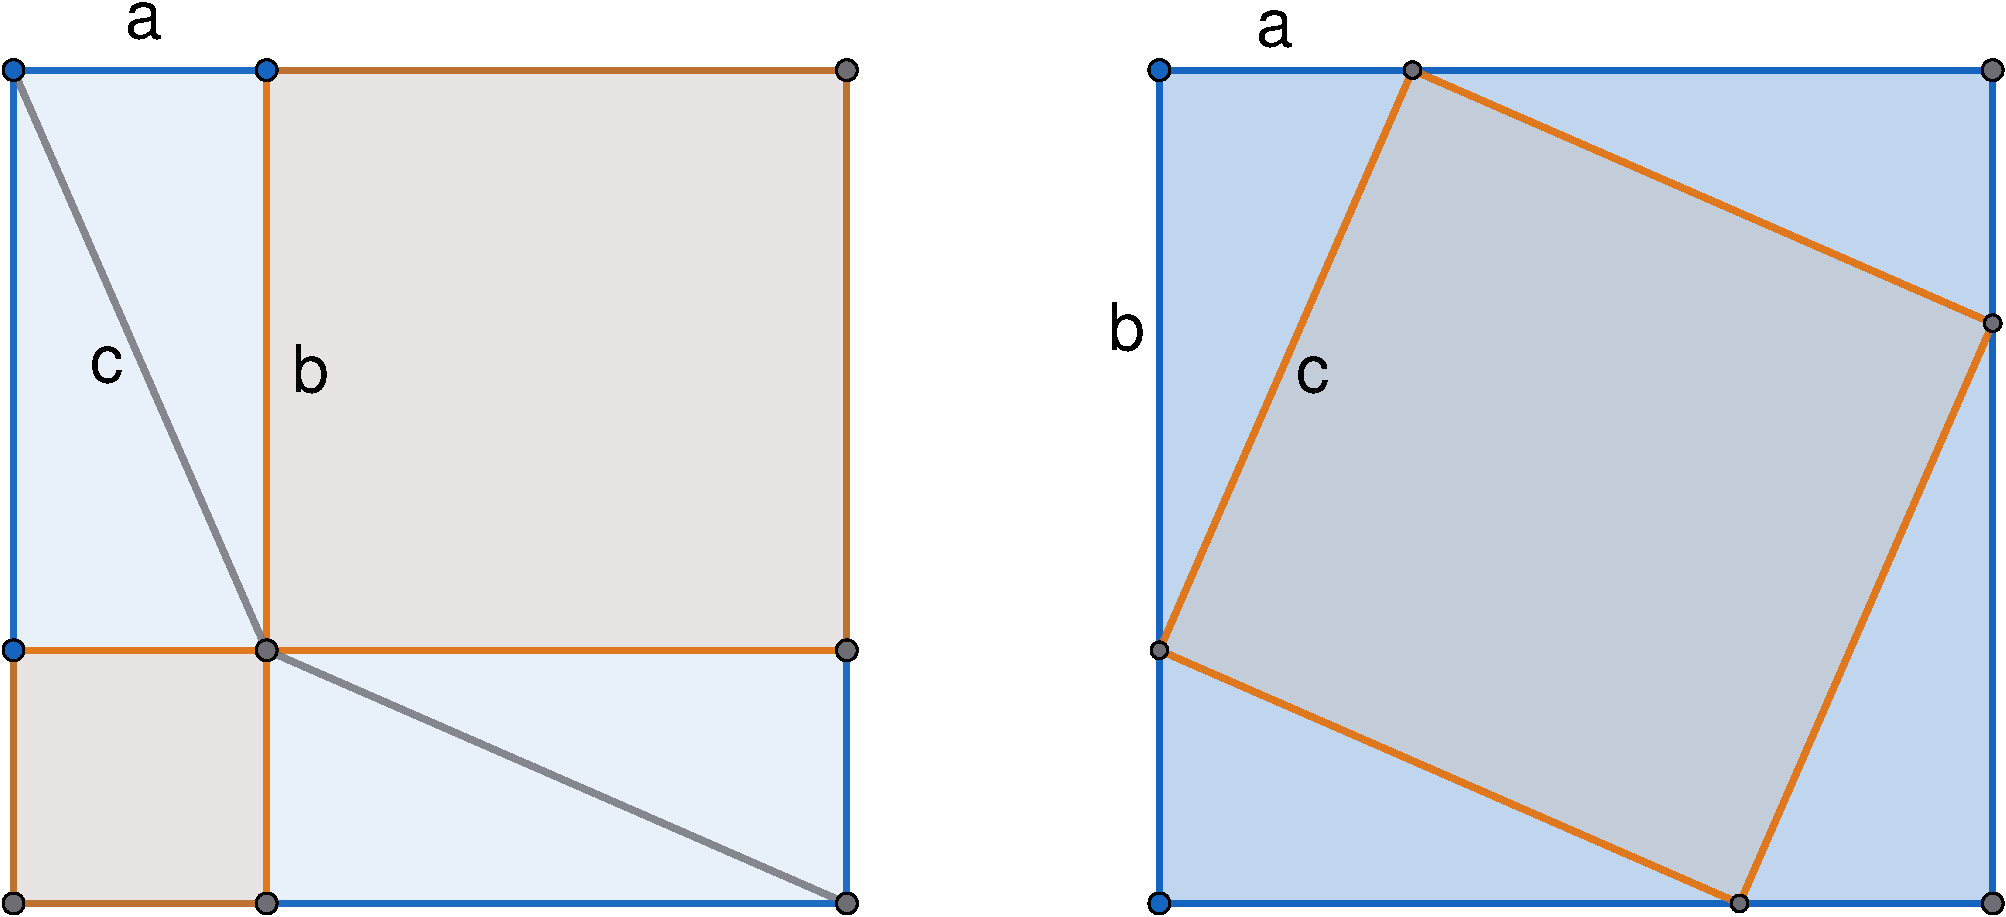
\includegraphics[scale=0.25]{img/pythagoras-pww}
 \caption{传说中的毕达哥拉斯证法\label{fig:pythagoras-pww}}
\end{figure}

达·芬奇的方法把原直角三角形复制两份:一份上下颠倒拼到上方,一份平移拼到斜边组成的正方形下方。此时把\cref{fig:davinci}中的“T”形点划线上方的四边形左右镜像翻转,就拼出一个和下方全等的六边形。它们的面积相等,因此各自减去两个原直角三角形的面积后仍相等,即$a^2 + b^2 = c^2$。\cref{qn:pythagoras-thm-garfield}要求解释美国总统加菲尔德的证明方法。

\begin{figure}[htbp]
 \centering
 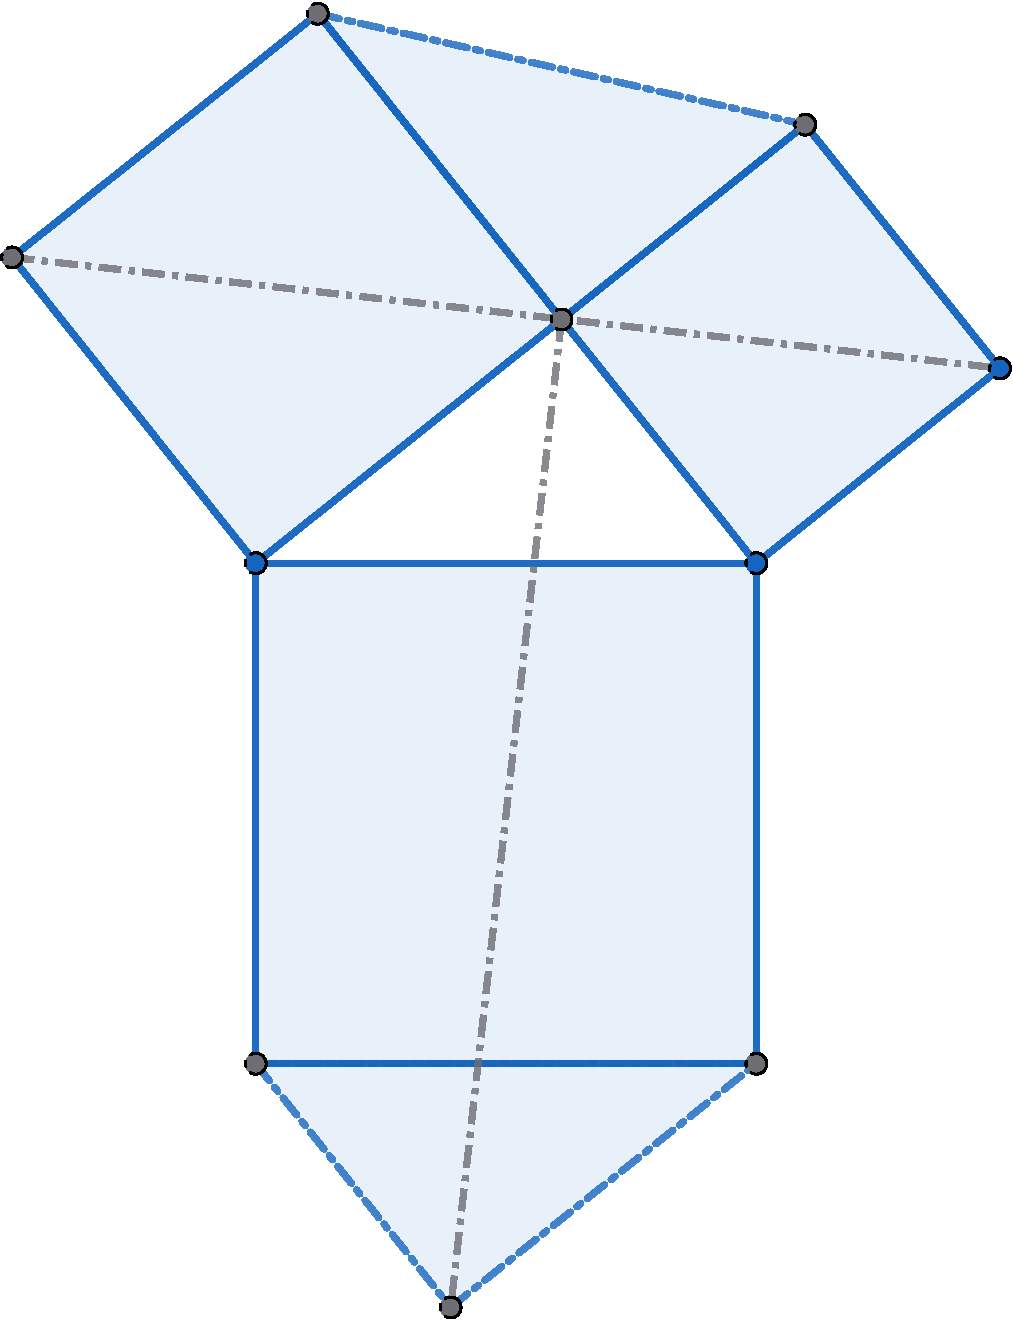
\includegraphics[scale=0.3]{img/davinci}
 \caption{列昂纳多·达·芬奇证法\label{fig:davinci}}
\end{figure}

勾股定理具有非凡的意义,犹如发源的清泉,流淌出了三条壮阔的大河\cite{Stillwell-2010}:1)数论,通过寻找哪些数构成勾股数(也叫做毕达哥拉斯三元组),古希腊人开启了数学皇冠上的明珠——数论的研究。2)几何,勾股定理本身就是一条定量的几何定理。3)无穷,把勾股定理和欧几里得算法结合,古希腊人被无穷次的递归困扰,直接导致了无理数的发现。

\section{数论}
并非任意两个平方数的和一定是平方数,例如$3^2 + 5^2 = 34$不是任何正整数的平方。我们把满足勾股定理的三个正整数$(a, b, c)$叫做勾股数或毕达哥拉斯三元组\footnote{Pythagoras triple}。各个文明都发现了常见的勾股数如$3^2 + 4^2 = 5^2$,$5^2 + 12^2 = 13^2$。古巴比伦的石板上刻有长长的勾股数表。那么究竟怎样找到勾股数?勾股数是有限多还是无限多?这个问题是欧几里得彻底解决的。欧几里得指出,如果$a^2 + b^2 = c^2$成立,那么这组勾股数的倍数也是勾股数,因为:

\begin{align*}
(ka)^2 + (kb)^2 &= k^2(a^2 + b^2) & \text{分配律} \\
  &= k^2c^2 & \text{由}a^2 + b^2 = c^2 \\
  &= (kc)^2
\end{align*}

反过来,如果$a, b$含有公因子$k \ne 1$,则$k$一定也是$c$的因子。同理,如果$b, c$含有公因子$k$,则由于$a^2 = c^2 - b^2$,所以$k$一定也是$a$的因子。本质上我们只需要寻找彼此互素的$a, b, c$(公因子只有1,或$(a, b) = (b, c) = 1$,见\ref{sec:gcd-minus}节),然后乘上倍数就得到更多的勾股数。例如勾股数(12, 16, 20)都是偶数,显然含有公因子2。分别除以2就得到更“简单”的勾股数(6, 8, 10)。继续除以2得到(3, 4, 5)。此时3、4、5彼此互素,已经不能再化简了。我们不妨称这样的勾股数为“最简勾股数”。由于$a$和$a^2$的奇偶相同:奇数的平方还是奇数,偶数的平方还是偶数。如果$a, b$一奇一偶,则$c$一定是奇数。欧几里得进一步排除了$a, b$都是奇数的情况,因为:

\begin{align*}
a^2 + b^2 &= (2m + 1)^2 + (2n + 1)^2 & \text{把}a, b\text{写成奇数形式} \\
  &= 4m^2 + 4m + 1 + 4n^2 + 4n + 1 & \text{分别用完全平方公式展开} \\
  &= 4(m^2 + m + n^2 + n) + 2 = 4k + 2 & \text{令整数} k = m^2 + m + n^2 + n
\end{align*}

这个值除以4余2。但是不管$c$是奇数还是偶数,$c^2$除以4都不可能余2。因为:偶数$(2k)^2 = 4k^2$被4整除,而奇数$(2k + 1)^2 = 4(k^2 + k) + 1$除以4余1。因此$a$和$b$不可能都是奇数,只能是一奇一偶。我们可以任选一个(比如第一个)为偶数,另一个是奇数。这样问题就化简为寻找第一个数为偶数,彼此互素的勾股数。它的答案赫然出现在《几何原本》卷十中的引理1\footnote{《几何原本》中使用正方形代表平方数,并用语言描述做法,见\citepage[330页]{Elements}。这里使用代数符号方便理解。}。

\begin{lemma}[欧几里得《几何原本》卷十,引理1]
方程$x^2 + y^2 = z^2$其中$x, y, z$彼此互素,且$x$是偶数的\underdot{所有}正整数解,可表示为:
\be
\begin{cases}
x = 2mn \\
y = m^2 - n^2 \\
z = m^2 + n^2
\end{cases}
\ee
其中$m > n$,是奇偶不同且互素的任意正整数。
\end{lemma}

注意“所有”二字,这意味着不存在其它最简勾股数能逃出欧几里得的解。换言之,这是\underdot{充分必要}条件。我们接下来证明这一优美的结论。

\begin{proof}
首先正向证明充分性:

\begin{align*}
x^2 + y^2 &= (2mn)^2 + (m^2 - n^2)^2 & \text{代入} \\
  &= 4m^2n^2 + m^4 + n^4 - 2m^2n^2 & \text{完全平方公式展开} \\
  &= m^4 + n^4 + 2m^2n^2 = (m^2 + n^2)^2 &\text{反向用完全平方公式} \\
  &= z^2 &\text{代入}z
\end{align*}

接下来反向证明必要性。把$x^2 + y^2 = z^2$移项后用平方差公式:
\begin{align}
x^2 &= z^2 - y^2 = (z + y)(z - y) &\text{平方差公式} \label{eq:x-as-z-pm-y} \\
(\frac{x}{2})^2 &= (\frac{z + y}{2}) (\frac{z - y}{2}) &\text{左右同除以4}
\end{align}

$x$是偶数,$y, z$都是奇数,故$z \pm y$都是偶数。因此左边的$\frac{x}{2}$,右边的$\frac{z \pm y}{2}$都是正整数。进一步,由于$z, y$互素,所以$\frac{z + y}{2}$和$\frac{z - y}{2}$也互素(见\cref{qn:coprime-of-half-a-pm-b})。如果两个互素的数的乘积是一个平方数,则它们也都是平方数(见\cref{qn:coprime-product-as-square})。因此:

\begin{align*}
\frac{z+y}{2} &= m^2 \\
\frac{z-y}{2} &= n^2
\end{align*}

其中正整数$m > n$。两式相加消去$y$求得$z = m^2 + n^2$,两式相减消去$z$求得$y = m^2 - n^2$。代入\cref{eq:x-as-z-pm-y}得:$x^2 = 2m^2 2n^2$,故$x = 2mn$。
\end{proof}

例如取$m = 2, n = 1$就得到(3, 4, 5),取$m = 3, n = 2$就得到(12, 5, 13)。而所有勾股数的就可以表示为:

\be
x = 2mnr, \quad y = r(m^2 - n^2), \quad z = r(m^2 + n^2)
\ee

其中$r$是任意正整数。

\begin{figure}[htbp]
 \centering
 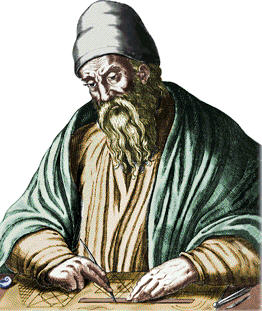
\includegraphics[scale=0.6]{img/Euclid}
 \caption{欧几里得,约公元前300年前后}
 \label{fig:Euclid}
\end{figure}

\begin{mdframed}

\index{欧几里得}
欧几里得(Euclid)是古希腊数学家,以其所著的《几何原本》闻名于世。对于他的生平,现在知道的很少。柏拉图学派晚期的导师普罗克洛斯(Proclus)在《几何学发展概要》中记述了这样的趣事:当时的埃及国王,亚历山大的托勒密一世有一次问欧几里得,学习几何学又没有什么捷径可走。欧几里得回答到:“在几何里,没有专为国王铺设的大道。\footnotemark”(There is no royal road to geometry),学习没有捷径成为了千古传颂的箴言。斯托比亚斯(Stobaeus)记述另一则故事说。一个学生刚开始学习第一个命题,就问欧几里得学习几何后将得到什么。欧几里得说:“给他三个钱币,因为他想在学习中获取实利。”由此可知欧几里得主张学习必须循序渐进、刻苦钻研、不赞成投机取巧的作风,也反对狭隘的实用观点\cite{Elements}。

欧几里得的《几何原本》是一部划时代的著作。其伟大的历史意义在于它是用公理建立起演绎体系的最早典范。过去所积累下来的数学知识是零碎的、片断的,可以比作木石砖瓦。只有借助于逻辑方法,把这些知识组织起来,加以分类比较,解释彼此间的内在联系,整理在一个严密的系统之中,才能建成巍峨的大厦。《几何原本》完成了这一艰巨的任务,它对整个数学的发展产生了深远的影响。

《几何原本》的英文译作The thirteen books of Euclid's elements,直译成中文是欧几里得原本十三卷,简称《原本》(英文简称Elements)。这十三卷包含几何、恒等式、比例论、数论、无理量、穷竭法、正多面体等内容,是古希腊数学的集大成者。明代末年,《原本》前六卷传入中国,学者徐光启和传教士利玛窦与1607年合作将其翻译成中文。可能是因为前六卷集中于几何学(第七到十卷才包含数论),徐光启将其命名为《几何原本》。其中译定的一些重要术语沿用至今。遗憾的是,利玛窦的去世和明清之际的剧变中断了后七卷的翻译工作。直到250年后的1857年,中国数学家李善兰和英国传教士伟烈亚力才将完整的《几何原本》译出。他们以英译本为底本,译出了后九卷,包括被认为是后人添加的第14,15卷。李善兰曾在曾国藩军中效力,他把译稿交给曾国藩说,松江刻本已经毁于战乱了,如果不再出版,这样的绝学就会失传(“此算学家不可少之书,失今不刻,行复绝矣。”)。曾国藩嘱托李善兰把前六卷重新订正,汇集在一起。同治四年(1865年)十月,曾国藩为此书作序,并主持重刻出版。这推动了《几何原本》在近代中国的传播和影响。考虑到这十三卷的内容不仅包含几何,今天在部编版中小学数学教材中,已经统一使用《原本》这个译法。我们也推荐读者朋友们使用《原本》或者《欧几里得原本》这样的叫法。
%% https://www.zhonghuashu.com/wiki/%E5%B9%BE%E4%BD%95%E5%8E%9F%E6%9C%AC/%E5%BA%8F

两千多年来,这部著作在几何教学中一直占据统治地位,在二十世纪初依然用于数学课的基本教材。包括我国在内的许多国家仍将其作为中学的必修科目(现在中学的几何课本是按照法国数学家勒让德《原本》改写本思路编写的),并作为训练逻辑推理的最有力教育手段\cite{HanXueTao16}。
\end{mdframed}
\footnotetext{也译为“几何无王者之道”}

尽管彻底解决了$x^2 + y^2 = z^2$的所有整数解问题,但$x^3 + y^3 = z^3$,$x^4 + y^4 = z^4$,或者更一般的$x^n + y^n = z^n$(其中整数$n \geq 3$)却难住了古人。似乎除了$x = y = z = 0$再也找不出任何整数解了。我们要等到1800年后的十七世纪,青年“业余”数学家费马才在$n = 4$上获得突破(见第6章)。勾股定理的整数解问题展示了数论这一数学分支的典型问题:研究数,特别是整数的性质。在很长一段时间,这门学科被称为“算术”(arithmetic),例如古希腊数学家丢番图的名著《丢番图算术》,德国数学家高斯的化时代著作《算术研究》都是数论方面的经典。奇偶性、素数、整除、公因子,余数等概念是这门学科的基础概念。在“长方形数”的探索中,古希腊人发现某些数可以表示成长方形,如$12 = 3 \times 4$可以用三行四列的小石子摆出。这样就引出了因数的概念,长方形数的边长就是其因子。并且因子可能有多个,例如$12 = 3 \times 4 = 2 \times 6$,所以2、3、4、6都是12的因子。但是有些数却无法表示成长方形数,例如5,只能摆成一行五个石子或一列五个石子\footnote{显然古希腊人在这里区分了线段和矩形,他们并不认可$1 \times 5$或$5 \times 1$是一个长方形数。}。这种数形结合的方法引出了素数的概念。素数$p$只能被1和$p$整除,是构成其它数的砖石。前几个素数是2、3、5、7、11……这样的探索自然引出了有趣的问题:1)作为构成其它数的砖石,素数有多少个?是有限多还是无限多?2)素数的出现有何规律?有没有产生素数的公式和方法?其中第一个问题又是由欧几里得解决的,而埃拉托斯特尼在第二个问题上迈出了关键的第一步。

自从芝诺悖论提出后,古希腊人就试图避免无穷这个概念。亚里士多德认为所有芝诺悖论中的问题都源自无穷,他提出了一个影响至今的区分:潜无穷和实无穷\footnote{英文分别是potential infinity和actual infinity}。所谓潜无穷或潜无限,是指无限在永远延伸着,是一种变化的、不断产生出来概念。它永远在构造中,永远完成不了,是潜在的,而不是实在的。自然数就是一种潜无穷,对于任何一个自然数$n$,我们都可以找到它的后继$n + 1$,也就是一个更大的自然数。欧几里得几何中的直线也是一种潜无穷,我们可以按需延伸直线。所谓实无穷是指把无限的整体本身作为一个实在的单位,是已经构造出来的东西。也就是把无限对象看作可完成的过程或无穷整体。在做了这种区分后,亚里士多德承认存在潜无穷,但是拒绝承认实无穷的概念。他对实无穷的排斥深刻而长远地影响了日后数学的发展\cite{HanXueTao16}。亚里士多德代表了当时古希腊的哲学观点,关于潜无穷和实无穷的概念区分以及争论一直影响至今。纵观《原本》全书,欧几里得从未在其中使用“无穷”或者“无限”一词。尽管如此他还是成功证明了素数有无限多个,并且这一证明被人们认为是历史上最优美的证明证明之一。

\begin{theorem}[欧几里得《原本》第九卷,命题20]
预先给定任意多的素数,则有比它们更多的素数。
\end{theorem}

欧几里得在叙述这个命题时,小心谨慎地避免使用无穷这样的说法。“预先给定……总有更多的……”这种处理经常出现在《原本》中。我们今天往往直接说“存在无穷多的素数”。欧几里得在证明这个命题时,使用了著名的反证法。我们用现代的语言来描述这一证明。

\begin{proof}
假设只存在有限多个素数,$p_1, p_2, \dotsc, p_n$。欧几里得构造一个新数:
\[
p_1 p_2 \dotsm p_n + 1
\]
也就是把这$n$个素数乘起来再加一。这个数要么是素数,要么不是素数。

\begin{itemize}
\item 如果它是素数,明显这个数不等于$p_1$到$p_n$中的任何一个,这就在有限多个素数之外又增加了一个新的素数;
\item 如果这个数不是素数,那么它就存在一个素因子$p$。但是由于$p_1$到$p_n$中的任何一个都不能整除构造的这个数(除不尽余1),所以素数$p$与任何$p_1$到$p_n$中的数都不同,是一个新的素数。
\end{itemize}
所以在任何情况下,我们都可以获得一个新的素数。这与有限个素数的假设矛盾,因此存在无穷多的素数。
\end{proof}

欧几里得用反正法得到了一种“存在性证明”,他证明了存在无穷多的素数,但却没有给出怎样得到这些素数。这在我们今天看来,是很自然的一种处理。然而在十九世纪末二十世纪初却引发了关于数学根本性的争论。迄今为止,人们没有发现任何素数公式。我们不说“计算”出素数”,而只能说寻找素数。一个非常低效的方法是从$2, 3, 4, \dotsc$开始逐一检查每个数$n$是否是素数。根据定义,需要检查$n$是否含有1和$n$之外的其它因子。这需要依次判断$2, 3, \dotsc, n - 1 $是否整除$n$。当然,由于$a \times b = b \times a$,我们可以把这个范围缩小到判断$2, 3, \dotsc, \lfloor \sqrt{n} \rfloor$是否整除$n$,即把上限定为不大于$n$的开平方的整数。这个方法很差,除法的计算量非常大。埃拉托斯特尼给出了一种快速寻找素数的方法,被称为埃拉托斯特尼筛法。首先我们列出从2开始的整数:

\[2, 3, 4, 5, 6, 7, 8, 9, 10, 11, 12, 13, 14, 15, 16, 17, 18, 19, 20, \dotsc \]

2是第一素数。然后从2开始,筛除掉所有2的倍数:

\[2, 3, \cancel{4}, 5, \cancel{6}, 7, \cancel{8}, 9, \cancel{10}, 11, \cancel{12}, 13, \cancel{14}, 15, \cancel{16}, 17, \cancel{18}, 19, \cancel{20}, \dotsc\]


接下来的3就是第一轮筛除后新找到的素数。然后再筛除3的倍数:

\[2, 3, 5, 7, \cancel{9}, 11, 13, \cancel{15}, 17, 19, \cancel{21}, 23, 25, \cancel{27}, 29, \dotsc\]

接下来的5是新找到的素数。然后筛除掉所有5的倍数:

\[2, 3, 5, 7, 11, 13, 17, 19, 23, \cancel{25}, 29, \dotsc\]

每轮筛除后,剩余的第一个数$p$是新找到的素数,接下来的一轮筛除掉所有$p$的倍数。这样不断进行下去。通常在应用埃拉托斯特尼筛法时,我们事先定出一个目标:寻找$n$以内的素数。接下来不断进行筛除,直到把不大于$\sqrt{n}$的所有倍数都筛除为止。\cref{qn:seive-of-eratosthenes-100}要求利用筛法找出100以内的所有素数。

有了因子的概念,毕达哥拉斯学派开始研究这些因子和数的关系。他们发现某些数的所有真因子\footnote{真因子是小于数本身的因子}之和恰好等于这个数本身,于是将其命名为完美数(也叫做完全数),并成功地找到两个。最小的完美数是6,因为6的真因子有1、2、3,而6 = 1 + 2 + 3,下一个是28,其真因子为1、2、4、7、14,并且28 = 1 + 2 + 4 + 7 + 14。毕达哥拉斯学派并非纯粹的学术团体,学派信奉数字神秘主义。他们对完美数如此着迷,认为:“6象征着完满的婚姻以及健康和美丽,因为它的部分是完整的,并且其和等于自身。”中世纪后,更是赋予了完美数宗教意义。人们认为6和28是上帝创造世界时所用的基本数字,因为上帝创造世界花了六天,二十八天则是月亮绕地球一周的日数。真正从数论的角度对完美数进行研究并取得关键进展的还是欧几里得。

\begin{theorem}[欧几里得《原本》卷九,命题36]
如果$2^{n+1}-1$是素数,则$2^n(2^{n+1}-1)$是完美数\footnote{这里用代数符号简化了叙述,《原本》原文为:设从单位起有一些连续二倍起来的连比例数,若所有数之和是素数,则这个和乘最后一个数的乘积将是一个完全数。进行对比,不难看出代数符号的威力。}。
\end{theorem}

\begin{proof}
素数$p = 2^{n+1}-1$只有两个因子$1, p$;$2p$含有四个因子$1, 2, p, 2p$;$4p = 2^2p$含有6个因子$1, 2, 4, p, 2p, 4p$;以此类推$2^n p$含有$2(n+1)$个因子$1, 2, 4, \dotsc, 2^n, p, 2p, 4p, \dotsc, 2^n p$。最后一个不是真因子,剩余的真因子和为:

\begin{align*}
s &= 1 + 2 + \dotsb + 2^n + p + 2p + \dotsb + 2^{n-1}p \\
  &= (1 + 2 + \dotsb + 2^n) + p(1 + 2 + \dotsb + 2^{n-1})
\end{align*}

我们在高中学习过等比数列求和,这里不妨用方程从头推导一下。令:

\be
x = 1 + 2 + 4 + \dotsb + 2^n
\label{eq:sum-of-power2}
\ee

把\cref{eq:sum-of-power2}乘以2:

\be
2x = 2 + 4 + 8 + \dotsb + 2^n + 2^{n+1}
\label{eq:2sum-of-power2}
\ee

\cref{eq:2sum-of-power2}减\cref{eq:sum-of-power2}得:

\begin{align*}
2x - x & = \quad \ \cancel{2} + \cancel{4} + \dotsb + \cancel{2^n} + 2^{n+1} \\
       & - 1 - \cancel{2} - \cancel{4} - \dotsb - \cancel{2^n} \\
  x &= 2^{n+1} - 1
\end{align*}

把这个结果代入真因子和求$s$:

\begin{align*}
s & = 2^{n + 1} - 1 + p(2^n - 1) &&\text{代入}p = 2^{n+1} - 1 \\
  & = p + 2^n p - p = 2^n p = 2^n (2^{n+1} - 1) && \qedhere
\end{align*}
\end{proof}

所以$2^n(2^{n+1}-1)$是完美数。后人把这一形式的完美数称为欧几里得完美数。根据欧几里得的结果,不难看出:1)只要找到更多的形如$2^{n+1} - 1$的素数,就能找到更多的完美数。2)所有欧几里得完美数都是偶数,但完美数一定是偶数吗?很容易验证毕达哥拉斯学派的找到的6和28都是欧几里得完美数:$2^1\times(2^2-1)=2 \times 3 = 6$,$2^2 \times (2^3 - 1) = 4 \times 7 = 28$,分别是$n = 1, n = 2$时的情况。但后面就没有这么幸运了。$2^4 - 1 = 15$不是素数。不过$2^5 - 1 = 31$是素数,所以$2^4 \times 31 = 16 \times 31 = 496$是下一个完美数。但$2^6 - 1 = 63$不是素数,$2^7 - 1 = 127$是素数,所以$2^6 \times 127 = 8128$是完美数。接下来$n = 8, 9, 10, 11, 12$都不是素数,下一个素数是$2^{13}-1 = 8191$。凭借手算验证这个数是素数已经很困难了,其对应的完美数更是巨大到了33550336。欧几里得完美数的增加极其快速,由于古希腊人没有强大的位值制十进制计数系统,寻找更多完美数的研究遇到了困境。而问题2)的难度远非常人想象。数学家欧拉进一步证明了,任何偶完美数必然是欧几里得完美数(见附录\ref{app:even-perfect-number})。古希腊人没有找到任何奇完美数。不仅如此,直到今天也没有发现任何奇完美数。于是人们猜想不存在奇完全数,但迄今为止没有人能证明这个猜想。这成了当今数学中的悬案,吸引了从欧拉到陶哲轩一代又一代数学家对它进行研究。

十七世纪,法国神父梅森和数学家费马通过书信往来继续研究了形如$2^n \pm 1$的素数。费马于1640年给出了一个惊人的“素数公式”:

\be
F_n = 2^{2^n} + 1
\ee

计算不难发现:$F_0 = 2^{2^0} + 1 = 3$是素数,$F_1 = 2^{2^1} + 1 = 5$是素数,$F_2 = 2^{2^2} + 1 = 17$是素数,$F_3 = 2^{2^3} + 1 = 257$是素数,$F_4 = 2^{2^4} + 1 = 65537$还是素数。费马高兴地断言,所有$F_n = 2^{2^n} + 1$都是素数!我们可以想像手工验算65537的难度,并且这个指数的指数“爆炸”速度极为惊人。费马的猜测令人兴奋,因为从未有人发现任何有效的产生素数的公式。今天我们称$F_n$为费马数。但是近一个世纪后,大数学家欧拉于1732年发现:$F_5= 641 \times 6700417$是一个合数。并且从那以后,人们利用手算或计算机验算了$F_5$到$F_{30}$,很不幸它们都是合数。是否$n = 5$以后所有的$F_n$都是合数至今仍然是一个未证明的猜想。故事并未结束,第X节我们将会看到费马数惊人地出现在正多边形尺规作图的背后。

\begin{mdframed}
你也许好奇,欧拉是如何手算找到$F_5$的因子的。这是多么巨大的计算量啊!但欧拉就是欧拉,他可能是通过这一巧妙的方法完成对$F_5$的因子分解的\citepage[27页]{Coxeter2022}\citepage[18页]{Hardy2009}。欧拉重新发现费马的研究成果后,必定对费马大定理$x^n + y^n = z^n$感兴趣。在研究四次方和($n = 4$)时很容易遇到$5^4 + 2^4= 641$。而费马数$F_5 = 2^{2^5} + 1 = 2^{32} + 1$。注意到把$641 = 5^4 + 2^4$乘以$2^{28}$就能凑到$2^{32}$:
\[
641 \times 2^{28} = (5^4 + 2^4)2^{28} = 5^42^{28} + 2^{32} = A
\]

令这个数为$A$。从$A$中减去$5^42^{28}$再加上1就是费马数$F_5$,令$B = 5^42^{28} - 1$,则$F_5 = A - B$。另一方面$641 = 640 + 1 = 5 \times 128 + 1 = 5 \times 2^{7} + 1$。注意到它是$B$的一个因子!我们可以两次用平方差公式对$B$进行因式分解:

\begin{align*}
B = 5^4 2^{28} - 1 &= (5^2 2^{14} + 1)(5^2 2^{14} - 1) && \text{平方差公式} \\
  &= (5^2 2^{14} + 1)(5 \times 2^7 + 1)(5 \times 2^7 - 1) && \text{对第2项用平方差公式} \\
  &= (5^2 2^{14} + 1) \times 641 \times (5 \times 2^7 - 1)
\end{align*}

由于641既整除$A$也整除$B$,所以641整除$A - B = F_5$。这样就证明了费马数$F_5$不是素数。这一年(1732年),欧拉只有25岁。
\end{mdframed}

与费马通信、讨论后,梅森对形如$2^n - 1$的素数进行了大量的计算、验证,并取得了重要的进展。我们不知道如下的结论是来自费马、梅森,还是来自后人:

\begin{proposition}[梅森素数]
如果$n > 1$且$a^n - 1$是素数,则必然有$a = 2$并且$n$是素数。
\end{proposition}

\begin{proof}
可以利用等比数列求和公式证明$a = 2$。考虑下面的等比数列:

\begin{align*}
s  &= 1 + a + a^2 + \dotsb + a^{n-1}  \\
as &= a + a^2 + \dotsb + a^{n-1} + a^n && \text{两边乘以}a \\
as - s &= \cancel{a} + \cancel{a^2} + \dotsb + \cancel{a^{n-1}} + a^n - 1 - \cancel{a} - \cancel{a^2} - \dotsb - \cancel{a^{n-1}} \\
(a - 1)s &= a^n - 1 \\
 s &= \frac{a^n - 1}{a - 1}
\end{align*}

这说明$a - 1$是$a^n - 1$的一个因子\footnote{也可以用函数的方法证明这点:考虑函数$f(x) = x^n - 1$,显然$x = 1$是方程$f(x) = 0$的一个解:$1^n - 1 = 0$。因此$x-1$是$x^n - 1$的因子。},但如果$a^n - 1$是素数,它只有1和自己两个因子。这样必然有$a - 1 = 1$,即:$a = 2$。

我们接下来证明$n$必然是素数。用反证法,假设$2^n - 1$是素数,但$n = ab$不是素数,可以分解为两个大于1的数的积。考虑等比数列的和:
\[
s = 1 + 2^a + (2^a)^2 + (2^a)^3 + \dotsb + (2^a)^{b-1}
\]

其中每项都是前一项的$2^a$倍。两边同时乘以$2^a$再减去原数列,消去除首尾的中间项得:

\[
s = \frac{(2^a)^b - 1}{2^a - 1} = \frac{2^{ab} - 1}{2^a - 1}
\]

这说明$2^a - 1$整除$2^{ab} - 1$。并且根据假设$a > 1$,有$2^a - 1 > 1$。这与$2^n - 1 = 2^{ab} - 1$是素数矛盾。所以$n$必然是素数。
\end{proof}

注意,这一命题的逆命题\underdot{不成立}。$p$是素数时,$2^p - 1$不一定是素数。例如$2^{11} - 1 = 2047 = 23 \times 89$。但这一命题使得梅森只需要寻找形如$2^p - 1$的素数。1644年,梅森在他的著作《物理数学随感》\footnote{拉丁文Cogitata Physica-Mathematica}的前言中断言:在$257$以内,只有$p$等于2, 3, 5, 7, 13, 17, 19, 31, 67, 127, 257时$2^p - 1$才是素数。尽管这一列表有两处错误(有两个不是素数,但缺失了两个真正的素数,正确的列表应为:2, 3, 5, 7, 13, 17, 19, 31, 61, 89, 107, 127)梅森的发现仍然极为重要。今天,人们定义这样的素数为梅森素数,记为$M_p = 2^p - 1$。尽管没有费马数那样“指数的指数级爆炸”,梅森素数依然是“指数爆炸”式增长的,没有人能轻易验证$M_p$是否是素数。直到1750年,欧拉才验证了$M_{31}$的确是素数。但即使是欧拉也错误地断言$M_{41}$和$M_{47}$是素数。人们直到1886年才发现梅森漏掉了$M_{61}$这个素数。1876年,法国数学家卢卡斯发现了一种检验梅森素数的方法,并成功确认了$M_{127}$是素数。这一素数长达39位。同时卢卡斯判定$M_{67}$不是素数,但是他并未找到其因子。1903年数学家科尔在一次数学会议上走上讲台,一言不发在黑板上写下:$2^{67} - 1 = 193707721 \times 761838257287$。面对台下的掌声,科尔说这花掉了了他三年来的每个星期天。今天人们利用计算机和互联网的强大算力寻找更多的梅森素数。截至2024年,人们共发现了52个梅森素数。其中第52个为$2^{136279841} - 1$共有41024320位。这个记录还在不断被打破。

\begin{figure}[htbp]
 \centering
 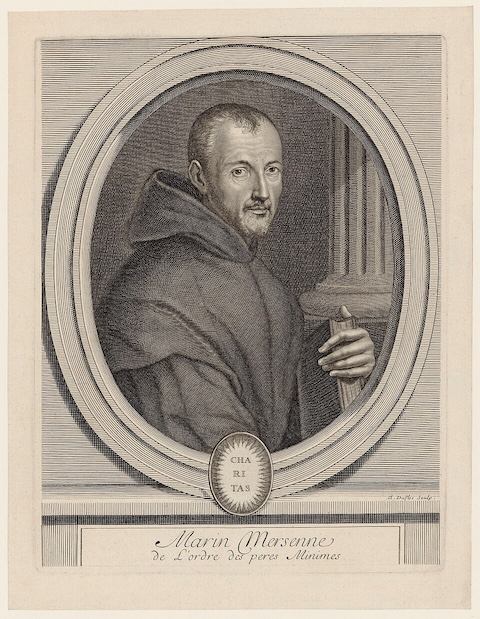
\includegraphics[scale=0.35]{img/MarinMersenne}
 %% https://commons.wikimedia.org/wiki/File:MarinMersenneDuflos.jpg
 \caption{克劳德·迪弗洛创作的版画:马林·梅森像}
 \label{fig:marin-mersenne}
\end{figure}

\begin{mdframed}
马林·梅森(Marin Mersenne, 1588~1648,见\cref{fig:marin-mersenne})是法国著名的修道士、自然哲学家、数学家。他是17世纪欧洲科学界中独特的中心人物。梅森与当时欧洲最伟大的思想家、科学家、数学家保持通信,定期组织学术讨论,发表并传播他们的成果,鼓励年轻的学者参与科学研究,极大地促进了法国和欧洲的科学和思想进步。

%% https://mathshistory.st-andrews.ac.uk/Biographies/Mersenne/
1588年9月8日,梅森生于法国一个普通工人家庭。尽管家庭经济条件不好,父母坚持让他接受教育。16岁时,梅森进入了拉弗莱什新成立的耶稣会学校。这所优秀的学校也招收穷人的子女,从这里走出了梅森和笛卡尔这些优秀的毕业生。1609年他从巴黎的索邦神学院毕业,并于1612年起担任神父。如果我们结合当时的历史背景,就会惊异于梅森如何成为了欧洲先进学术思想的中心人物。这是一件极为困难并且具有生命危险的工作。罗马教廷正在疯狂镇压新思想。哥白尼的《天体运行论》遭到封禁,布鲁诺遭遇火刑,伽利略被迫“认罪”,笛卡尔远走荷兰,帕斯卡假借外省人和索邦的神学家论战\footnotemark。作为神父的梅森却既得到教会的支持,又成为了各国科学家的秘密战友。我们不难想象他超人的沟通能力和受人尊敬的人格。

梅森热爱数学,他认为没有数学就没有科学。从1623年起,梅森小心翼翼地邀请欧洲的顶级学者到他位于巴黎的修道院访问,或者进行通信。有些人甚至远达君士坦丁堡和今天的罗马尼亚。梅森的常客包括佩雷斯克、伽森狄、笛卡尔、罗贝瓦尔、贝克曼、范·海尔蒙特、费马、霍布斯和帕斯卡父子。他每周组织会议,宣读或评议论文,交换学者间的联系方式,讨论实验或研究计划。这个以梅森为中心的小圈子俨然是今天的学术团体,被称为“巴黎学院”。由于梅森是中心人物,也被戏称为“梅森学院”。法国学术界认为,这是后来的法兰西科学院的前身。梅森的学者朋友越来越多,每当收到邀请,他就赶赴他国进行访问。

梅森喜爱音乐,他研究了声学理论和声音传播的速度。1627年他发表了《宇宙的和谐》一书,首次指出弦振动的频率正比于张力的平方根;反比于弦长、直径;反比于弦质量的平方根。梅森善于发现有才华的年轻人,鼓励他们分享想法和成果。年轻的罗贝瓦尔在巴黎的讨论会中崭露头角,梅森很快注意到了他,并建议他研究摆线这一课题。1638年,罗贝瓦尔成功计算出了摆线下的面积。年轻的惠更斯视梅森为榜样。在梅森的鼓舞下,他发表了《音乐的理论》一书。1644年10月,梅森访问了意大利,他了解到了伽利略的学生托里拆利进行的大气压实验(这一实验成功证实了大气是有重量的,大气压可以顶起约76厘米汞柱)。返回巴黎后,他组织学者们进行讨论,帕斯卡进一步通过实验验证了大气压随海拔的变化。可惜梅森没能看到实验结果就病逝了。今天,我们用帕斯卡作为国际压强单位以纪念这一研究。梅森几乎把他的一生献给了科学。1648年9月1日,梅森病逝于巴黎,他要求把自己的遗体用于生物学研究\cite{OConnor-Robertson-2005}。

%% https://www.britannica.com/biography/Marin-Mersenne
梅森的一些工作意义重大却极有风险。他帮助隐居于荷兰的笛卡尔出版了《谈谈方法》一书(被教会列为禁书),收集了主要学者对于笛卡尔《第一哲学沉思集》的反驳意见。在教会封禁的情况下坚持在法国出版了伽利略的著作,促进了新学术思想在欧洲的传播\cite{Britannia-2024}。梅森死后,人们从他的住所整理出了78位学者间的通信,包括费马、惠更斯、佩尔、伽利略、托里拆利等人,若干科学仪器以及大量书籍。这些文献后来被集结出版,成为了17世纪科学研究的宝贵财富。
\end{mdframed}
\footnotetext{见帕斯卡《致外省人信札》}

\section{无理数}
勾股定理(毕达哥拉斯定理)是一把双刃剑。一方面,它在几何、数论、分析等方向上产生了丰富的成果,另一方面它反过来攻击了毕达哥拉斯学派“万物皆数”的信念。与我们今天的概念不同,毕达哥拉斯学派的“数”指整数或者整数的比。所谓万物皆数是相信世间万物都可以表示为这样的数。如果自然界中存在某个量,但却不能表示成整数的比,那么毕达哥拉斯学派的根基就崩塌了。而勾股定理就是寻找这样的数的钥匙。由于这样的数不容于学派的哲学理念,所以被称为“无理数”,而整数或整数的比被称为“有理数”。整数与分数都是有理数,记为$\mathbb{Q}$,对应的英文是Quotient(商)。读者朋友们也许会问:有理数的英文是Rational numbers,为什么不用$\mathbb{R}$来表示有理数呢?这是因为字母$\mathbb{R}$被用来表示实数(英文Real numbers,见XX节),为了加以区分,数学家最终选用了$\mathbb{Q}$作为有理数的符号。它也的确更好地反映了有理数的本质属性(分数可表示为商,整数可表示成除数为1的商)。

古希腊\underdot{传说}希帕索斯(Hippasus)发现了无理数。这则故事为人们津津乐道,被说得有模有样。约公元前470年左右,毕达哥拉斯学派的学生希帕索思试图寻找正方形的对角线所代表的数。可是根据毕达哥拉斯定理,希帕索斯无论如何也找不到一个整数比能够等于正方形的对角线。他把这个发现告知学派的其他人,这造成了极大的恐慌。学派认为这将动摇他们在学术界的统治地位,于是极力封锁该真理的流传。希伯索斯被迫流亡他乡。不幸的是,他最终被毕达哥拉斯学派的门徒困在一条船上,并被沉入大海灭口。这则传说还有另外一个版本。毕达哥拉斯学派用五角星作为徽章和联络标志。希帕索思从神秘五角星标志上得到了启发。如果在边长为1的正五边形内画一个五角星,他发现五角星的对角线长度无法表示成整数的比,从而发现了无理数。这则传说反映了毕达哥拉斯学派的另一面:这个数字神秘主义团体更像是一个“兄弟会”。还有一则故事说,学派的一个成员流落异乡,贫病交迫,无力酬谢房主的款待,临终前要房主在门上画一个五角星。若干年后,有同派的人看到这个标志,询问事情的经过,厚报房主而去\cite{HanXueTao16}。美国迪士尼在1959年的动画片《唐老鸭漫游数学奇境》中,描绘了唐老鸭遇到了毕达哥拉斯和他的朋友们,在了解音乐、艺术与数的关系后,唐老鸭的手掌上也画上了神秘的五角星。

\begin{figure}[htbp]
 \centering
 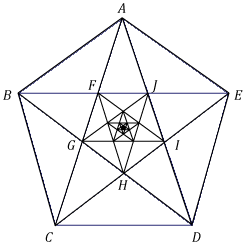
\includegraphics[scale=0.5]{img/pentagram}
 \caption{递归的五角星}
 \label{fig:pentagram}
\end{figure}

可是希帕索斯的传说经不起推敲,没有任何古代文献记录了这一事件。唯一与希帕索斯相关的说法来自亚里士多德,说希帕索斯与赫拉克利特都认为火是宇宙中的第一元素。毕达哥拉斯学派用五角星作为学派徽章,人们在用尺规绘制这一徽章的时候,能够轻易发现正五边形与正五角星相互嵌套以至无穷的特点(见\cref{fig:pentagram})。这些追寻宇宙奥秘的学者们不可能对此感到害怕和恐慌,而是感到好奇和着迷。说希帕索斯发现$\sqrt{2}$也很可疑,等腰直角三角形如此特殊,任何了解勾股定理的人都会发现这个特殊的值。根据亚里士多德的说法,毕达哥拉斯学派用归谬法(即反证法)证明了$\sqrt{2}$的无理性:

\begin{theorem}[毕达哥拉斯]
$\sqrt{2}$不能表示为整数的比,它是无理数。
\end{theorem}

\begin{figure}[htbp]
  \centering
  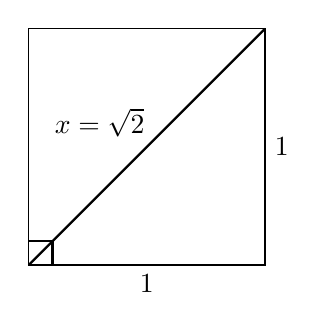
\begin{tikzpicture}[scale=3]
    \draw (0,0) -- (1,0) -- (1,1) -- (0,1) -- cycle;
    \draw[thick] (0,0) -- (1,1);
    \node[below] at (0.5,0) {$1$};
    \node[right] at (1,0.5) {$1$};
    \node[above, sloped] at (0.3,0.5) {$x = \sqrt{2}$};
    \draw[thick] (0.1,0) -- (0.1,0.1) -- (0,0.1);
  \end{tikzpicture}
  \caption{边长为1的正方形和对角线}
  \label{fig:square-diagonal}
\end{figure}

这一定理曾经以命题117出现在欧几里得《原本》卷十中。对比古代的版本,人们发现它是后人加入的。最新的《原本》已经删除了此定理。考虑边长为1的正方形和对角线(间\cref{fig:square-diagonal})。令对角线长为$x$,根据勾股定理有:$x^2 = 1^2 + 1^2 = 2$。记$x = \sqrt{2}$。我们这里给出两种证明方法,其中第一个证明来自毕达哥拉斯。

\begin{proof}
用反证法,假设$x$可以表示为即约分数$\frac{a}{b}$,其中$a, b$互素,且$b \ne 1$。我们有:
\begin{align*}
2 &= x^2 = (\frac{a}{b})^2  && \text{勾股定理} \\
a^2 &= 2b^2  && \text{两边乘以}b^2
\end{align*}
这说明$a^2$是偶数,所以$a$是偶数。令$a = 2c$,代入后得:
\begin{align*}
(2c)^2 &= 2b^2 \\
2c^2 &= b^2 && \text{两边除以}2
\end{align*}
这说明$b^2$也是偶数,因此$b$也是偶数。这与$a, b$互素矛盾。所以$x = \sqrt{2}$无法表示成即约分数,是无理数。
\end{proof}

第二个证明更加一般,它是寻找更多无理数的钥匙:
\begin{proof}
根据$a^2 = 2b^2$,并且$a, b$互素,一定有$b$整除$a^2$。因此$b$的任何素因子$p$也整除$a^2$。因为$p$是素数,所以$p$也整除$a$。这样$p$就既整除$a$也整除$b$,这与$a, b$互素矛盾。
\end{proof}

仔细观察这两个证明就会发现,毕达哥拉斯的证明实际是第二个证明的特殊情况:$p = 2$。下面我们就证明一个更强的定理:

\begin{theorem}
如果$n$不是某个整数的$m$次方,则$\sqrt[m]{n}$是无理数。
\end{theorem}

\begin{proof}
用反证法,假设$\sqrt[m]{n} = \frac{a}{b}$可以表示为即约分数,其中$a, b$互素,且$b \ne 1$。两边乘$m$次方得:
\[
a^m = n b^m
\]
这说明$b$整除$a^m$。因此$b$的任何素因子$p$一定也整除$a^m$。因为$p$是素数,所以$p$也整除$a$。这样$p$就既整除$a$也整除$b$,这与$a, b$互素矛盾。
\end{proof}

作为这个定理的特殊情况,如果$n$不是完全平方数,那么$\sqrt{n}$必然是无理数。这样古希腊人就通过几何量发现了无理数。谈到古希腊几何就一定会谈到尺规作图。顾名思义,就是只用直尺和圆规作图。按照古希腊哲学家柏拉图立下的传统,直尺是没有刻度的。所以其对应的英文是straight edge而非ruler。圆规一旦从平面上抬起,两脚就在重力的作用下自然合拢。这和我们今天使用的文具圆规有所不同。据说这样简陋的绘图工具源自古埃及的拉绳测量。把两点间的绳子绷直相当于画线段,后来演变成了直尺。把绳子的一段固定于某点,取定长的另一端自由移动相当于画圆,后来演变成了圆规。这看来简陋的绘图工具,在严格的规则限制下,却挑战着古希腊学者们的智慧,结出了欧几里得几何学的硕果。文艺复兴时代的伟大艺术家拉斐尔在他的旷世杰作《雅典学院》中描绘了专注用圆规作图的欧几里得(见\cref{fig:euclid-soa})。

\begin{figure}[htbp]
 \centering
 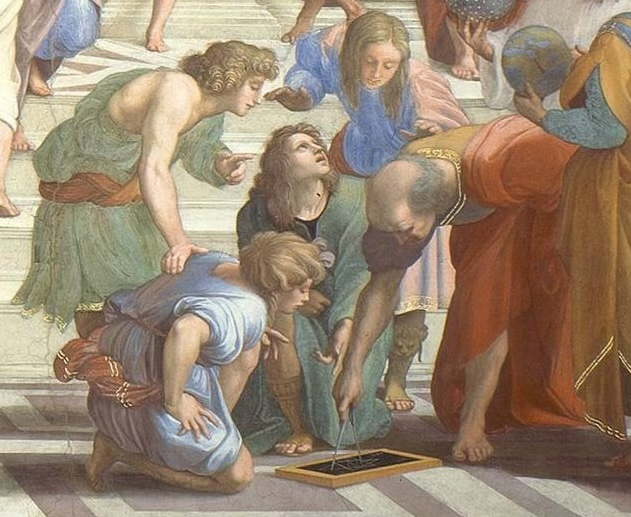
\includegraphics[scale=0.35]{img/euclid-soa}
 \caption{拉斐尔《雅典学院》局部,湿壁画,位于梵蒂冈签字厅}
 \label{fig:euclid-soa}
\end{figure}

在《原本》中,欧几里得甚至把尺规作图以公设确定下来:
\begin{enumerate}[(公设1)]
\item 过两点可作一条直线。(直尺)
\item 一条有限的直线可继续延长。(直尺)
\item 以任意点为心及任意的距离可以画圆。(圆规)
\end{enumerate}

从$\sqrt{2}$开始,古希腊人利用尺规作图和勾股定理(毕达哥拉斯定理)找出了一系列无理数。任给一条线段$AB$,规定其长度为1,用圆规在直线上依次截取长为$AB$的线段$n$次就得到了长为$n$的线段。然后在其一端作垂线(见\cref{qn:perp-of-point}),并截取出长为$m$的线段。最后连接两条相互垂直的线段端点,就得到了直角三角形。根据勾股定理,斜边长度为$\sqrt{n^2 + m^2}$(见\cref{fig:rt-mn})。当$m = n = 1$时,古希腊人就作出了$\sqrt{2}$,当$m=1, n=2$时,古希腊人就作出了$\sqrt{5}$。

\begin{figure}[htbp]
  \centering
  \subcaptionbox{直角边为$n$和$m$的三角形\label{fig:rt-mn}}{
    \begin{tikzpicture}[scale=0.8]
      \draw (0,0) -- (7,0) -- (0,4) -- cycle;
      \node[below] at (3.5,0) {$n$};
      \node[left]  at (0,2) {$m$};
      \node[above, sloped] at (3.5,2.5) {$\sqrt{m^2 + n^2}$};
      \draw[thick] (0.1,0) -- (0.1,0.1) -- (0,0.1);
    \end{tikzpicture}
  }\subcaptionbox{直角边为1和2的三角形\label{fig:rt-12}}{
    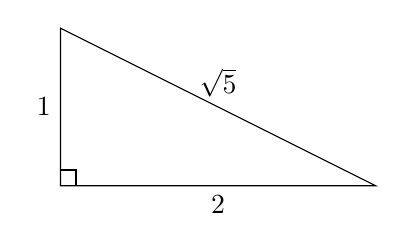
\begin{tikzpicture}[scale=2]
      \draw (0,0) -- (2,0) -- (0,1) -- cycle;
      \node[below] at (1,0) {$2$};
      \node[left]  at (0,0.5) {$1$};
      \node[above, sloped] at (1,0.5) {$\sqrt{5}$};
      \draw[thick] (0.1,0) -- (0.1,0.1) -- (0,0.1);
    \end{tikzpicture}
  }
  \caption{利用勾股定理获得无理数}
  \label{fig:irrational-tagent}
\end{figure}

这个值可不一般。我们延长$\sqrt{5}$一个单位(用圆规在斜边延长线上截取1)得到$1 + \sqrt{5}$,然后再取其一半(见\cref{qn:perp-of-point})得到$\phi = \frac{1 + \sqrt{5}}{2}$。这个值就是大名鼎鼎的黄金分割比。其十进制小数约为1.618\footnote{也叫做黄金分割数、黄金数或黄金比。中学数学课上给出的黄金比近似值是0.618,可以通过在斜边$\sqrt{5}$上截掉1,然后折半得到。}。\cref{fig:gold-ratio}是文艺复兴时期的大师达·芬奇的名作维特鲁威人。据说他正是通过研究完美的人体比例深刻认识到了黄金分割比,并且有意识地在艺术作品的构图和建筑设计中大量使用黄金比。令维特鲁威人的身高为1,腰部以下的部分为$x$,腰部以上为$1 - x$。达·芬奇认识到腰部将人体分割为两部分的比例(即$(1 - x) : x$)等于腰部以下部分与人体身高的比例(即$x : 1$),写成等式就是$(1 - x) : x = x : 1$。欧几里得在《原本》中称其为“极端与平均比率”(extreme and mean ratio)。利用比例内项积等于外项积(见第\ref{sec:frac-equiv}节)将此化为$x^2 + x - 1 = 0$,解二次方程得$x_{1, 2} = \frac{-1 \pm \sqrt{5}}{2}$。

\begin{figure}[htbp]
 \centering
 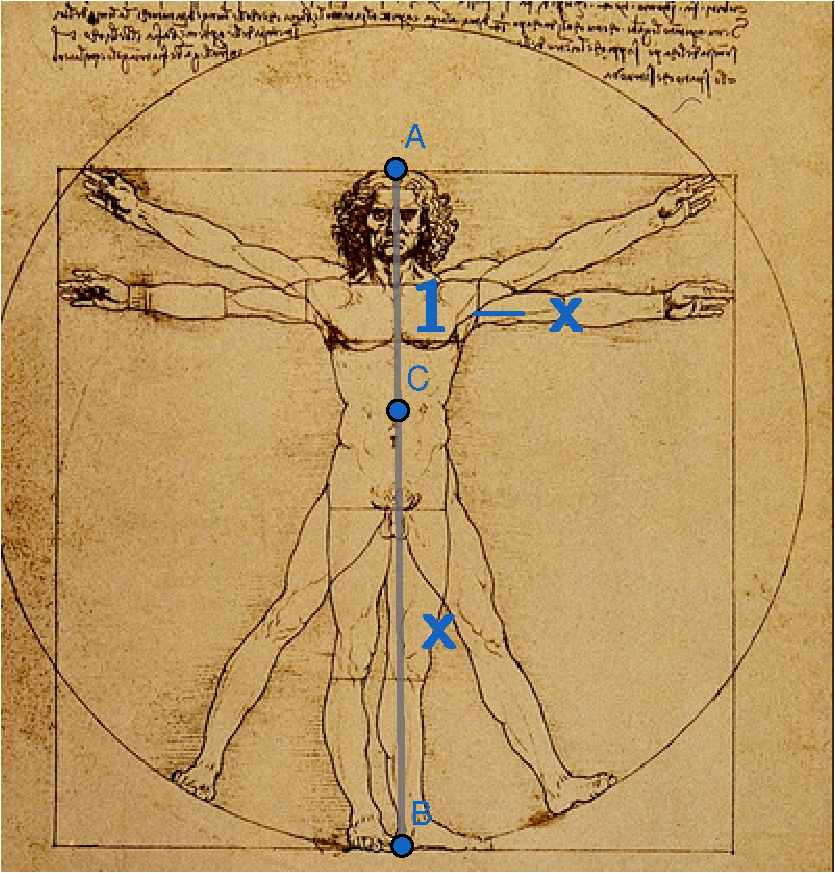
\includegraphics[scale=0.4]{img/gold-ratio}
 \caption{达·芬奇的素描维特鲁威人,1490年}
 \label{fig:gold-ratio}
\end{figure}

由于\cref{fig:gold-ratio}中的$x < 1$,故取$x = \frac{\sqrt{5} - 1}{2} \approx 0.618$。如果令腰部以上的部分为1,腰部以下部分为$x$。同样的黄金分割——使得腰部将人体分割为两部分的比例(即$1 : x$)等于腰部以下部分与人体身高的比例(即$x : (1 + x)$),写成等式就是$1 : x = x : (1 + x)$。这导致另一个方程$x^2 - x - 1 = 0$,解此二次方程得$x_{1, 2} = \frac{1 \pm \sqrt{5}}{2}$。这里由于$x > 0$,故取$x = \frac{1 + \sqrt{5}}{2} \approx 1.618$。注意到这两个值互为倒数:

\[
\frac{\sqrt{5} - 1}{2} \times \frac{\sqrt{5} + 1}{2} = \frac{(\sqrt{5})^2 - 1}{4} = \frac{5 - 1}{4} = 1
\]

所以我们在提到黄金比时,$\phi = \frac{\sqrt{5} \pm 1}{2}$都正确,要取决于上下文的具体含义(见\cref{fig:2-cases-phi})。我们接下来证明黄金数是一个无理数。

\begin{figure}
  \centering
  \subcaptionbox{$\phi = \frac{\sqrt{5} - 1}{2} \approx 0.618$}{
    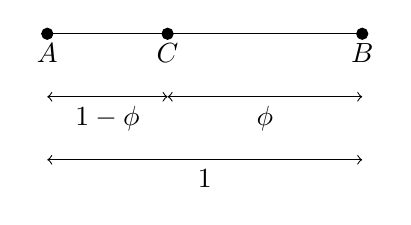
\begin{tikzpicture}[scale=4]
        \pgfmathsetmacro{\a}{0.382}

        \draw (0,0) -- (1,0);

        \filldraw (0,0) circle (0.5pt) node[below] {$A$};
        \filldraw (\a,0) circle (0.5pt) node[below] {$C$};
        \filldraw (1,0) circle (0.5pt) node[below] {$B$};

        \draw[<->] (0,-0.2) -- (\a,-0.2) node[midway,below] {$1-\phi$};
        \draw[<->] (\a,-0.2) -- (1,-0.2) node[midway,below] {$\phi$};
        \draw[<->] (0,-0.4) -- (1,-0.4) node[midway,below] {$1$};
    \end{tikzpicture}
  }\subcaptionbox{$\phi = \frac{\sqrt{5} + 1}{2} \approx 1.618$}{
    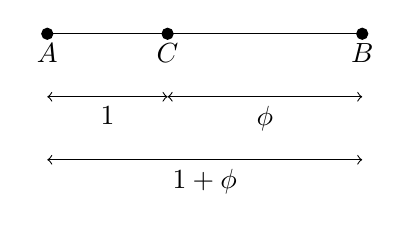
\begin{tikzpicture}[scale=4]
        \pgfmathsetmacro{\a}{0.382}

        \draw (0,0) -- (1,0);

        \filldraw (0,0) circle (0.5pt) node[below] {$A$};
        \filldraw (\a,0) circle (0.5pt) node[below] {$C$};
        \filldraw (1,0) circle (0.5pt) node[below] {$B$};

        \draw[<->] (0,-0.2) -- (\a,-0.2) node[midway,below] {$1$};
        \draw[<->] (\a,-0.2) -- (1,-0.2) node[midway,below] {$\phi$};
        \draw[<->] (0,-0.4) -- (1,-0.4) node[midway,below] {$1 + \phi$};
    \end{tikzpicture}
  }
  \caption{黄金分割的两种含义}
  \label{fig:2-cases-phi}
\end{figure}


\begin{proof}
用反证法,假设黄金数$\phi = \frac{a}{b}$可以写成即约分数,其中$b \ne 1$。它满足方程$\phi^2 \pm \phi - 1 = 0$,代入$\frac{a}{b}$:
\begin{align*}
(\frac{a}{b})^2 & = 1 \pm \frac{a}{b}  \\
a^2 &= b^2 \pm ab && \text{两边乘以}b^2 \\
a^2 &= b(b \pm a)
\end{align*}
因为$a, b$互素,它们不可能都是偶数。如果$a$是奇数$b$是偶数,则左边$a^2$是奇数,但右边是偶数导致矛盾;如果$a$是偶数$b$是奇数,则左边$a^2$是偶数,但右边的$b \pm a$是奇数,乘以奇数$b$还是奇数,也导致矛盾;如果$a, b$都是奇数,则左边$a^2$是奇数,但右边$b \pm a$是偶数,所以右边的值是偶数,仍然矛盾。故假设错误,黄金数是无理数。
\end{proof}

还记得希帕索斯传说的另一个版本么?毕达哥拉斯学派的五角星徽章标志包含着无理数。这个无理数恰好就是黄金分割数$\phi$。我们接下来揭示这个神秘的联系。这一方法来自洛克哈特的《度量》一书。

\begin{figure}[htbp]
 \centering
 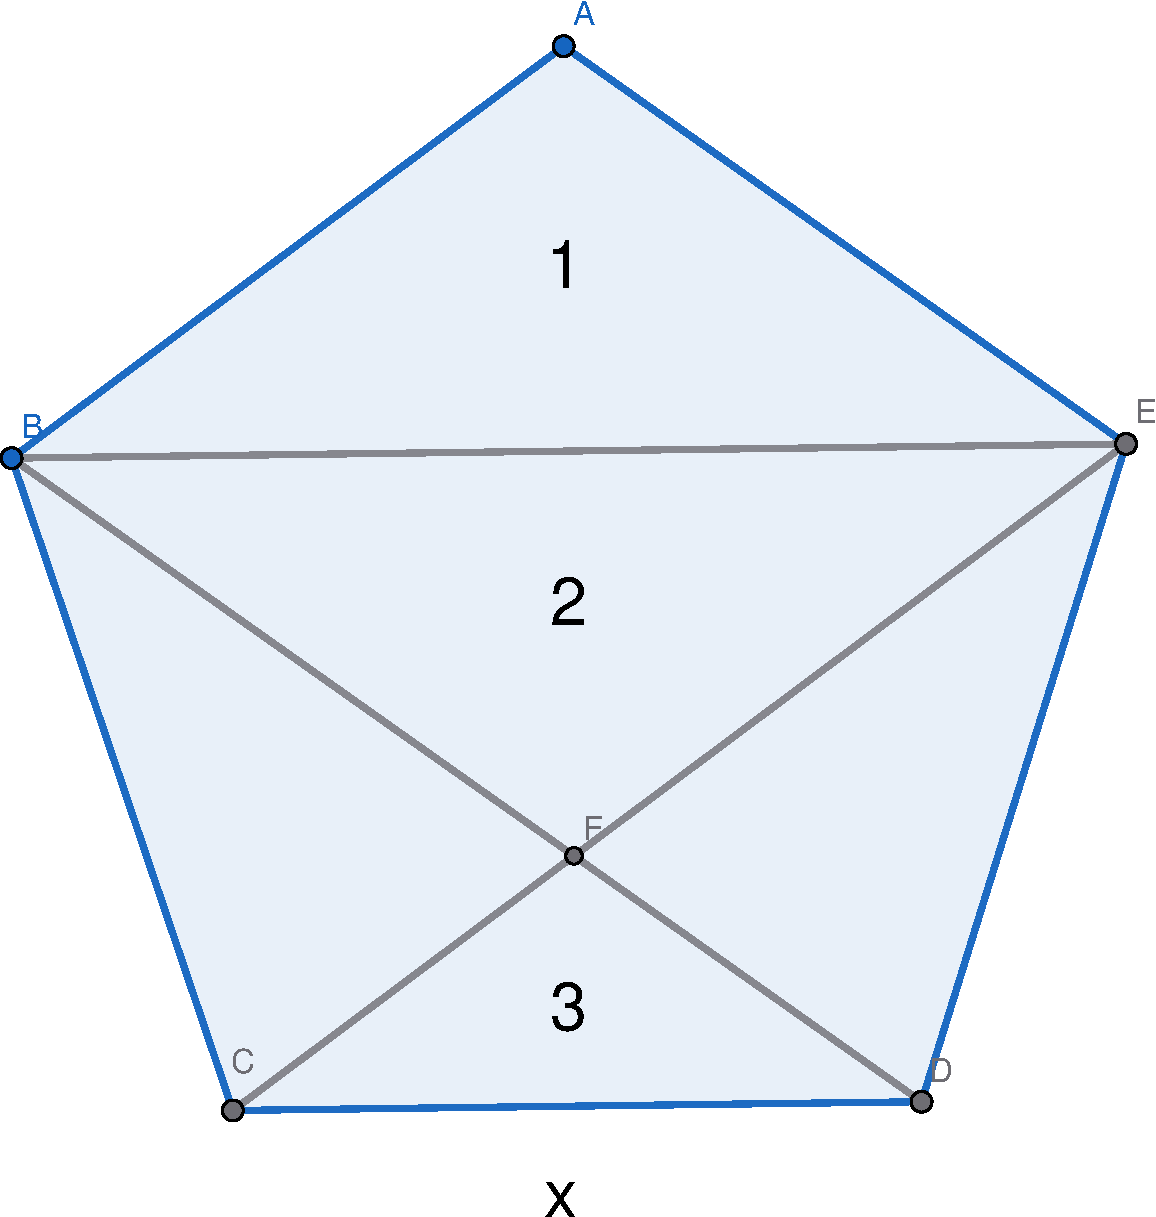
\includegraphics[scale=0.3]{img/pentagon}
 \caption{正五边形}
 \label{fig:pentagon}
\end{figure}

\label{sec:pentagon-edge}
观察\cref{fig:pentagon}中的正五边形,三角形1和2全等,2和3相似(我们略去了详细的证明,不难看出1、2都是等腰三角形,有一公共边,底角都是36度。2、3是有对顶角的等腰三角形)。令对角线$BE$的长度为1,正五边形的边长为$x$,由于三角形1和3相似,所以:

\begin{align*}
\frac{x}{1} &= \frac{AB}{BE} = \frac{FC}{CD} && \text{1, 3相似} \\
            &= \frac{EC - EF}{CD} = \frac{BE - AB}{CD} && BEC\text{是等腰三角形且1, 2全等} \\
            &= \frac{1-x}{x}
\end{align*}

这样就得到方程$x^2 + x - 1 = 0$,它的解恰恰就是黄金分割比$\phi = \frac{\sqrt{5} - 1}{2}$。在毕达哥拉斯学派的徽标中,若五角星的对角线长1,则五角星的邻角距离是$\phi$,五角星的每个角的边长是$1 - \phi$。

\index{斐波那契数列}
文艺复兴以来,黄金分割数逐渐被神秘化,引发了众多的传说,诸如:众多古希腊、古罗马的艺术作品和建筑使用了黄金数,最典型的如雅典的帕特农神庙。达·芬奇的作品如蒙娜丽莎、圣母与圣安妮等都符合黄金分割比。长宽比等于黄金比的矩形是所有矩形中最美的,以至于照片,纸张,书本都采用了黄金比的尺寸。更有甚者说:黄金比隐藏在自然万物中,鹦鹉螺的螺壳按照黄金比生长,向日葵的种子,植物的叶子,西兰花的花序都符合黄金比。种种这些说法,越传越神秘,甚至出现在小说和影视作品中(如《达·芬奇密码》)。要想破除这些数字迷信,就需要我们的老朋友——斐波那契登场了。斐波那契在《算盘书》中给出了一个问题:兔子在出生两个月后,就有繁殖能力,一对兔子每个月能生出一对小兔子来。如果所有兔子都不死,那么一年以后可以繁殖多少对兔子?开始时有一对兔子。第一个月小兔尚未具备繁殖能力,所以仍然只有一对兔子。第二个月它们生下一对小兔,共有两对。第三个月大兔子又生下一对小兔,而上月生的小兔还在成长,总共有2+1=3对。第四个月有两对大兔子产下两对小兔,加上原有的三对兔子,总共有3+2=5对(见\cref{fig:Fibonacci-rabbits})。按照这样,我们可以得到一个序列

1, 1, 2, 3, 5, 8, 13, 21, 34, 55, 89, 144, ...

\begin{figure}[htbp]
 \centering
 \subcaptionbox{正方形的边长组成了斐波那契序列\label{fig:fibonacci-spiral}}[0.45\linewidth]{
     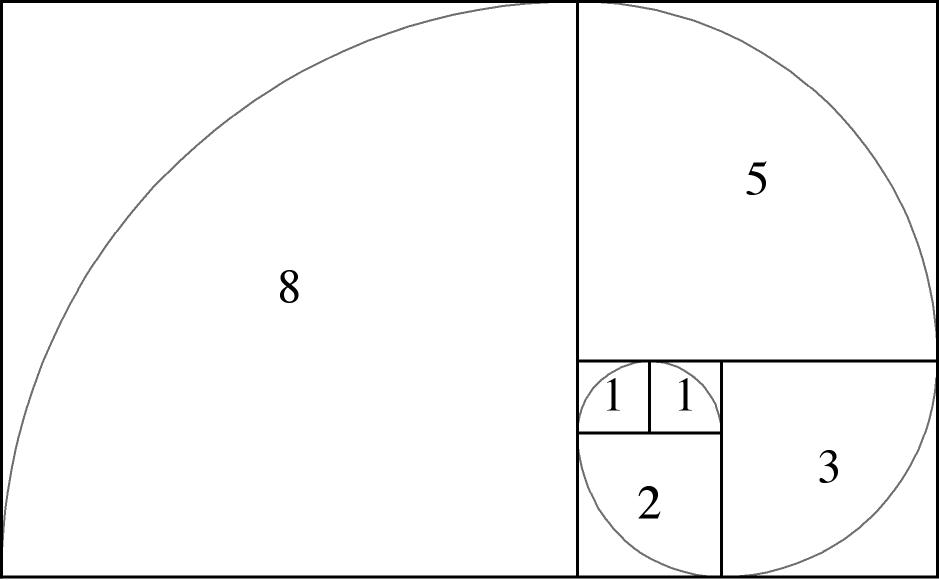
\includegraphics[scale=0.4]{img/fibonacci_spiral}}
 \subcaptionbox{黑色:成兔,白色:小兔\label{fig:Fibonacci-rabbits}}[0.45\linewidth]{
     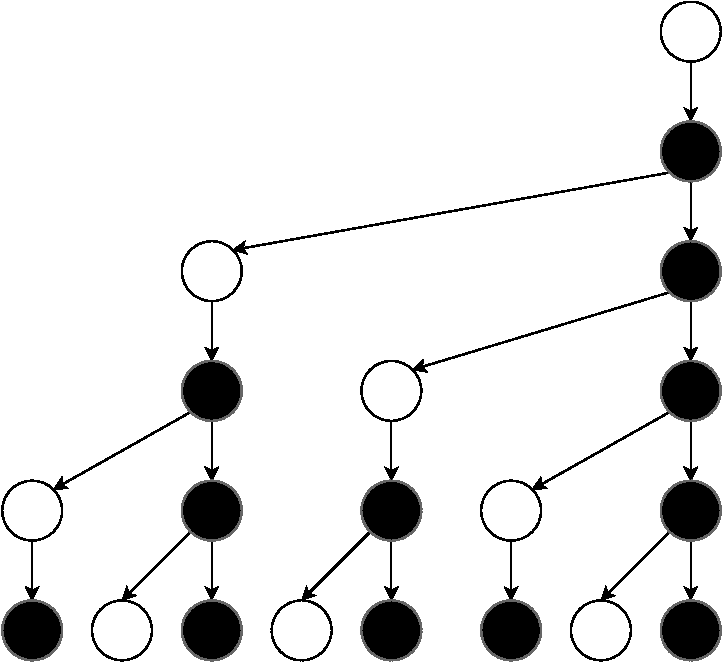
\includegraphics[scale=0.4]{img/Fibonacci-rabbits}}
 %\captionsetup{labelformat=empty}
 \caption{斐波那契序列展开}
\end{figure}

这个数列被称做斐波那契数列。它很有规律,从第三项后,任何一项都等于前两项的和。我们可以这样思考它的原理,如果前一个月有$m$对兔子,这个月有$n$对兔子,那么增加的一定都是新产下的小兔,共有$n-m$对,而剩下的都是成年兔子,共$m$对。到下个月时,这$n-m$对小兔刚刚成熟,而$m$对成兔又产下了$m$对小兔。所以下个月的兔子总数等于小兔加上成兔为:$(n - m) + m + m = n + m$对。根据这一推理,我们可以给出斐波那契数列的递归定义:

\begin{lalign}
F_0 &= 0 \\
F_1 &= 1 \\
F_{n+2} &= F_n + F_{n+1}
\end{lalign}

通常将斐波那契数列的起始值定义为0和1\footnote{如果起始值是1和3,我们就得到了卢卡斯数列1, 3, 4, 7, 11, 18, ...}。\cref{fig:fibonacci-spiral}给出了斐波那契数列的几何意义。从两个单位正方形(边长为1)开始,把它们拼成矩形。这个矩形的宽为1,长为1+1=2。把这个矩形和边长为2的正方形拼到一起,得到一个宽为2,长为2+1=3的矩形。接下来把这个矩形再和边长为3的正方形拼到一起得到宽为3,长为5的矩形。重复这一步骤,我们总可以把一个宽为$F_{n-2}$,长为$F_{n-1}$的矩形和一个边长为$F_{n-1}$的正方形拼在一起,得到一个宽$F_{n-1}$长为$F_n = F_{n-1} + F_{n-2}$的矩形。如果把每个正方形的内切1/4圆弧连起来,就得到了一个螺线,称为斐波那契螺线。

斐波那契数列增加的非常快,兔子几乎是按照指数爆炸的速度疯狂繁殖,1年后从一对变成了144对。我们知道等比数列是指数爆炸的,每一项都是前一项的固定倍数。说斐波那契数列“几乎”是指数爆炸究竟是什么意思呢?显然每一项与前一项的比不是一个固定倍数,\cref{tab:fibonacci-ratios}列出了斐波那契数列相邻项的比值。

\begin{table}[ht]
    \centering
    \begin{tabular}{|c|c|l||c|c|l|}
        \hline
        $n$ & $F_n$ & $F_n/F_{n-1}$ & $n$ & $F_n$ & $F_n/F_{n-1}$\\
        \hline
        2 & 1 & 1 &         11 & 89   & 1.6181818182 \\
        3 & 2 & 2 &        12 & 144  & 1.6179775281 \\
        4 & 3 & 1.5 &        13 & 233  & 1.6180555556 \\
        5 & 5     & 1.667 &        14 & 377  & 1.6180257511 \\
        6 & 8     & 1.6 &         15 & 610  & 1.6180371353 \\
        7 & 13    & 1.625 &         16 & 987  & 1.6180327869 \\
        8 & 21    & 1.6153846154 &        17 & 1597 & 1.6180344478 \\
        9 & 34    & 1.6190476190 &        18 & 2584 & 1.6180338134 \\
        10 & 55   & 1.6176470588 &        19 & 4181 & 1.6180340557 \\
           &      &              &        20 & 6765 & 1.6180339632 \\
        \hline
    \end{tabular}
    \caption{斐波那契数列相邻项比值}
    \label{tab:fibonacci-ratios}
\end{table}

虽然不是等比数列,但相邻项的比值越来越接近,小数点后四位稳定在1.6180。用计算器计算黄金比例$\phi = \frac{1+\sqrt{5}}{2} \approx 1.6180339887$,这与$F_{20}/F_{19}$的小数点后7位完全一样。这难道仅仅是巧合么?

\begin{proposition}
若斐波那契数列相邻项的比值收敛,则其极限为黄金分割数$\phi$。
\end{proposition}

注意这个命题没有断定一定有极限,而是说\underdot{如果}有的话,那么一定是$\phi$。证明极限存在需要高等数学的相关知识,但使用中学数学中的二次方程已经能够破解神秘的问题了。

\begin{proof}
根据斐波那契数列的递归关系:$F_n = F_{n-1} + F_{n-2}$,两边同时除以$F_{n-1}$得:

\[
\frac{F_n}{F_{n-1}} = 1 + \frac{F_{n-2}}{F_{n-1}}
\]

如果斐波那契数列相邻项的比收敛于$x$,即当$n$越来越大$n \to \infty$时,$\frac{F_n}{F_{n-1}}$和$\frac{F_{n-1}}{F_{n-2}}$都趋近$x$,那么上式趋近:

\begin{align*}
x = 1 + \frac{1}{x}  \\
x^2 - x + 1 = 0 && \text{两边乘以}x
\end{align*}
这恰恰是黄金分割数满足的方程,解方程并舍弃负根得$x = \frac{\sqrt{5} + 1}{2} = \phi$。
\end{proof}

再加上一点点理性思维,我们就能破解数字迷信了。自然界中的生物,如果在原有基础上生长,就会满足斐波那契数列。例如鹦鹉螺的螺壳,在第$n$个生长周期中,原有的部分$F_{n-1}$不会消失,并且在这个基础上又增长到$F_n$,下一个生长周期就会在$F_{n-1}$和$F_{n}$的基础上继续生长成$F_{n+1} = F_{n} + F_{n-1}$。这恰恰是斐波那契数列,所以鹦鹉螺的壳如同\cref{fig:fibonacci-spiral}那样的螺线。而这个螺线的外切矩形的长宽比为$F_{n}/F_{n-1}$,近似于并逐渐趋近于黄金比。同样的道理,\cref{fig:sunflower}中的种子在原有的基础上生长,也构成斐波那契数列。其生长轨迹是斐波那契螺线,其外切矩形的长宽比近似并趋近黄金比。这一模式在自然界中是如此普遍,这就解释了为何叶子、花序、种子、螺壳等等都呈现着斐波那契数列和黄金比。

\begin{figure}[htbp]
 \centering
 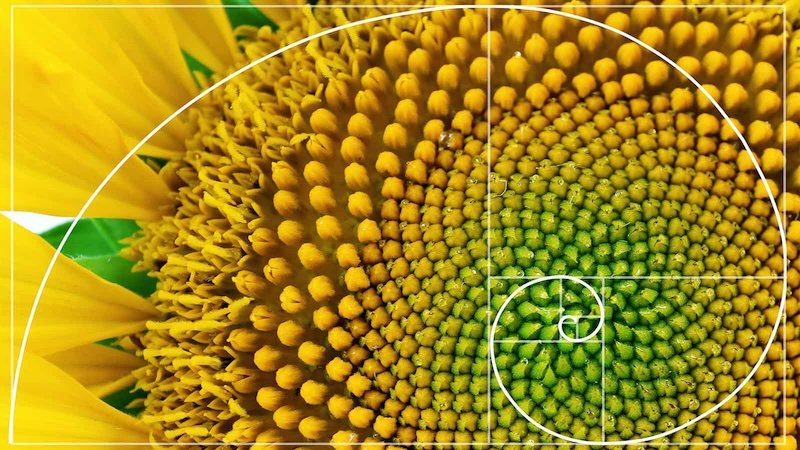
\includegraphics[scale=0.3]{img/sunflower}
 \caption{向日葵的种子按照斐波那契数列生长}
 \label{fig:sunflower}
\end{figure}

最后一个需要破除的传言是纸张的尺寸符合黄金分割比。\cref{fig:ISO216}是国际标准化组织(ISO)制定的A系列和B系列纸张尺寸。分别以国际单位制毫米(mm)和英制单位英寸(in)标注。我们熟悉的A4打印纸的尺寸为$210 \times 297$平方毫米,长宽比为$297/210 = 1.41429$,不等于黄金比1.618。B0纸张的长宽比是$1414/1000 = 1.414$。这些纸张的长宽比看似是一样的。而1.414接近$\sqrt{2}$,古希腊人发现的第一个无理数,边长为1的正方形的对角线。这是巧合么?我们只要了解ISO制定的纸张尺寸原理就能利用初中几何和方程找到答案了。为了生产方便,ISO标准定义A0的大小是1平方米,A0对折剪裁就得到两张A1,它们同A0的形状一样;一张A1对折剪裁就得到两张A2,它们的形状也一样,以此类推。同样一张B0对折剪裁得到两张B1,一张B1对折剪裁得到两张B2,以此类推,并且它们的形状都一样。我们从初中几何中立即得出,所有A系列的纸张是\underdot{相似}的矩形,所有B系列的纸张也是相似的矩形。那么什么长宽比能满足这个方便剪裁的需求呢?我们假设矩形长$r$,宽$1$(例如B0纸),对折后剪裁成两张宽$\frac{r}{2}$,长$1$的小矩形(例如两张B1纸)。由于图形相似,所以:

\begin{figure}[htbp]
 \centering
 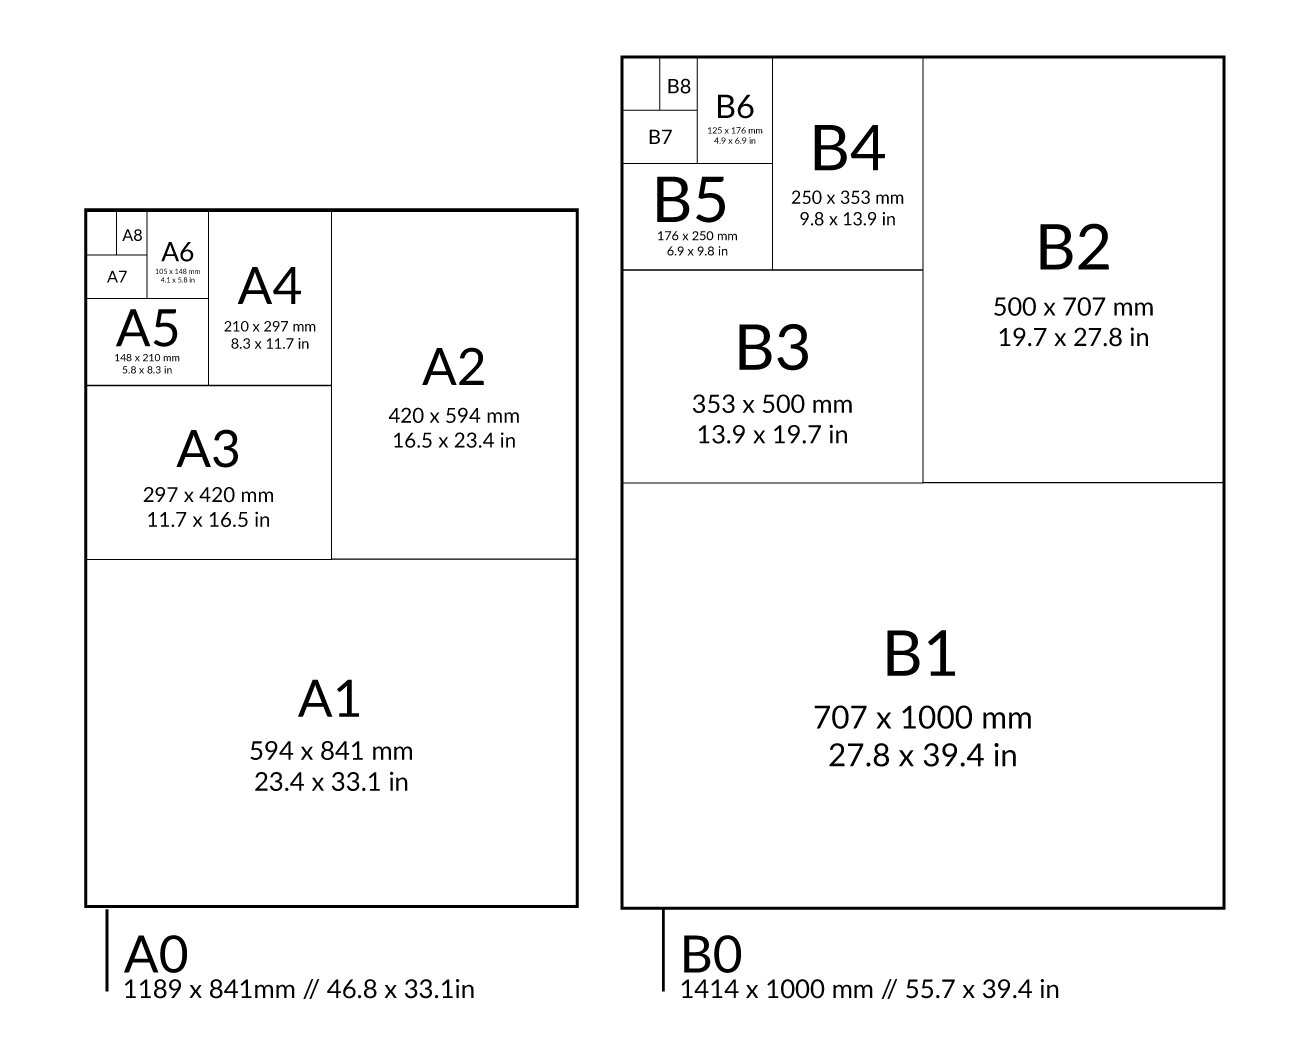
\includegraphics[scale=0.25]{img/ISO216}
 \caption{国际标准化A系列和B系列纸张尺寸}
 \label{fig:ISO216}
\end{figure}

\begin{align*}
r : 1 &= 1 : \frac{r}{2}  && \text{图形相似} \\
1 &= \frac{r^2}{2} && \text{内、外项积相等} \\
r^2 &= 2
\end{align*}

开方得$r = \sqrt{2}$。这就说明了为何国际标准的纸张长宽比必然是无理数$\sqrt{2}$。由于这个数是无理数,化成小数是无限不循环的。经过四舍五入和单位转换就出现了精度损失。例如$B5$的长宽比为$250/176 = 1.42$。我们甚至能自己推出A0的尺寸:由于A0的面积是1平方米,令其宽为$a$,长为$a\sqrt{2}$,面积$s = a^2\sqrt{2} = 1$,解方程得$a = \sqrt{\frac{1}{\sqrt{2}}} \approx 0.841$米。长为$1 / 0.841 = 1.189$米,和\cref{fig:ISO216}完全一样。同时我们也立即知道了B系列的定义: B0的尺寸为$\sqrt{2}$平方米。所以每个$B$系列的尺寸是对应$A$系列尺寸的$\sqrt{2}$倍。我们甚至可以进一步推测:建筑的瓷砖如果易于切割,产生相似的矩形,则它们也必然满足$\sqrt{2}$的长宽比。这样我们就破除了谣言和迷信,而回归了科学和理性。也许你觉得这太不浪漫了,缺少了神秘感。但这样的推理过程本身是优美的,我们解开了大自然和人类自己生产劳动的内在规律,这些规律同样是和谐的,是美的,是浪漫的。

作为本节的结束,我们摘录一段我国伟大的数学家华罗庚先生的“最后的演讲”\footnote{1985年6月12日下午,74岁的华罗庚在日本东京大学理学部作题为《理论、应用与普及》的演讲。演讲完毕后,他在热烈的掌声中走向轮椅,但不幸倒在地上。因心脏病突发,华罗庚于当日晚十时去世\citepage[21页]{ZhangJianan-2017}。}。

\begin{quotation}
如果说我到车间去讲优选法,要求听讲的工人都要学过微积分,这是不可能的。那么我是怎么在中国普及优选法的呢?首先我让大家记住一个数 ——0.618。这张纸条和这支烟就是我的教具。假定纸条就代表某一因素的范围。第一个试验在什么地方做呢?在全长的 0.618 处做。(此时华老点燃了烟,用烟头在纸条的 0.618 处烧了一个洞)第二个试验点又在什么地点做呢?在纸上第一个试验点的对称点上做,在我这里就很简单地找到了。把纸对折起来,顺着第一个试验点所烧的洞烧过去,第二个试验点就得到了。这时,可将两个试验点所得到的结果对比一下,看哪个试验点所出的效果好?如果第一点比第二点好,那么就把第二点以下撕掉;如果第二点比第一点好,第一点以上已经被撕掉了。下一个试验在什么地点作呢?仍然是把剩余的纸条对折一下,顺着剩下的试验点所烧的洞烧过去,就得到了第三个试验点。然后再作比较,留下好的,撕去坏的。以后怎么做,不用我讲了吧!(笑声)一直作到生产上所需要的精度为止。(《华罗庚诗文选》)
\end{quotation}

\section{欧几里得算法}

古希腊人认识到新发现的这一类数与此前的数不同。首先,它们是客观存在的,通过尺规作图作图可以实实在在地构造出来。其次,它们不能表达为整数或者整数的比。为了把它们归入数的大家庭,人们需要解决一系列问题:(1) 如何区分和定义这一类数?(2) 如何认识、衡量它们的大小?(3) 它们在数轴上的位置是什么?(4) 尽管它们不能表示为即约分数,有没有办法用分数逼近它们?经过欧多克索斯和欧几里得之手,和这些问题引出了丰硕的成果。

我们在前面的尺规作图中,通常先把一个给定的线段定义为1,然后动手延长截取出$n$。这个被定义为1的线段相当于一把尺子,用它可以度量出长度为$n$的线段。毕达哥拉斯学派为了将几何纳入“万物皆数”的理论,提出了一个概念来定义一条线段可以用另一条线段来度量。这个定义说,如果一条线段A可以通过有限个另一条线段V来表示时,称线段V可用作线段A的量度(measure)。这本质上是说,我们可以通过整数次拼接产生另一条线段。尽管度量两条不同的线段时,可以使用各自的量度,但是如果想用同一量度测量不同的线段,它必须是二者的公度(common measure)。即当且仅当线段V可以同时成为线段A和线段B的量度时,它才能成为二者的公度。“万物皆数”用公度的概念来解释就是万物彼此间都可以找到公度。

\index{最大公度}
由于公度可能有多个,为此需要引入\underdot{最大}公度\footnote{英文greatest common measure简称gcm,线段的长度是整数时,通常称最大公约数,英文为greatest common divisor,简称gcd}的概念。如果线段V是线段A和线段B的公度,并且比其它公度都大,则称V是A和B的最大公度。已知两条线段,怎样才能求得最大公度呢?这就引出了历史上著名的递归算法——欧几里得算法(又称辗转相除法)\footnote{印度和中国分别独立发现了欧几里得算法。五世纪末,印度数学家阿耶波多(Aryabhata)用这一算法解不定方程(丢番图方程)。在《孙子算经》中,欧几里得算法可以作为中国剩余定理的特例。在1247年,南宋数学家秦九韶在《数书九章》中详细给出了欧几里得算法。}。在欧几里得《原本》卷十命题3中\cite{Elements},详细阐述了这一算法\footnote{在《原本》卷七的命题1中,有针对整数的欧几里得算法。但针对线段的情形实际上覆盖了整数。}。

\index{欧几里得算法}
\begin{proposition}[《原本》,卷十,命题3]
已知两个可公度的量,求它们的最大公度量。
\end{proposition}

第\ref{sec:gcd-minus}节中,我们介绍了欧几里得算法的减法形式求两个自然数的最大公约数。《原本》将其从自然数扩展到几何量,从而更加通用。欧几里得给出的方法,只需要使用递归和减法。因此本质上可以用尺规作图的方式求出最大公度。我们再次把这一算法的形式化定义列出:

\[
(a, b) = \begin{cases}
  a > b :& (a - b, b) \\
  a = b :& a \\
  a < b :& (a, b - a)
  \end{cases}
\]

设两条线段$a$、$b$可公度,如果它们相等,则最大公度就是其中的任一条线段,此时算法返回$a$作为结果。如果线段$a$比$b$长,就用圆规\underdot{不断}从$a$中截去$b$(通过递归),然后求截短的线段$a'$和$b$的最大公度;否则如果线段$b$比$a$长,就反过来\underdot{不断}从$b$中截去$a$,然后求$a$和截短的线段$b'$的最大公度。\cref{fig:line-seg-gcm}描述了这一算法作用于两条线段的计算步骤。我们也可将这一算法应用于整数42和30并与处理线段的过程进行对比:

\[
(42, 30) = (12, 30) = (12, 18) = (12, 6) = (6, 6) = 6
\]

\begin{figure}[htbp]
  \centering
  \begin{tikzpicture}[scale=0.125]
    \filldraw (0, 0) circle (0.5)   (30, 0) circle (0.5)   (42, 0) circle (0.5);
    \draw (-8, 0) node{$a$} (0, 0) -- (42, 0);
    \filldraw (0, -5) circle (0.5)   (30, -5) circle (0.5);
    \draw (-8, -5) node{$b$} (0, -5) -- (30, -5);

    \filldraw (0,  -15) circle (0.5)   (12, -15) circle (0.5);
    \draw (-8, -15) node{$a'=a-b$} (0, -15) -- (12, -15);
    \filldraw (0, -20) circle (0.5)   (12, -20) circle (0.5)   (24, -20) circle (0.5)   (30, -20) circle (0.5);
    \draw (-8, -20) node{$b$} (0, -20) -- (30, -20);

    \filldraw (0,  -30) circle (0.5)   (6, -30) circle (0.5)   (12, -30) circle (0.5);
    \draw (-8, -30) node{$a'$} (0, -30) -- (12, -30);
    \filldraw (0, -35) circle (0.5)   (6, -35) circle (0.5);
    \draw (-8, -35) node{$b'=b-2a'$} (0, -35) -- (6, -35);

    \filldraw (0,  -45) circle (0.5)   (6, -45) circle (0.5);
    \draw (-8, -45) node{$a''=a'-b'$} (0, -45) -- (6, -45);
    \filldraw (0, -50) circle (0.5)   (6, -50) circle (0.5);
    \draw (-8, -50) node{$b'$} (0, -50) -- (6, -50);
  \end{tikzpicture}
  \caption{欧几里得算法的线段示意}
  \label{fig:line-seg-gcm}
\end{figure}

\subsection{改进欧几里得算法}
将$b$反复从$a$中减去,最后得到$a'$的过程恰好是带余数除法的定义,即$a' = a - qb$,其中$q$是商,$a'$相当于余数。我们把这个取余数的过程记为$a'= a \bmod b$,并用除法和求余数运算代替原始欧几里得算法中的反复相减(用圆规截去)。此外,当一个量是另一个量的整倍数时,例如$b \leq a$且$b$可以整除$a$,我们立即知道最大公度为$b$。此时求余数的结果$a \bmod b = 0$,为此可以定义$(0, b) = (b, 0) = b$。我们可以先比较$a$和$b$的大小,如果$a < b$就交换两个量。由于我们知道$a \bmod b$一定小于$b$, 所以下次递归时可以直接交换为$(b, a \bmod b)$。这样就得到了改进的欧几里得算法:

\be
(a, b) = \begin{cases}
  a < b: & (b, a) \\
  b = 0: & a \\
  a > b: & (b, a \bmod b)
\end{cases}
\label{eq:gcm}
\ee

\begin{proof}
为什么这个算法可以求出最大公度呢?我们分两步证明它的正确性:第一步证明这一算法可以求出公度;第二步证明求出的公度是最大的。设$b \leq a$(否则交换$a, b$),利用带余数除法求$a$除以$b$。令整数$q_0$为商(从线段$a$中用圆规截去$b$的次数),$r_0$为余数(截去后剩余的线段),即$a = b q_0 + r_0$。如果$r_0$为零,就找到了公度(截去后无剩余,线段$b$可以量尽$a$),为此我们只需要考虑$r_0$不为零的情况。继续用带余数除法:$b = r_0 q_1 + r_1$,类似地,只要余数不为零,可以一直列出这样的式子:

\begin{align*}
a   &= b q_0 + r_0 \\
b   &= r_0 q_1 + r_1 \\
r_0 &= r_1 q_2 + r_2 \\
r_1 &= r_2 q_3 + r_3 \\
    & \cdots
\end{align*}

但只要$a$、$b$是可公度的,这些式子就不会无限列下去。因为商是整数(用圆规截取整数次),并且余数总小于除数,即:$b > r_0 > r_1 > r_2 > \dotsb \ge 0$。但余数不可能小于零,而起始值是有限的,所以最终一定在有限步内得到:

\begin{salign}
       & \cdots \\
r_{n-1} &= r_n q_{n+1}
\label{eq:termination-of-euclidean-algorithm}
\end{salign}

接下来我们证明最后得到的$r_n$可以同时度量$a$和$b$。根据度量的定义和\cref{eq:termination-of-euclidean-algorithm},显然$r_n$可以度量$r_{n-1}$。然后考虑倒数第二式$r_{n-2} = r_{n-1} q_n + r_n$。由于$r_n$可以度量$r_{n-1}$,所以$r_n$也可以度量$r_{n-1} q_n$,自然它也可以度量$r_{n-1} q_n + r_n$,这个量恰好就是$r_{n-2}$。以此类推向上逐一证明$r_n$可以度量$r_{n-1}, r_{n-2}, \dotsc, b, a$。这样就证明了欧几里得算法得到的答案$r_n$是$a$和$b$的公度。

第二步我们要证明$r_n$是最大公度,即任何$a$和$b$的公度$c$也可以度量$r_n$。由于$c$是公度,因此$a$和$b$是它的整数倍。记$a = mc, b = nc$,其中$m, n$都是整数。代入$a = b q_0 + r_0$得$mc = ncq_0 + r_0$。移项得$r_0 = (m - nq_0)c$,因此$c$也可以度量$r_0$。以此类推逐一证明$c$可以度量$a, b, r_0, r_1, \dotsc, r_n$。这样就证明了任何公度$c$都可以度量$r_n$,因此$r_n$是最大公度。这样就证明了欧几里得算法的正确性。
\end{proof}

我们用符号$d = r_n$表示$a, b$的最大公度。进一步,$d$还是下面每一对量的最大公度:

\be
d = (a, b) = (b, r_0) = \dotso = (r_{n-1}, r_n) = r_n
\label{eq:recursive-gcm}
\ee

\cref{fig:geometric-GCM}给出了欧几里得算法的一个几何解释。求线段$a, b$的最大公度相当于找到一块最大的方砖,可以恰好铺满长$a$,宽$b$的矩形地板。想象一张$a \times b$大小的纸,我们首先反复剪掉边长为$b$的正方形,最后得到$b \times r_0$大小的矩形纸;然后再反复剪掉边长为$r_0$的正方形,得到$r_0 \times r_1$大小的矩形;不断剪掉正方形,最后剩下的一个正方形的边长就是最大公度。我们可以用这样大小的方砖铺盘矩形地板。

\begin{figure}[htbp]
 \centering
 \subcaptionbox{反复剪掉正方形。(1) 左上:长$b$宽$a$的矩形;(2) 左下:剪掉两个边为$a$的正方形;(3) 右上:剪掉3个边为$c$的矩形;(4) 右下:剪掉4个边为$d$的矩形。}{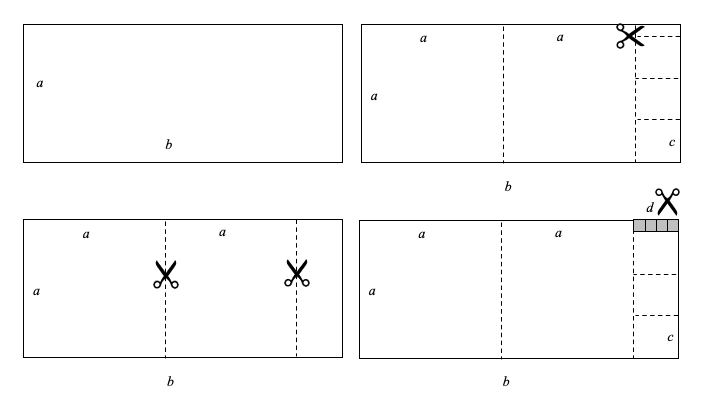
\includegraphics[scale=0.4]{img/GCM}}
 \subcaptionbox{用最终的小正方形铺满原图}{
   \begin{adjustbox}{max width=0.8\textwidth}
   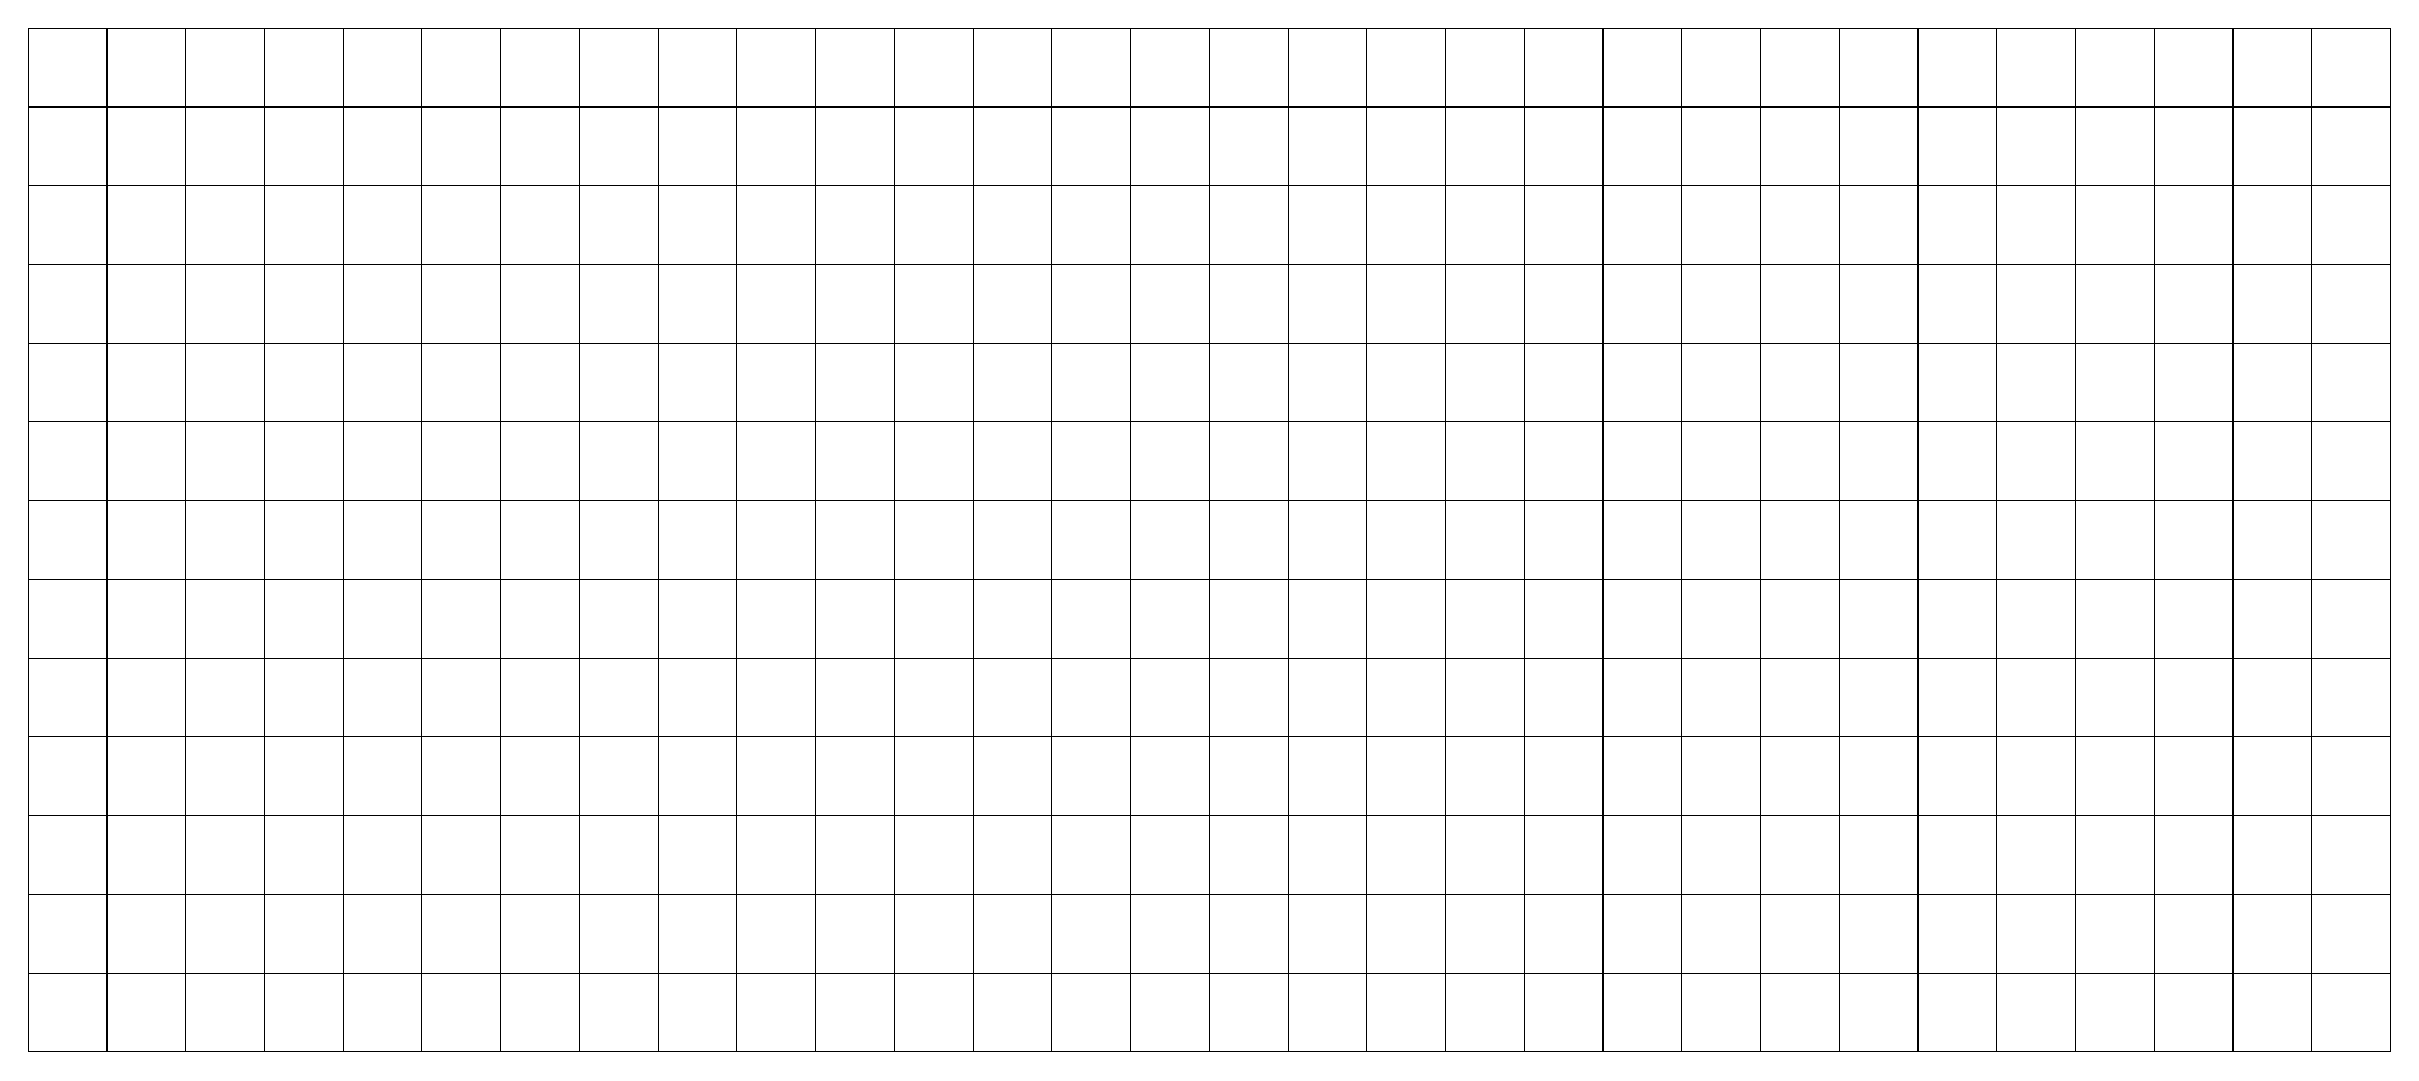
\begin{tikzpicture}
     \draw[step=1, thin] (0, 0) grid (30, 13);
   \end{tikzpicture}
   \end{adjustbox}
 }
 \caption{欧几里得算法的几何解释}
 \label{fig:geometric-GCM}
\end{figure}

\subsection{扩展欧几里得算法}
\index{扩展欧几里得算法} \index{贝祖等式}

贝祖等式\footnote{Bézout's identity,整数中的贝祖等式(或称贝祖定理,也译作裴蜀定理)最早由法国数学家梅齐里亚克证明。法国数学家贝祖证明了它对多项式也成立。在抽象代数中,贝祖等式可推广到任意主理想环上。}是欧几里得算法的一个重要结果。

\begin{figure}[htbp]
 \centering
 \subcaptionbox{贝祖(Étienne Bézout, 1730~1783年)\label{fig:Bezout}}[0.45\linewidth]{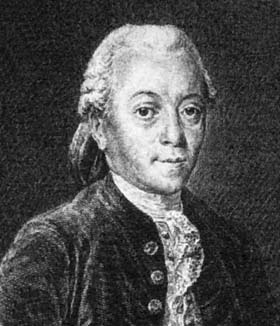
\includegraphics[scale=0.45]{img/Bezout}}
 \subcaptionbox{梅齐里亚克(Claude Gaspard Bachet de Méziriac, 1581~1638年)\label{fig:Meziriac}}[0.45\linewidth]{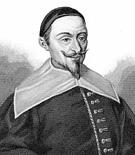
\includegraphics[scale=0.95]{img/Meziriac}}
 \caption{贝祖和梅齐里亚克}
\end{figure}

\begin{theorem}[贝祖等式]
如果$d$是$a$和$b$的最大公度,则存在整数$x$和$y$使得:

\be
ax + by = d
\label{eq:bezouts-identity}
\ee
\end{theorem}

\begin{proof}
考虑所有形如$ax + by$这样的正数(或正的线段长度)组成的集合:

\[
S = \{ ax + by \}, x, y \text{是整数,且} ax + by > 0
\]

$S$一定不为空,它至少包含$a$(此时$x = 1, y = 0$)和$b$(此时$x = 0, y = 1$)。因为$S$的所有元素都为正,所以它一定有一个最小的元素,我们将其记为$d = as + bt$。我们接下来要证明$d$就是$a$和$b$的最大公度。使用带余数的除法用$a$除以$d$:

\be
a = qd + r
\label{eq:Euclidean-division}
\ee

其中$q$是商,余数$0 \leq r < d$。余数$r$要么为0,要么在集合$S$中,这是因为:

\begin{align*}
r & = a - qd          && \text{由\cref{eq:Euclidean-division}} \\
  & = a - q(as + bt)  && \text{代入}d = as + bt \\
  & = a(1 - qs) - bqt && \text{合并整理} \\
  & = ax' + by'       && \text{令}x' = 1 - qs, y' = -bq
\end{align*}

符合集合$S$中元素的形式。但我们之前假设$d$是$S$中的最小正元素,而$r$却比$d$还小,这样就会产生矛盾。因此必定有$r = 0$。\cref{eq:Euclidean-division}就化为$a = qd$,因此$d$可以度量$a$。用同样的方法可以证明$d$也可以度量$b$。因此$d$是它们的公度。我们接下来证明$d$是最大公度。令$c$为$a$和$b$的任意公度,根据定义,存在整数$m$、$n$使得$a = mc$、$b = nc$。这样$d$就可以表示为:

\begin{align*}
d & = as + bt    \\
  & = mcs + nct  && c\text{是$a$和$b$的公度} \\
  & = c(ms + nt) && d\text{是$c$的倍数}
\end{align*}

这说明$c$可以度量$d$,也就是说$c \leq d$。这就证明了$d$是最大公度。综上我们就证明了贝祖等式,即存在整数使得$ax + by = d$,并且进一步得知最大公度是所有形如$ax + by$的正值中最小的。
\end{proof}

但如何找到具体的$x$和$y$使得$d = ax + by$呢?使用贝祖等式,我们可以推导出\underdot{扩展}欧几里得算法,同时找出最大公度和对应的$x$与$y$:

\begin{align*}
ax + by & = d = (a, b)   && \text{贝祖等式} \\
        & = (b, r_0)     && \text{欧几里得算法,\cref{eq:recursive-gcm}} \\
        & = bx' + r_0 y' && \text{对$b$和$r_0$使用贝祖等式} \\
        & = bx' + (a - bq_0)y'  && \text{由$a = b q_0 + r_0$} \\
        & = ay' + b(x' - y'q_0) && \text{整理为$a$和$b$的项} \\
        & = ay' + b(x' - y' \lfloor a / b \rfloor) && \text{将$q_0$表示为$a$与$b$的商}\lfloor a / b \rfloor
\end{align*}

这样就得出了关系:

\[
x = y' \qquad y = x' - y' \lfloor a / b \rfloor
\]

边界条件出现在$b = 0$的时候,此时最大公度$(a, 0) = 1a + 0b$。把边界条件和上述关系归纳起来就得到了扩展欧几里得算法:

\be
(a, b)' =
\begin{cases}
  a < b: & (b, a)' \\
  b = 0: & (a, 1, 0) \\
  a > b: & (d, y', x' - y' \lfloor a / b \rfloor), \text{其中}(d, x', y') = (b, a \bmod b)'
\end{cases}
\label{eq:gcm-ext}
\ee

为了和标准欧几里得算法区别,扩展算法用记号$(a, b)'$,它的结果包含3部分:$(d, x, y)$,分别是最大公度和对应的$x$与$y$。如果$a$小于$b$,就交换它们再求最大公度;如果$b = 0$,则最大公度就是a,并且$x = 1, y = 0$。此时结果为$(a, 1, 0)$;否则,我们递归地用扩展算法求$(b, a \bmod b)'$的最大公度$d$和对应的$x'$与$y'$,然后利用关系$x = y', y = x' - y' \lfloor a / b \rfloor$进一步求出$x, y$。

我们再次用42和30作为例子,应用扩展欧几里得算法求$(d, x, y) = (42, 30)'$。
\begin{enumerate}[步骤(1)]
\item 递归求$(d, x', y') = (30, 12)'$,其中12是42除以30的余数;
\item 递归求$(d, x'', y'') = (12, 6)'$,其中6是30除以12的余数;
\item 递归求$(6, 0)'$,其中0是12除以6的余数,根据边界条件$(6, 0)' = (6, 1, 0)$,即$(d = 6, x''' = 1, y''' = 0)$;
\item 返回(2)得$(d = 6, x'' = y''' = 0, y'' = x''' - \lfloor 12/6 \rfloor y''' = 1 - 2 \times 0 = 1)$;
\item 返回(1)得$(d = 6, x' = y'' = 1, y' = x'' - \lfloor 30/12 \rfloor y'' = 0 - 2 \times 1 = -2)$;
\item 最终返回得$(d = 6, x = y' = -2, y = x' - \lfloor 42/30 \rfloor y' = 1 - 1 \times (-2) = 3)$。
\end{enumerate}
最后验证:$ax + by = 42 \times (-2) + 30 \times 3 = 6 = d$,的确等于最大公度。

作为扩展欧几里得算法的应用,我们给出一道有趣的题目\citepage[23页]{LiuXinyu-2022}。有两个水瓶,容量分别是9升和4升,问如何才能从河中打出6升水?这道题目有很多变化形式,瓶子的容积和取水的容量可以是其它数值。有一个故事说解决这道题目的主人公是少年时代的法国数学家泊松(Sim\`{e}on Denis Poisson)。两个瓶子共有6种操作。记大瓶子为$A$,容积为$a$;小瓶子为$B$,容积为$b$:

\begin{itemize}
\item 将大瓶子$A$装满水;
\item 将小瓶子$B$装满水;
\item 将大瓶子$A$中的水倒空;
\item 将小瓶子$B$中的水倒空;
\item 将大瓶子$A$中的水倒入小瓶子$B$;
\item 将小瓶子$B$中的水倒入大瓶子$A$。
\end{itemize}

最后两种操作中,任意一个瓶子满或者空时就停止。\cref{tab:jug-ops}给出了一系列倒水动作的例子,这里假设容积$b < a < 2b$。

\begin{table}[htbp]
\centering
\begin{tabular}{|l|l|l|}
\hline
$A$ & $B$ & 操作 \\
\hline
0 & 0 & 开始 \\
0 & $b$ & 倒满$B$ \\
$b$ & 0 & 将$B$倒入$A$ \\
$b$ & $b$ & 倒满$B$ \\
$a$ & $2b - a$ & 将$B$倒入$A$ \\
0 & $2b - a$ & 倒光$A$ \\
$2b - a$ & 0 & 将$B$倒入$A$ \\
$2b - a$ & b & 倒满$B$ \\
a & $3b - 2a$ & 将$B$倒入$A$ \\
... & ... & ... \\
\hline
\end{tabular}
\caption{两个瓶子的水量和倒水操作的对应关系}
\label{tab:jug-ops}
\end{table}

无论进行何种操作,每个瓶子中的水的容量总可以表示为$ax + by$的形式,其中$x$、$y$是整数。根据贝祖等式的证明,水容量的最小正值就是$a$和$b$的最大公度$d$。给定两个瓶子的容量,我们立即能够判断是否可以得到体积为$c$的水——当且仅当$c$能够被$d$度量\footnote{如果容积为整数,当且仅当$c$能够被最大公约数$d$整除。},并且$c$不超过较大瓶子的容积。例如,使用容量为4升和6升的瓶子,我们永远无法得到5升水。4与6的最大公约数是2,但5不能被2整除。(换个思路想这个问题:用两个容积为偶数升的瓶子,永远无法从河里打到奇数升的水。)如果$a$和$b$是互素的整数,即最大公度$(a, b) = 1$,则可以得到任意自然数$c$升的水,其中$c$小于大瓶子的容积。

虽然检查$d$能否度量$c$可以判断是否有解,但我们并不知道具体的倒水步骤。如果可以找到整数$x$和$y$,使得$ax + by = c$,就可以得到倒水的步骤:若$x > 0$、$y < 0$,我们需要倒满$A$瓶$x$次,倒空$B$瓶$y$次;反之若$x < 0$、$y > 0$,则需要倒空$A$瓶$x$次,倒满$B$瓶$y$次。例如,大瓶容积$a=5$、小瓶容积$b=3$,要取得$c=4$升水。由于$4 = 3 \times 3 - 5$,即$x = -1$、$y = 3$,我们设计如\cref{tab:designed-jugs-ops}中的一系列操作。

\begin{table}[htbp]
\centering
\begin{tabular}{l|l|l}
$A$ & $B$ & 操作 \\
\hline
0 & 0 & 开始 \\
0 & 3 & 倒满$B$ \\
3 & 0 & 将$B$倒入$A$ \\
3 & 3 & 倒满$B$ \\
5 & 1 & 将$B$倒入$A$ \\
0 & 1 & 将$A$倒空 \\
1 & 0 & 将$B$倒入$A$ \\
1 & 3 & 倒满$B$ \\
4 & 0 & 将$B$倒入$A$ \\
\end{tabular}
\caption{取得4升水需要进行的操作} \label{tab:designed-jugs-ops}
\end{table}

在这一系列操作中,倒满$B$共3次,倒空$A$共1次。剩下的问题是寻找整数$x$和$y$,使得$ax + by = c$。根据扩展欧几里得算法,可以找到满足贝祖等式的一组解$ax_0 + by_0 = d$。因为$c$是最大公度$d$的$m$倍,我们只要把$x_0$和$y_0$相应加大$m$倍即可得到一组特解:

\[
\begin{dcases}
  x_1 = x_0 \dfrac{c}{d} \\
  y_1 = y_0 \dfrac{c}{d}
\end{dcases}
\]

\label{sec:linear-diophantus-equation}
根据这组特解,可以找到满足不定方程\footnote{又叫做丢番图方程,是用古希腊亚历山大的数学家丢番图(Diophantus,约200-284)的名字命名的。丢番图在他的著作《算术》中,独创地引入了代数符号系统。被一些数学史家誉为“代数学之父”\cite{HanXueTao2009}。}的所有整数解:

\be
\begin{dcases}
  x = x_1 - k \dfrac{b}{d} \\
  y = y_1 + k \dfrac{a}{d}
\end{dcases}
\ee

其中$k$为整数。这样就找到了倒水问题的\underdot{所有}解。接下来我们把这个方法应用到原题目上,用9升和4升的瓶子从河中打出6升水。应用扩展欧几里得算法求$(9, 4)'$, 递归求$(4, 1)'$,再递归求$(1, 0)'$得到$(d = 1, x''= 1, y'' = 0)$,仿照前面的方法逐一返回求得$(d = 1, x = 1, y = -2)$。扩大6倍,需要倒满9升的瓶子6次,倒空4升的瓶子12次。\cref{qn:best-steps-water}要求找出最少的倒水步骤。

\subsection{欧几里得算法与无理数}

欧几里得算法不仅可以寻找整数的最大公约数,还可以寻找几何量的最大公度。而后者包含了前者(长度是整数时)。和毕达哥拉斯学派的想法相反,几何不仅没有建立在“万物皆数”之上,反而独立发展,解决了整数和整数比之外的问题。以至于古希腊数学形成了这样的传统:任何关于数的结论,都需要给出几何证明。这一传统直到十六世纪仍然影响着人们。意大利数学家卡尔丹(Gerolamo Cardano,也译作卡尔达诺)在关于解三次、四次方程的著作《大术》(Ars Magna,1545年出版)中,仍然使用立方体填补法的几何论证\cite{HanXueTao2009}。欧几里得算法是一把锋利的宝剑,但反过来指向了“万物皆数”的基石——万物彼此间都可以公度。如果把欧几里得算法应用到正方形的边长和对角线上,就会得出这样的结论:

\begin{proposition}
正方形的边长和对角线不可公度。
\end{proposition}

\begin{figure}[htbp]
 \centering
 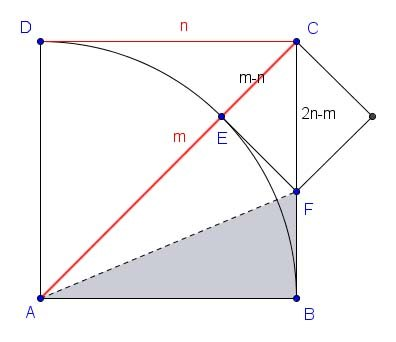
\includegraphics[scale=1.5]{img/irrational}
 \caption{正方形的边长和对角线}
 \label{fig:irrational}
\end{figure}

\begin{proof}
十九世纪的苏格兰数学家乔治·克里斯托尝试重建了古希腊人的证明。使用反证法,假设存在线段$c$能够公度正方形的边和对角线。由度量的定义,令边长为$nc$,对角线长$mc$,其中$m$、$n$都是正整数。如\cref{fig:irrational}所示,以点A为圆心,边长为半径做圆弧交对角线AC于点E。然后从E出发作垂直于对角线的直线,并交边BC于点F。

由圆的定义,线段AE的长度等于正方形的边长,所以线段EC的长度等于$(m - n)c$。因为EF垂直于AC,而角$\angle ECF$是$45\degree$,故三角形ECF是等腰直角三角形。由两腰相等有$|EC| = |EF|$。接下来注意两个直角三角形$\triangle AEF$和$\triangle ABF$,由于边AE等于AB,同时AF是公共边,因此两个直角三角形全等。这样就得到边$|EF| = |FB|$。综合下来,有$|EC| = |EF| = |FB|$。这样线段FB的长度也等于$(m - n)c$,所以线段CF的长度等于CB的长度减去FB的长度,等于$nc - (m - n)c = (2n - m)c$。我们把得到的结论列在下面。

\[
\begin{array}{c|c}
\begin{cases}
|AC| = mc \\
|AB| = nc
\end{cases} &
\begin{cases}
|CF| = (2n - m)c \\
|CE| = (m - n)c
\end{cases} \\[4ex]
\text{大正方形} & \text{小正方形}
\end{array}
\]

由于$m$、$n$都是正整数,$c$也可以公度小正方形的对角线$CF$和边$CE$。仿照上面的方法,我们可以继续作出更小的正方形,并且重复作出无穷无尽的更小的正方形。而$c$总可以公度每一个小正方形的斜边和对角线。由于$m$、$n$是有限的正整数,这一过程不可能无限做下去,这样就产生了矛盾。所以一开始的假设不成立,正方形的边和对角线不可公度。
\end{proof}

类似地,\cref{qn:pentagon-irrational}要求证明正五边形的边长和对角线不可公度。就这样,欧几里得找到了区分有理数和无理数的方法——欧几里得算法是否终止,并由此定义了有理量和无理量。

\index{不可公度}
\begin{proposition}[《原本》,卷十,命题2] \label{th:irrational-gcm}
如果从两个不等量的大量中连续减去小量,直到余量小于小量,再从小量中连续减去余量直到小于余量,这样一直作下去,当所余的量总不能量尽它前面的量时,则称两个量不可公度。
\end{proposition}

\begin{definition}[《原本》,卷十,定义3]
与给定线段可公度的线段是\underdot{有理}线段,凡与此线段不可公度的线段叫做\underdot{无理}线段。
\end{definition}

\subsection{欧几里得算法的应用}

欧几里得算法有着诸多的应用。第\ref{sec:linear-diophantus-equation}节展示了如何使用扩展欧几里得算法给出二元一次丢番图方程$ax + by = c$的整数解。具体来说,就是先求出最大公度$d$,并判断$d$是否整除$c$,若不能,则无整数解。否则,将满足贝祖等式的$x_0$,$y_0$,扩大$c/d$倍得到一组特解$x_1$、$y_1$,然后得到通解$x = x_1 - k b / d$和$y = y_1 + k a / d$。欧几里得算法是最著名的递归算法。德国数学家狄利克雷(Dirichlet)在他的著作《数论讲义》中评价到:“整个数论的结构都建立在同一个基础之上,这个基础就是欧几里得算法。”现代密码学的RSA加密算法\footnote{RSA算法是最早的一种公开密钥加密的非对称加密算法,1977年由罗纳德·李维斯特(Ron Rivest)、阿迪·萨莫尔(Adi Shamir)和伦纳德·阿德曼(Leonard Adleman)一起提出的。当时他们三人都在麻省理工学院工作。RSA就是他们三人姓氏开头字母拼在一起组成的。}直接使用了扩展欧几里得算法。这颗数论的明珠支持了今天的互联网通讯和电子交易。我们接下来再通过两个例子了解欧几里得算法的威力:一个是算术基本定理,另一个是连分数。

\subsubsection{算术基本定理}

\begin{theorem}[算术基本定理]
任何正整数可以表示成素数的积,若不考虑这些素数的顺序,则这种表示是唯一的。
\end{theorem}

例如$12 = 2 \times 2 \times 3 = 2 \times 3 \times 2$,这两种分解只有2, 3的顺序不同,本质上是一种分解$2^2 \times 3$。算术基本定理明确地告诉我们,素数是构成整数的基本砖石,并且这种构造是唯一确定的。为了证明算术基本定理,我们第一步先证明:

\begin{lemma}[欧几里得]
如果素数$p$整除积$ab$,其中$a, b$是互素的数,那么要么$p$整除$a$,要么$p$整除$b$。
\end{lemma}

\begin{proof}
假设$p$不整除$a$,把欧几里得算法应用到$p, a$上,可以得到它们的最大公约数1,然后根据贝祖等式得到:

\begin{align*}
px + ay &= 1 && \text{贝祖等式} \\
pxb + aby & = b && \text{两边乘以}b
\end{align*}

$p$整除左边的第一项,由于$p$整除$ab$,所以$p$也整除左边的第二项。因此$p$整除左边,所以$p$整除$b$。
\end{proof}

有了这个引理,就可以证明算术基本定理了。

\begin{proof}
用反证法,假设某一正整数$n$有两种素数分解:
\[
p_1 p_2 \dotsm p_j = q_1 q_2 \dotsm q_k
\]
其中某个素因子$p_i$不等于右侧任何素因子。根据欧几里得引理,因为素数$p_i$整除彼此互素数的积$n = q_1 q_2 \dotsm q_k$,所以$p_i$要么整除$q_1$,要么整除$q_2$……要么整除$q_k$。但这是不可能的,因为每个素数$q_1, q_2, \dotsc, q_k$都不可能被任何其它素数整除。因此假设不成立,任何正整数$n$只有一种素数分解。
\end{proof}

算术基本定理也被称做唯一分解定理。1843年德国数学家库默尔在研究费马大定理时意识到了唯一分解定理在复整数上可能不成立,这引发了代数数论的诞生(见第6章)。

\subsubsection{连分数}

第二个例子是连分数。如果分子、分母不是整数,而是分数或分数与整数的和,就会构造出更加复杂的分数,例如:$1 + \frac{1}{1 + \frac{1}{2}}$,它的值是$\frac{5}{3}$。这样的构造甚至可以是无限的,例如:

\[
x = 1 + \dfrac{1}{2 + \dfrac{1}{3 + \dfrac{1}{4 + \dfrac{1}{\dotso}}}}
\]

用代数符号表示就是:

\be
x = n_1 + \dfrac{1}{n_2 + \dfrac{1}{n_3 + \dfrac{1}{n_4 + \dfrac{1}{\dotso}}}}
\ee

人们把形如这样的分数叫做连分数,连分数可以是有限的或者无限的。有限的连分数虽然复杂,但是毕竟经过有限步的分数加法、除法可以化简为普通的分数值,例如上面例子中的$\frac{5}{3}$。但无限的连分数有确定的值么?如果有的话,有什么样的规律?我们甚至可以想象一些有趣的模式,例如$1 = n_1 = n_2 = \dotso $,这个连分数形如:

\[
x = 1 + \dfrac{1}{1 + \dfrac{1}{1 + \dfrac{1}{1 + \dfrac{1}{\dotso}}}}
\]

它的值是什么?如果$n_1, n_2, \dotsc$像无限循环小数那样形成循环节时会怎样?如果它们不循环,但是一个无限的序列,如$1, 2, 3, \dotso$时,这个连分数的值会是什么?所有这些有趣问题都令人兴奋。而欧几里得算法给了我们一个对连分数的解读方法。考虑$x = \frac{42}{30}$。

\begin{enumerate}[第1步,]
\item 使用带余数除法:$42 = 30 \times 1 + 12$,所以$x$的整数部分$n_1 = 1$,剩余部分为$\frac{12}{30}$, 放在一起就是$x = 1 + \frac{1}{\frac{30}{12}}$。
\item 对$x' = \frac{30}{12}$使用带余数除法:$30 = 12 \times 2 + 6$,所以$x'$的整数部分$n_2 = 2$,剩余部分为$\frac{6}{12}$,放在一起就是:
\[
x = 1 + \dfrac{1}{2 + \dfrac{1}{\dfrac{12}{6}}}
\]
\item 对$x'' = \frac{12}{6}$使用带余数除法:$12 = 6 \times 2 + 0$,所以$x''$的整数部分$n_3 = 2$,没有剩余部分,所以最终的连分数为:
\[
\dfrac{42}{30} = 1 + \dfrac{1}{2 + \dfrac{1}{2}}
\]
\end{enumerate}

\begin{figure}[htbp]
 \centering
 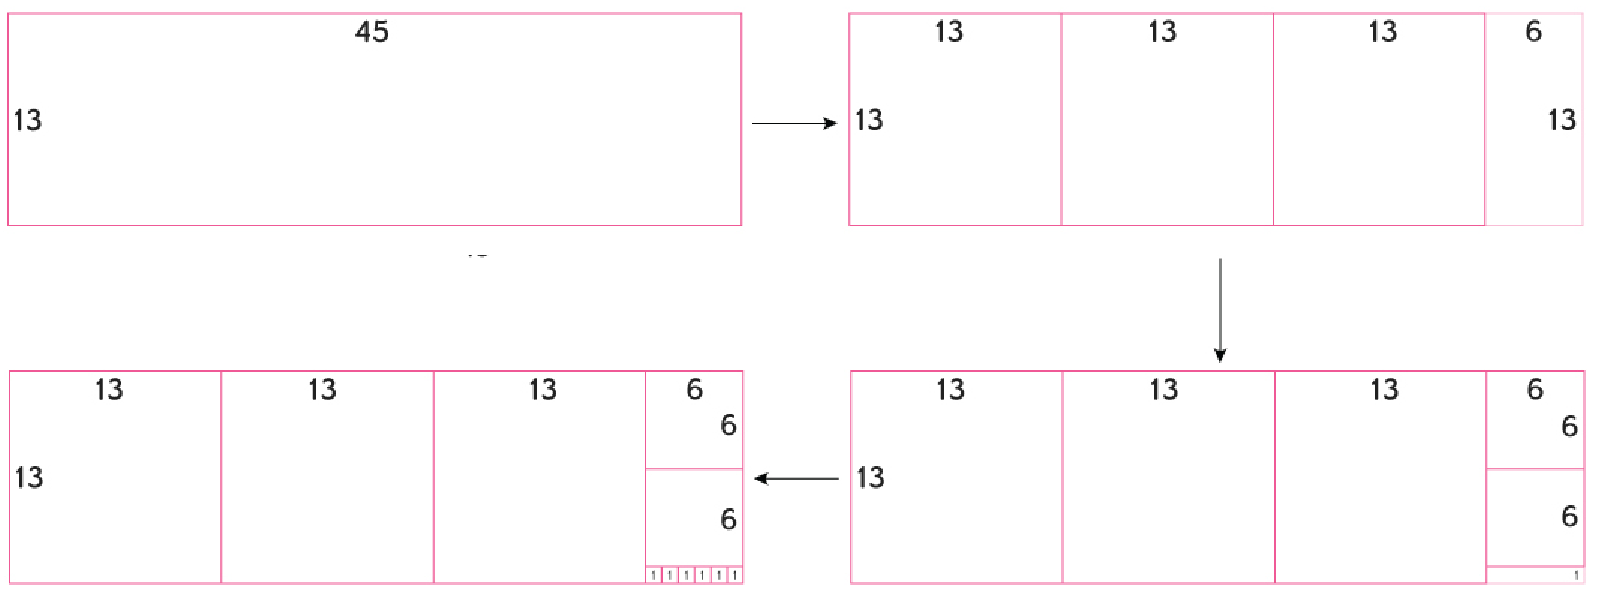
\includegraphics[scale=0.5]{img/cont-frac}
 \caption{用欧几里得算法构造$\dfrac{45}{13} = 3 + \dfrac{1}{2 + \dfrac{1}{6}}$}
 \label{fig:cont-frac}
\end{figure}

这样看来,欧几里得算法就是构造连分数的过程。\cref{fig:cont-frac}给出了用欧几里得算法构造连分数的几何解释。我们根据命题\ref{th:irrational-gcm}知道无理数是不可公度的,欧几里得算法不会停止。一旦把欧几里得算法应用到无理数$x$上,就会构造出无限连分数。让我们用$x = \sqrt{2}$试试看:

\begin{enumerate}[第1步,]
\item 由于$1 < 2 < 4$,开方后有$1 < \sqrt{2} < 2$。所以$x = \sqrt{2}$的整数部分$n_1 = 1$,剩余部分为$x - n_1 = \sqrt{2} - 1$,放在一起就是
\[
 \sqrt{2} = 1 + (\sqrt{2} - 1) = 1 + \dfrac{1}{\dfrac{1}{\sqrt{2} - 1}}
\]
\item 考虑$x' = \dfrac{1}{\sqrt{2} - 1}$,利用平方差公式化简:
  \begin{align*}
    x' = \dfrac{1}{\sqrt{2} - 1} = \dfrac{\sqrt{2} + 1}{(\sqrt{2} - 1)(\sqrt{2} + 1)} = \dfrac{\sqrt{2} + 1}{2 - 1} = \sqrt{2} + 1
  \end{align*}
  由于$1 < \sqrt{2} < 2$,所以$2 < \sqrt{2} + 1 < 3$。因此$x' = \sqrt{2} + 1$的整数部分$n_2 = 2$,剩余部分为$x' - n_2 = \sqrt{2} + 1 - 2 = \sqrt{2} - 1$。这和第一步的剩余部分相同。放在一起就是
\[
 \sqrt{2} = 1 + \dfrac{1}{2 + \dfrac{1}{\sqrt{2} - 1}}
\]
\end{enumerate}
到这里就重复循环了。我们获得了$\sqrt{2}$的无限连分数表示:

\[
 \sqrt{2} = 1 + \dfrac{1}{2 + \dfrac{1}{2 + \dfrac{1}{2 + \dfrac{1}{\dotso}}}}
\]

我们能想象在没有计算机排版前,印刷连分数是多么困难。为此数学家们引入了连分数记法$[n_1; n_2, n_3, \dotso]$。注意第一个分隔符是分号,后面是逗号。使用这个记法,无理数$\sqrt{2} = [1; 2, 2, \dotso]$。并且我们发现$\sqrt{2} + 1 = [2; 2, 2, \dotso]$构成了完美的循环。\cref{qn:phi-continue-frac}要求给出黄金分割数$\phi$的连分数表示。回顾分数和小数的关系:有理数可以表示成有限和无限循环的小数,但无理数只能表示成无限不循环的小数;有理数可以表示成有限的连分数,一些无限不循环的小数却可以表示成无限循环的连分数。那么有没有只能表示成无限不循环连分数的无理数呢?有的,我们熟悉的圆周率$\pi$就是这样的数。让我们继续这段无理数的旅程。

\begin{Exercise}[label={ex:irrationals}]
\Question{正五边形数}
\Question{\cref{fig:garfield}是第20任美国加菲尔德的勾股定理证法,请解释这一证明。\label{qn:pythagoras-thm-garfield}
\begin{center}
 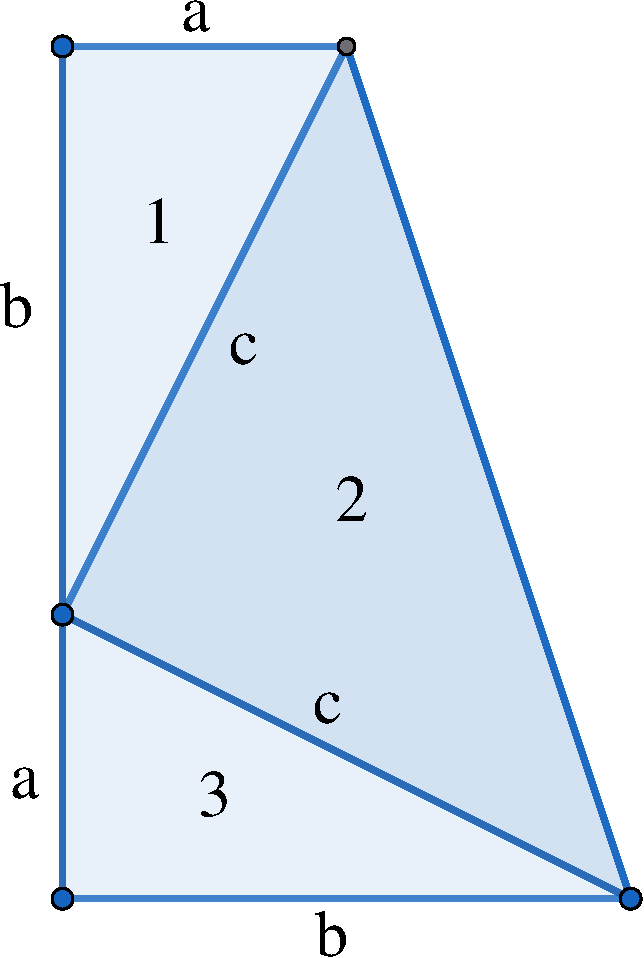
\includegraphics[scale=0.3]{img/garfield}
 \captionof{figure}{美国总统詹姆斯·加菲尔德证法(1876)}
 \label{fig:garfield}
\end{center}
}

\Question{\cref{fig:mosaic}是一家老饭店地面上铺的瓷砖,你能从中看出勾股定理么?
\begin{center}
 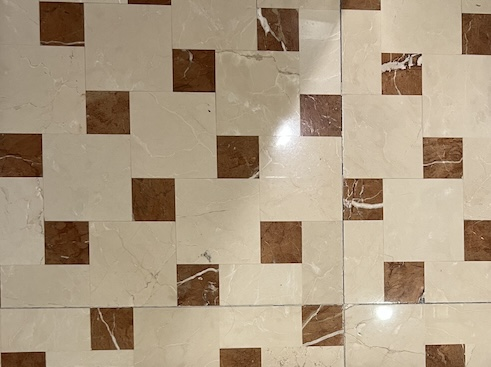
\includegraphics[scale=0.4]{img/mosaic}
 \captionof{figure}{勾股定理与马赛克瓷砖。}
 \label{fig:mosaic}
\end{center}
}

\Question{$a, b$是互素的奇数,证明$\frac{a \pm b}{2}$互素。\label{qn:coprime-of-half-a-pm-b}}

\Question{数论中的\underdot{算术基本定理}说:任何整数可以表示成素数的积,不考虑顺序的情况下,这种表示是唯一的。使用算术基本定理证明:$a, b$互素,若$ab = c^2$,则$a, b$都是平方数。\label{qn:coprime-product-as-square}}

\Question{利用埃拉托斯特尼筛法找出100以内的所有素数。\label{qn:seive-of-eratosthenes-100}}

\Question{任给一条线段$AB$,(1) 作其通过$A$点的垂线。(2) 作通过不在$AB$上的一点$C$的垂线。\label{qn:perp-of-point}}

\Question{给定直线$l$和不在直线上的一点$p$,作通过$p$平行$l$的直线。\label{qn:parallel-through-p}}

\Question{古希腊的圆规抬起后两脚合拢,无法像今天的圆规那样直接截取线段。在古希腊,给定一条线段$AB$和一条直线$l$,如何在$l$上截取长度$AB$?\label{qn:mark-off-segment}}

\Question{我们在证明欧几里得算法正确性的过程中说:“每次都保证余数小于除数。即$b > r_0 > r_1 > r_2 > ... > 0$,但是余数不可能小于零。由于起始值是有限的,故最终算法一定中止。”为什么不会出现,$r_{n}$无限接近于零但不等于零的情况?算法一定会中止么?$a$和$b$是可公度的这一前提保证了什么?}

\Question{对于二元线性不定方程$ax + by = c$,若$x_1$、$y_1$和$x_2$、$y_2$为两对整数解。试证明$|x_1 - x_2|$的最小值为$b/(a, b)$,且$|y_1 - y_2|$的最小值为$a/(a, b)$。}

\Question{找出用9升和4升的瓶子从河中打出6升水的最少步骤。\label{qn:best-steps-water}}

\Question{证明正五边形的边长和对角线不可公度。\label{qn:pentagon-irrational}}

\Question{黄金分割数$\phi = \frac{1 + \sqrt{5}}{2}$的连分数表示是什么?\label{qn:phi-continue-frac}}

\end{Exercise}

%% ========== 答案 ====================

\begin{Answer}[ref={ex:irrationals}]
\Question{正五边形数}

\Question{梯形面积等于两个原直角三角形和一个等腰直角三角形的面积和
}

\Question{%\cref{fig:mosaic}是一家老饭店地面上铺的瓷砖,你能从中看出勾股定理么?
见\cref{fig:pythagoras-mosaic}中的辅助线。
\begin{center}
 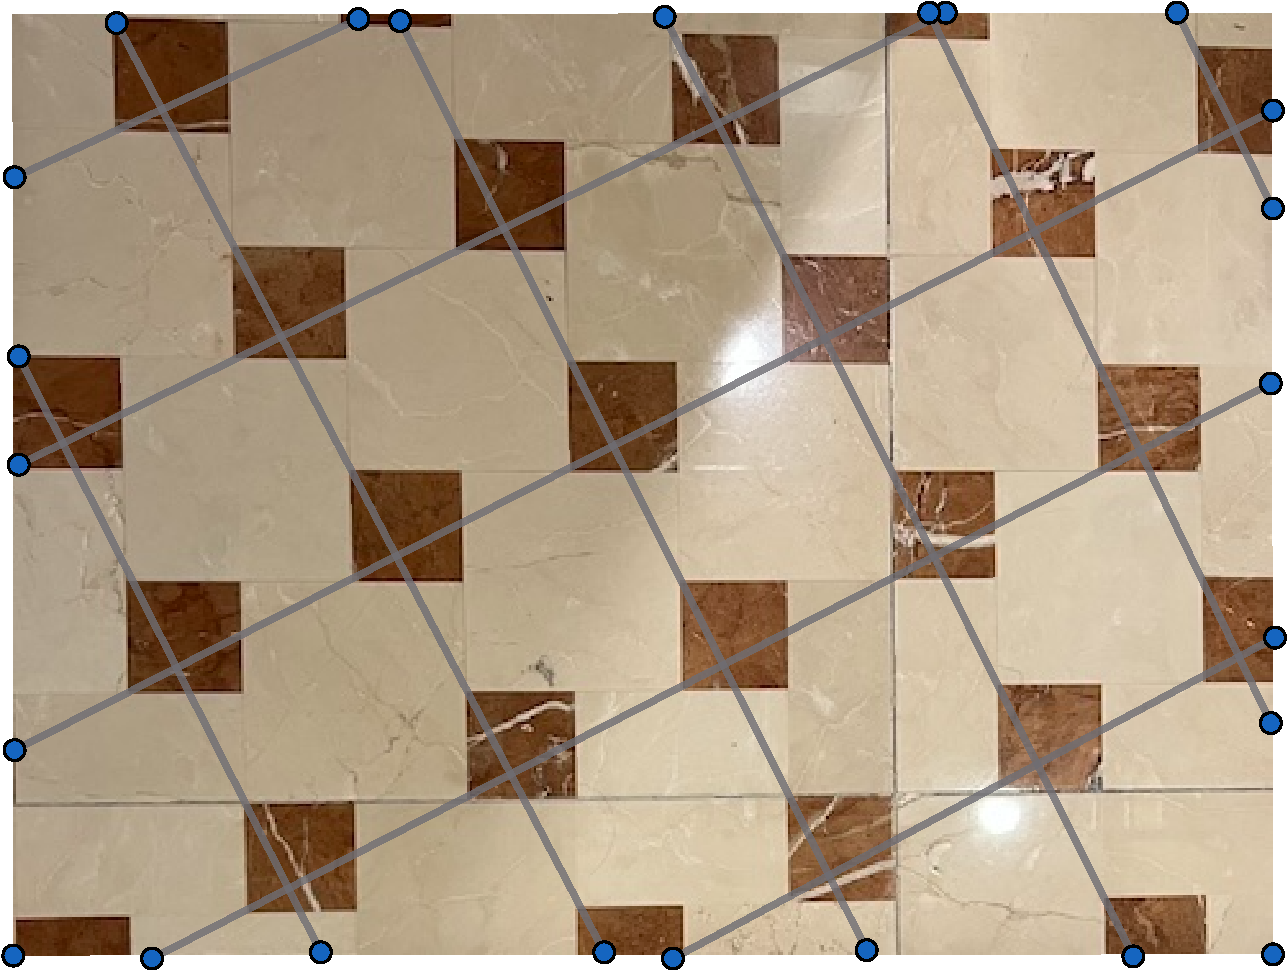
\includegraphics[scale=0.4]{img/pythagoras-mosaic}
 \captionof{figure}{勾股定理与马赛克瓷砖。}
 \label{fig:pythagoras-mosaic}
\end{center}
}

\Question{%%$a, b$是互素的奇数,证明$\frac{a \pm b}{2}$互素。
  \begin{proof}
    设$d$为$\frac{a \pm b}{2}$的公因子,令$dm = \frac{a + b}{2}, dn = \frac{a - b}{2}$,其中$m, n$为整数。两式相加求得$a = dm + dn = d(m + n)$,所以$d$整除$a$;两式相减得$b = dm - dn = d (m - n)$,所以$d$也整除$b$。这样$d$也是$a, b$的公因子。但$a, b$互素,所以$d$只能是1,即$\frac{a \pm b}{2}$互素。
  \end{proof}
}
\Question{%%$a, b$互素,若$ab = c^2$证明$a, b$都是平方数。
  \begin{proof}
    利用算术基本定理,把$a, b$各自表示为素数幂的积:$a = p_1^{a_1} p_2^{a_2} \dotsm p_n^{a_n}, b = q_1^{b_1} q_2^{b_2} \dotsm q_m^{b_m}$,其中$p_i, q_j$都是素数。由于$a, b$互素,它们的公因数只有1,故$p_i \ne q_j$。它们的积是个平方数$c^2 = p_1^{a_1} p_2^{a_2} \dotsm p_n^{a_n} q_1^{b_1} q_2^{b_2} \dotsm q_m^{b_m}$,所以必然有$a_i, b_j$全部是偶数,即$a, b$都是平方数。
  \end{proof}
}

\Question{利用埃拉托斯特尼筛法找出100以内的所有素数。
}


\Question{任给一条线段$AB$,(1) 作其通过$A$点的垂线。(2) 作通过不在$AB$上的一点$C$的垂线。

如\cref{fig:perp-of-point}所示,反向延长$AB$,以$A$为圆心$AB$为半径交延长线于点$B'$。分别以点$B$和$B'$为圆心,$BB'$为半径画两圆。连接两圆交点得垂线$CD$。
\begin{center}
 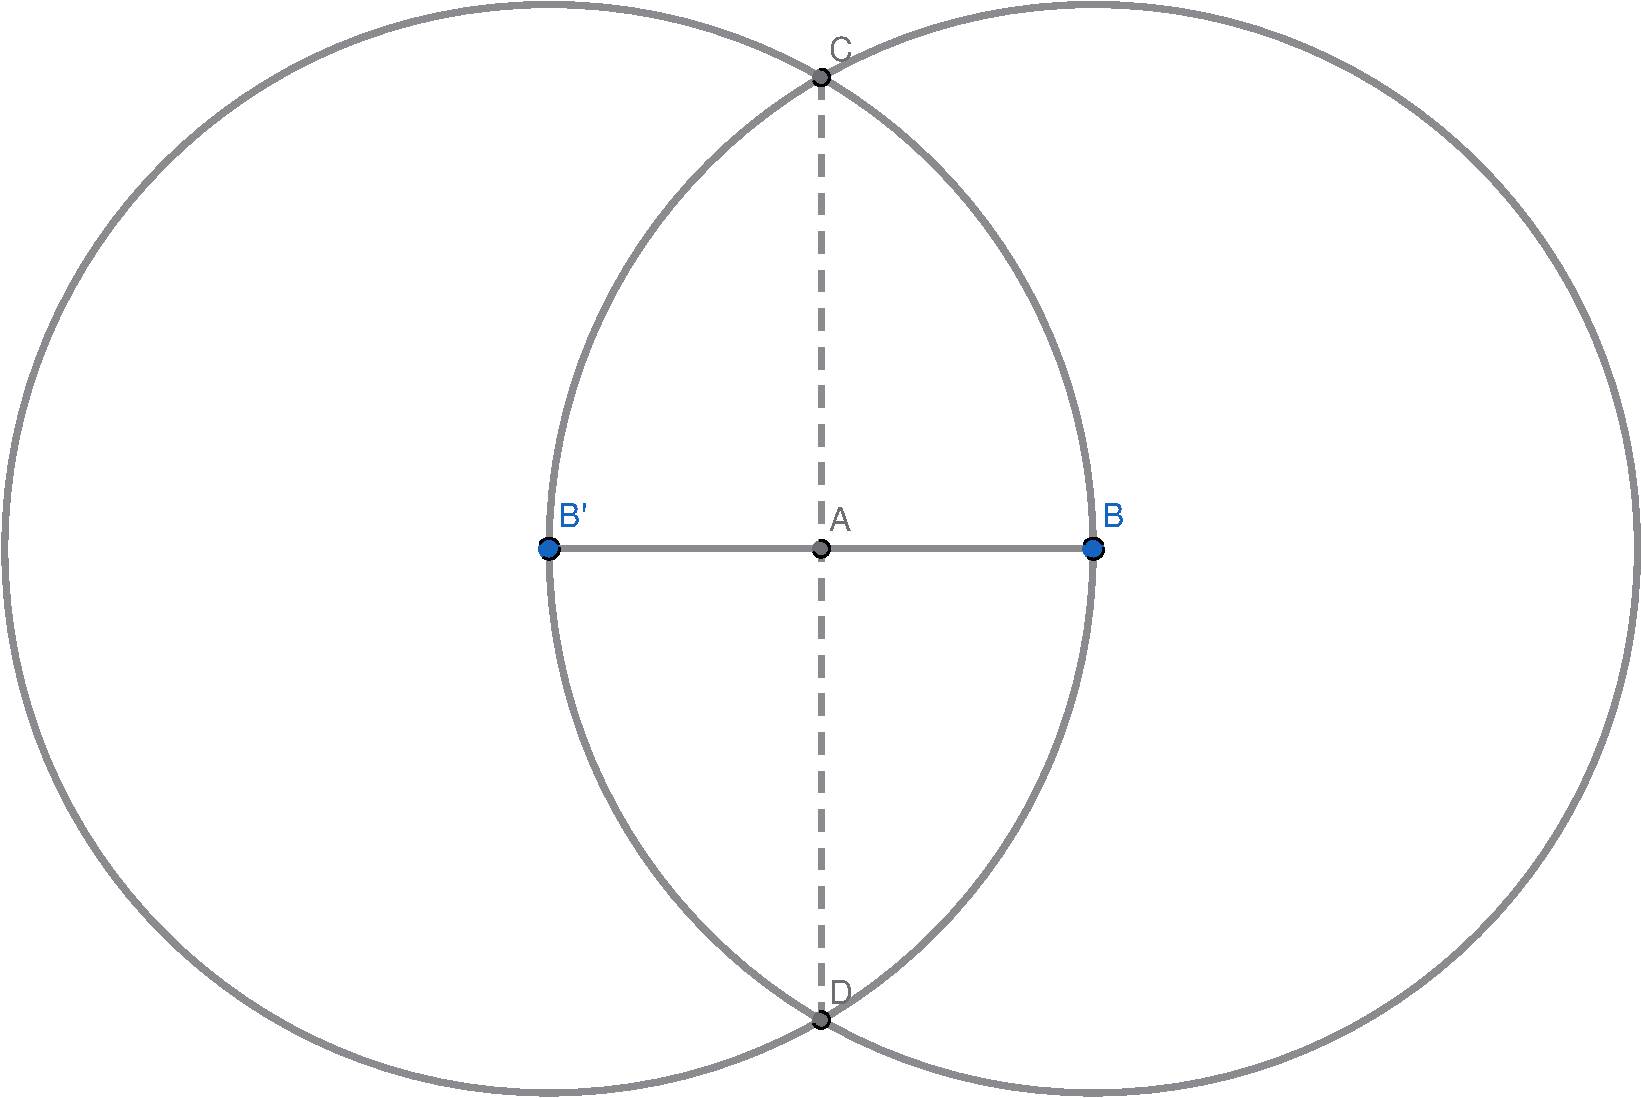
\includegraphics[scale=0.3]{img/perp}
 \captionof{figure}{作过定点的垂线}
 \label{fig:perp-of-point}
\end{center}
}

\Question{给定直线$l$和不在直线上的一点$p$,作通过$p$平行$l$的直线。}

\Question{古希腊的圆规抬起后两脚合拢,无法像今天的圆规那样直接截取线段。在古希腊,给定一条线段$AB$和一条直线$l$,如何在$l$上截取长度$AB$?}

\Question{%%我们在证明欧几里得算法正确性的过程中说:“每次都保证余数小于除数。即$b > r_0 > r_1 > r_2 > ... > 0$,但是余数不可能小于零。由于起始值是有限的,故最终算法一定中止。”为什么不会出现,$r_{n}$无限接近于零但不等于零的情况?算法一定会中止么?$a$和$b$是可公度的这一前提保证了什么?

\begin{proof}
由$a, b$可公度,令$a = nc, b = mc$。由带余数除法$a = bq + r_0$,有$r_0 = a - bq = (n - mq)c$,也可被$c$度量。以此类推$b > r_0 > r_1 > \dotsb \geq 0$都可被$c$度量。用$c$除以每个值得到一系列递减的\underdot{整数}:$m > n - mq > \dotsb \geq 0$。而$m$是有限的整数,因此这个序列必然有限,而不会无限接近但不等于0。
\end{proof}
}

\Question{%%对于二元线性不定方程$ax + by = c$,若$x_1$、$y_1$和$x_2$、$y_2$为两对整数解。试证明$|x_1 - x_2|$的最小值为$b/(a, b)$,且$|y_1 - y_2|$的最小值为$a/(a, b)$。

令$a, b$的最大公约数$d = (a, b)$。如果$x_0, y_0$是不定方程$ax + by = c$的一组解,则下面给出的也是一组解:

\[
\begin{dcases}
  x = x_0 - k \dfrac{b}{d} \\
  y = y_0 + k \dfrac{a}{d}
\end{dcases}
\]

这一点不难证明:

\blre
ax + by & = & a (x_0 - k \dfrac{b}{g}) + b (y_0 - k \dfrac{a}{d}) \\
        & = & a x_0 + b y_0 - a k \dfrac{b}{g} + b k \dfrac{a}{d} \\
        & = & c - 0 = c
\elre

我们接下来证明,所有不定方程的解都可以表示为这一形式。令$x, y$为不定方程的任意一组解,我们有:$ax + by = c$和$a x_0 + b y_0 = c$。因此:

\[
a (x - x_0) + b (y - y_0) = c - c = 0
\]

两边同时除以$a, b$的最大公约数,得:

\[
\dfrac{a}{d} (x - x_0) + \dfrac{b}{d} (y - y_0) = 0
\]

\[
\dfrac{b}{d} (y - y_0)  = - \dfrac{a}{d} (x - x_0)
\]

注意到,左侧能够被$\dfrac{b}{d}$整除,因此它必然也能整除右侧。但是由于$(\dfrac{a}{d}, \dfrac{b}{d}) = 1$,它们互素,所以必然有$\dfrac{b}{d}$整除$(x - x_0)$,不妨令:

\[
x - x_0 = k \dfrac{b}{d}, \text{对于某个} k \in \pmb{Z}
\]

因此

\[
x = x_0 + k \dfrac{b}{d}
\]

将其代入回上面的等式,得出:

\[
y = y_0 - k \dfrac{a}{d}
\]

这样就证明了所有解都必然是这样的形式。显然,任意两组这样的解,其差最小时$k = 1$,即:$|x_1 - x_2|$的最小值为$b/(a, b)$,且$|y_1 - y_2|$的最小值为$a/(a, b)$。
}

\Question{找出用9升和4升的瓶子从河中打出6升水的最少步骤。
}

\Question{%%证明真五边形的边长和对角线不可公度。

\begin{proof}
用反证法,假设它们是可公度的。令边长为$mc$,对角线为$nc$,其中$m, n$是整数。如\cref{fig:pentagon-irrational}所示,由BEC是等腰三角形,所以$EC = BE = nc$;由ABE和FBE全等,$AB = FE = mc$。所以$FC = EC - FE = (n-m)c$。因此小五边形的对角线$CD = mc$和边长$FC = (n -m)c$也是可公度的。我们可以无限重复这个过程,获得越来越小的五边形而不终止。这与$m, n$是有限的正整数矛盾。因此假设不成立,正五边形的边长和对角线不可公度。
\end{proof}

\begin{center}
  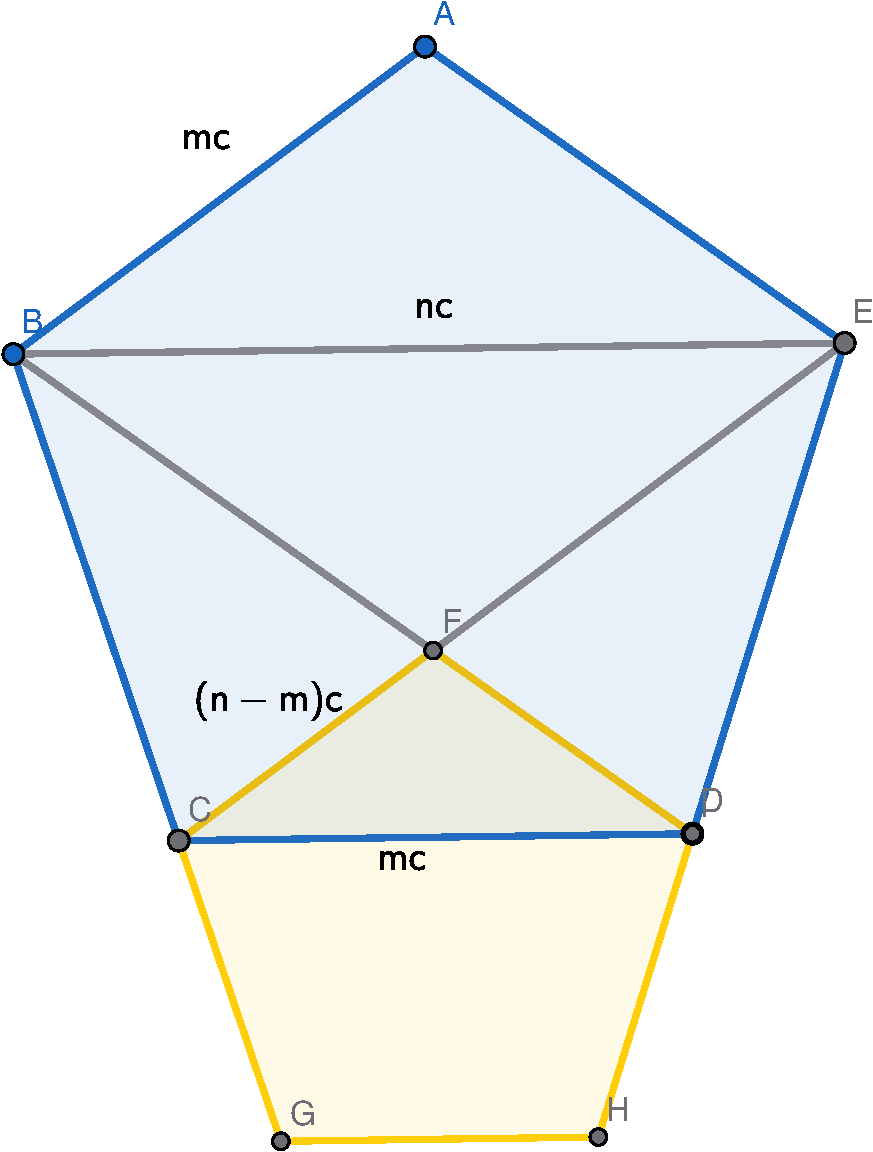
\includegraphics[scale=0.3]{img/pentagon-irr}
  \captionof{figure}{正五边形的边与对角线}
  \label{fig:pentagon-irrational}
\end{center}
}

\Question{%黄金分割数$\phi = \frac{1 + \sqrt{5}}{2}$的连分数表示是什么?

由$\phi \approx 1.618$,故$\phi$的整数部分$n_1 = 1$,剩余部分$\frac{1 + \sqrt{5}}{2} - 1 = \frac{\sqrt{5} - 1}{2}$,即:
\begin{align*}
  \phi &= 1 + \dfrac{\sqrt{5} - 1}{2} = 1 + \dfrac{1}{\dfrac{1}{\dfrac{\sqrt{5} - 1}{2}}}  \\
  &= 1 + \dfrac{1}{\dfrac{\sqrt{5} + 1}{2}} && \dfrac{\sqrt{5} \pm 1}{2} \text{互为倒数} \\
  &= 1 + \dfrac{1}{\phi} = 1 + \dfrac{1}{1 + \dfrac{1}{\phi}} \\
  &= 1 + \dfrac{1}{1 + \dfrac{1}{1 + \dfrac{1}{\dotso}}}
\end{align*}
故黄金分割数的连分数表示是$\phi = [1; 1, 1, \dotso]$也是一个完美的循环。
}

\end{Answer}

\chapter{实数}

\epigraph{山巅一寺一壶酒}{圆周率的谐音口诀}

古希腊人通过尺规作图构造出了用加减乘除四则运算无法产生的数——无理数。从运算的角度思考,尺规作图究竟代表了什么特殊的运算?反过来从作图的角度思考,四则运算能否都能用尺规作图实现?通过探索这两个互逆的问题能否发现更多的无理数?

\section{尺规作图与运算}
\label{sec:geometric-arthimetic}
在求线段最大公度的欧几里得算法中,需要在线段$a$上截掉指定长度$b$,这对应着减法运算$a - b$。反过来,把线段$a$延长,然后在延长线上截取$b$对应着加法运算$a + b$(见\cref{qn:mark-off-segment})。如何实现乘法$ab$呢?有读者说画一个长$a$宽$b$的矩形,面积就是$ab$了。但是古希腊人思考的是如何作出一条线段,其长度是$ab$。他们从欧几里得几何中找到了工具——相似三角形。

\begin{figure}[htbp]
 \centering
 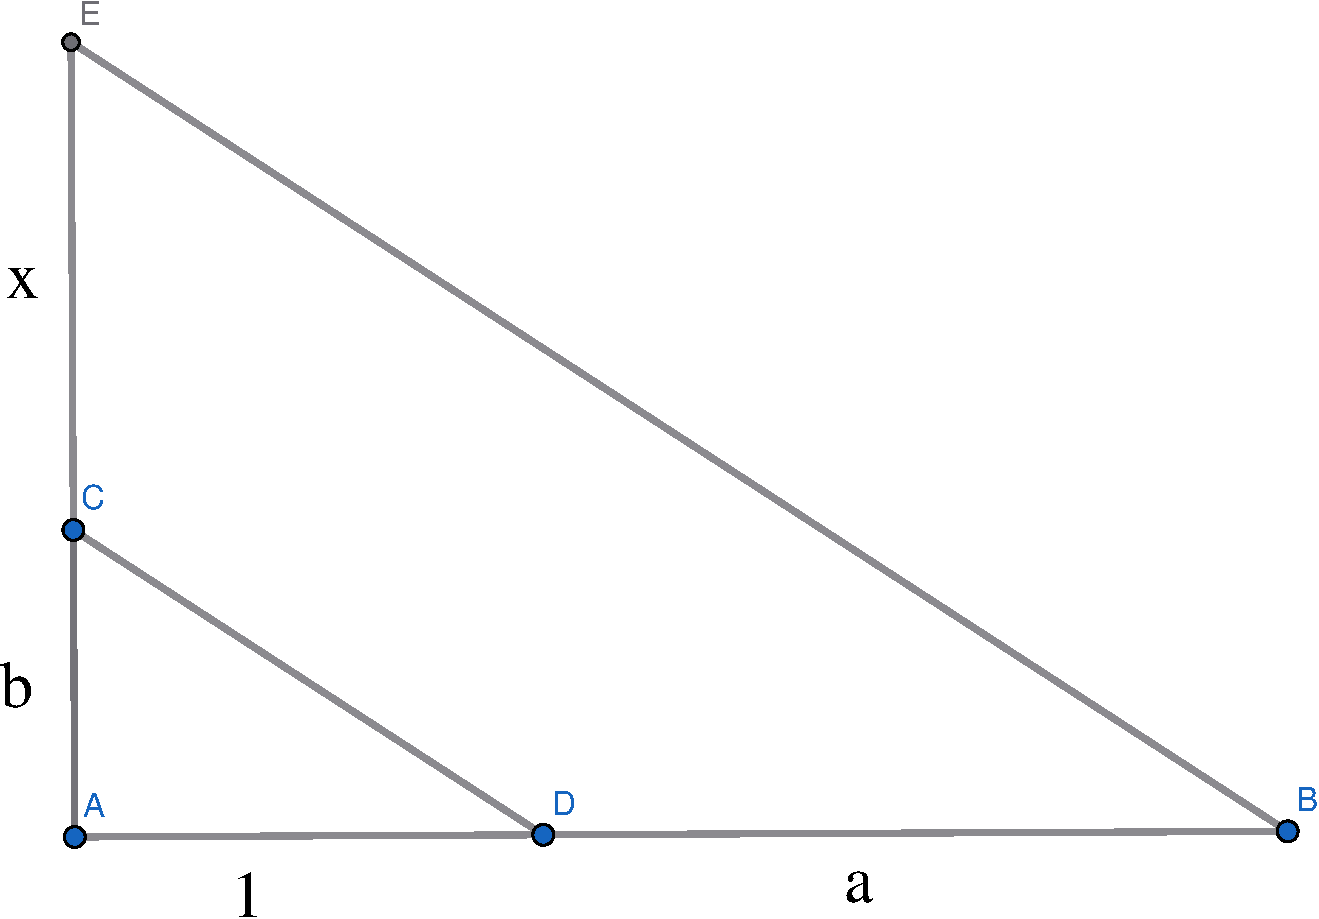
\includegraphics[scale=0.35]{img/product}
 \caption{尺规作图和乘法运算}
 \label{fig:product}
\end{figure}

\begin{proposition}
给定单位线段(长度为1的线段),线段$a$和$b$,可以作出长为$ab$的线段。
\end{proposition}

\begin{proof}
如\cref{fig:product}所示,在长为1的单位线段AD的一端作垂线并截出长为$b$的线段AC(见\cref{qn:perp-of-point}),在单位线段的延长线上截取长为$a$的线段BD。连接CD构成小三角形ACD。过点B作CD的平行线(见\cref{qn:parallel-through-p})交AC的延长线于点E,从而构成大三角形AEB。由于小三角形ACD和大三角形AEB相似(请读者朋友思考为什么?),所以:

\begin{align*}
\dfrac{1}{b} & = \dfrac{AD}{AC} = \dfrac{AB}{AE} = \dfrac{1 + a}{b + x} && \text{三角形相似} \\
b + x & = b(1 + a) && \text{交叉相乘} \\
x & = b(1 + a) - b = ab && \text{线段CE长为}ab \qedhere
\end{align*}
\end{proof}

这样就建立了尺规作图和乘法运算的对应关系。接下来要解决的是用尺规作图实现除法运算。我们的策略是先用尺规作图实现$a \ne 0$的倒数$\dfrac{1}{a}$,然后再利用乘法运算实现$\frac{b}{a} = b \times \dfrac{1}{a}$。再次利用相似三角形。

\begin{proposition}
给定长为1的单位线段和不等于0的线段$a$,可以作出长度为$\dfrac{1}{a}$的线段。
\end{proposition}

\begin{figure}[htbp]
 \centering
 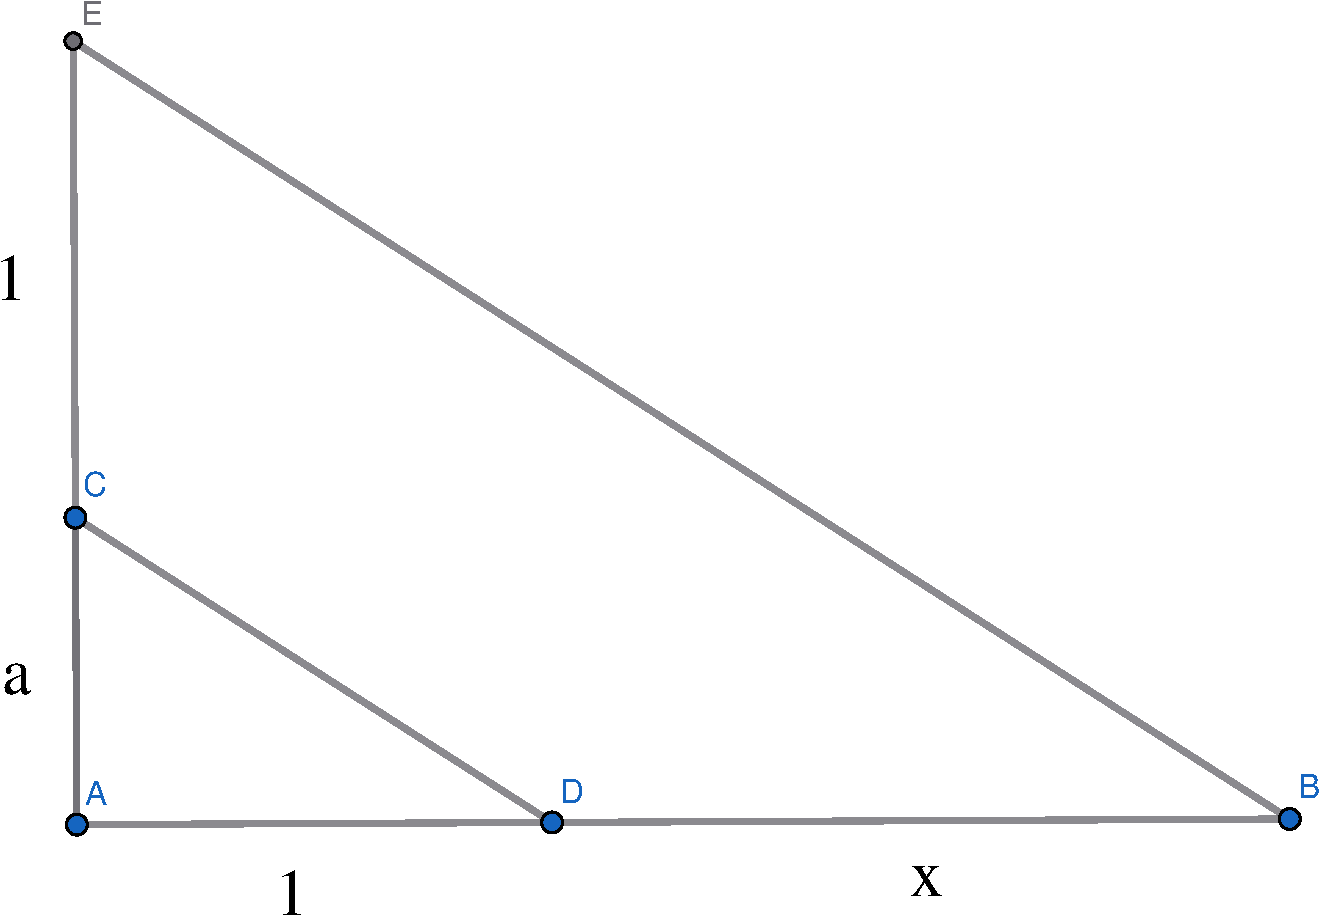
\includegraphics[scale=0.35]{img/reciprocal}
 \caption{尺规作图和倒数运算}
 \label{fig:reciprocal}
\end{figure}

\begin{proof}
如\cref{fig:reciprocal}所示,在长度为1的单位线段AD的一端作垂线并截取长为$a$的线段AC。延长AC并截取长度为1的线段CE。连接CD构成小三角形ACD。过E作平行于CD的直线交AD的延长线于点B。连接BD构成大三角形AEB。由于小三角形ACD和大三角形AEB相似(请读者朋友思考并确认):

\begin{align*}
\frac{1}{a} &= \frac{AD}{AC} = \frac{AB}{AE} = \frac{1 + x}{1 + a}  && \text{三角形相似} \\
a(1 + x) & = 1 + a && \text{交叉相乘} \\
x &= \frac{1 + a}{a} - 1 = \frac{1}{a} && \text{线段BD长为}\frac{1}{a} \qedhere
\end{align*}
\end{proof}

这样就用尺规作图实现了倒数,进而可以实现除法。我们看到加减乘除四则运算都可以由尺规作图实现。由毕达哥拉斯定理,给定长度$a$和$b$的线段,可以作长为$\sqrt{a^2 + b^2}$的线段。接下来我们用尺规作图\underdot{直接}作长为$\sqrt{a}$的线段。

\begin{proposition}\label{thm:sqrt-a}
给定长为1的单位线段和长为$a$的线段,可以作长为$\sqrt{a}$的线段。
\end{proposition}

\begin{figure}[htbp]
 \centering
 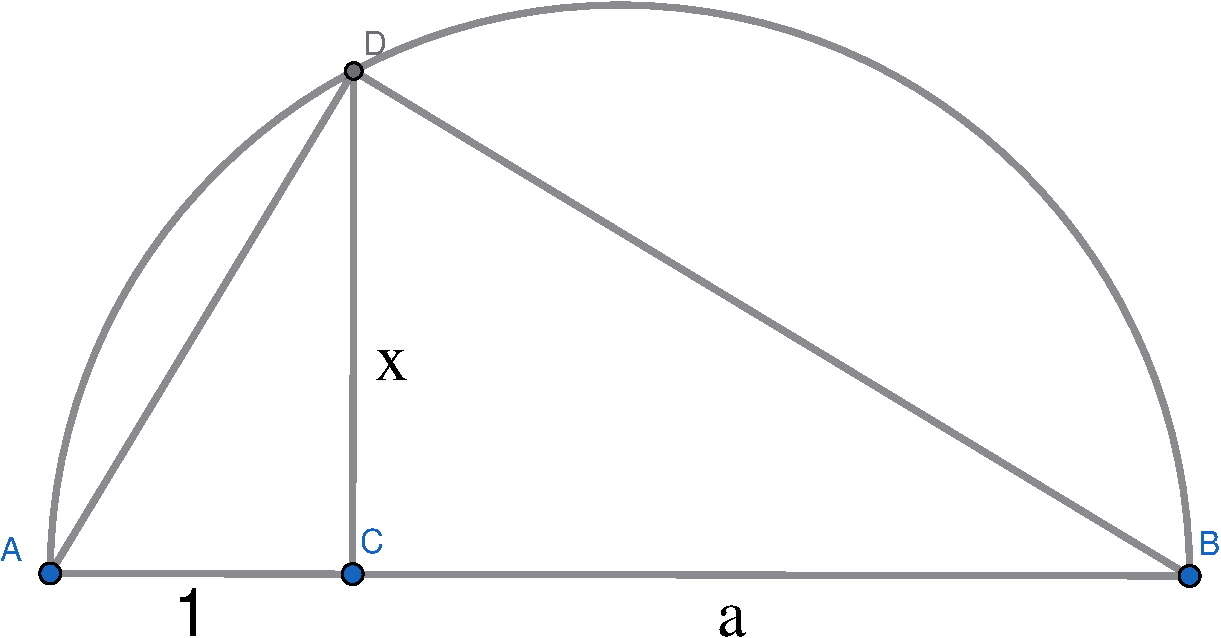
\includegraphics[scale=0.35]{img/sqrt}
 \caption{尺规作图和开方运算}
 \label{fig:sqrt}
\end{figure}

\begin{proof}
如\cref{fig:sqrt}所示,在长度为1的单位线段AC的延长线上截取长度为$a$的线段CB。以AB为直径作圆(作AB的中垂线,以垂足为圆心,垂足到点A的距离为半径)。过C作垂线交圆于点D。连接AD和BD构成小直角三角形ACD和大直角三角形DCB,这两个直角三角形相似(请读者朋友思考并确认)。

\begin{align*}
\frac{1}{x} &= \frac{AC}{CD} = \frac{CD}{CB} = \frac{x}{a} && \text{三角形相似} \\
x^2 &= a && \text{交叉相乘} \\
x &= \sqrt{a} && \text{线段CD长为}\sqrt{a} \qedhere
\end{align*}
\end{proof}

这样我们在义务教育阶段学习过的四则运算和开二次方根运算就都有了各自对应的尺规作图实现。这意味着任何算术运算和开二次方根运算能产生的数都可以通过尺规作图作出。这个结果和毕达哥拉斯学派的想法相反:几何不但没有建立在算术之上,反而算术可以建立在几何之上。古希腊学者并没有停止于此,而是继续探索用尺规作图解决更多的问题。

\subsection{正多边形}

利用尺规古希腊人作出了一系列正多边形,这些正多边形的边长大多是无理数。最简单的正多边形是正三角形。如\cref{fig:polygon}所示,给定一条线段AB,以其为半径,分别以A和B为圆心作圆弧交于点C,连接ABC就获得了正三角形。正四边形就是正方形。作一个圆并作出互相垂直的两条直径。把它们和圆的4个交点连接起来就获得了正方形。如果圆的半径为1,根据勾股定理知正四边形的边长为$\sqrt{2}$。如果能作出正$n$边形,就可以作出正$2n$边形。方法是作每条边的中垂线,这些中垂线交于一点,就是外接圆的圆心。每条中垂线交外接圆周于一点,把这些点和原正$n$变形的定点依次连接起来就获得了正$2n$边形。例如\cref{fig:polygon}中的正六边形就是由正三角形获得的。

\begin{figure}[htbp]
 \centering
 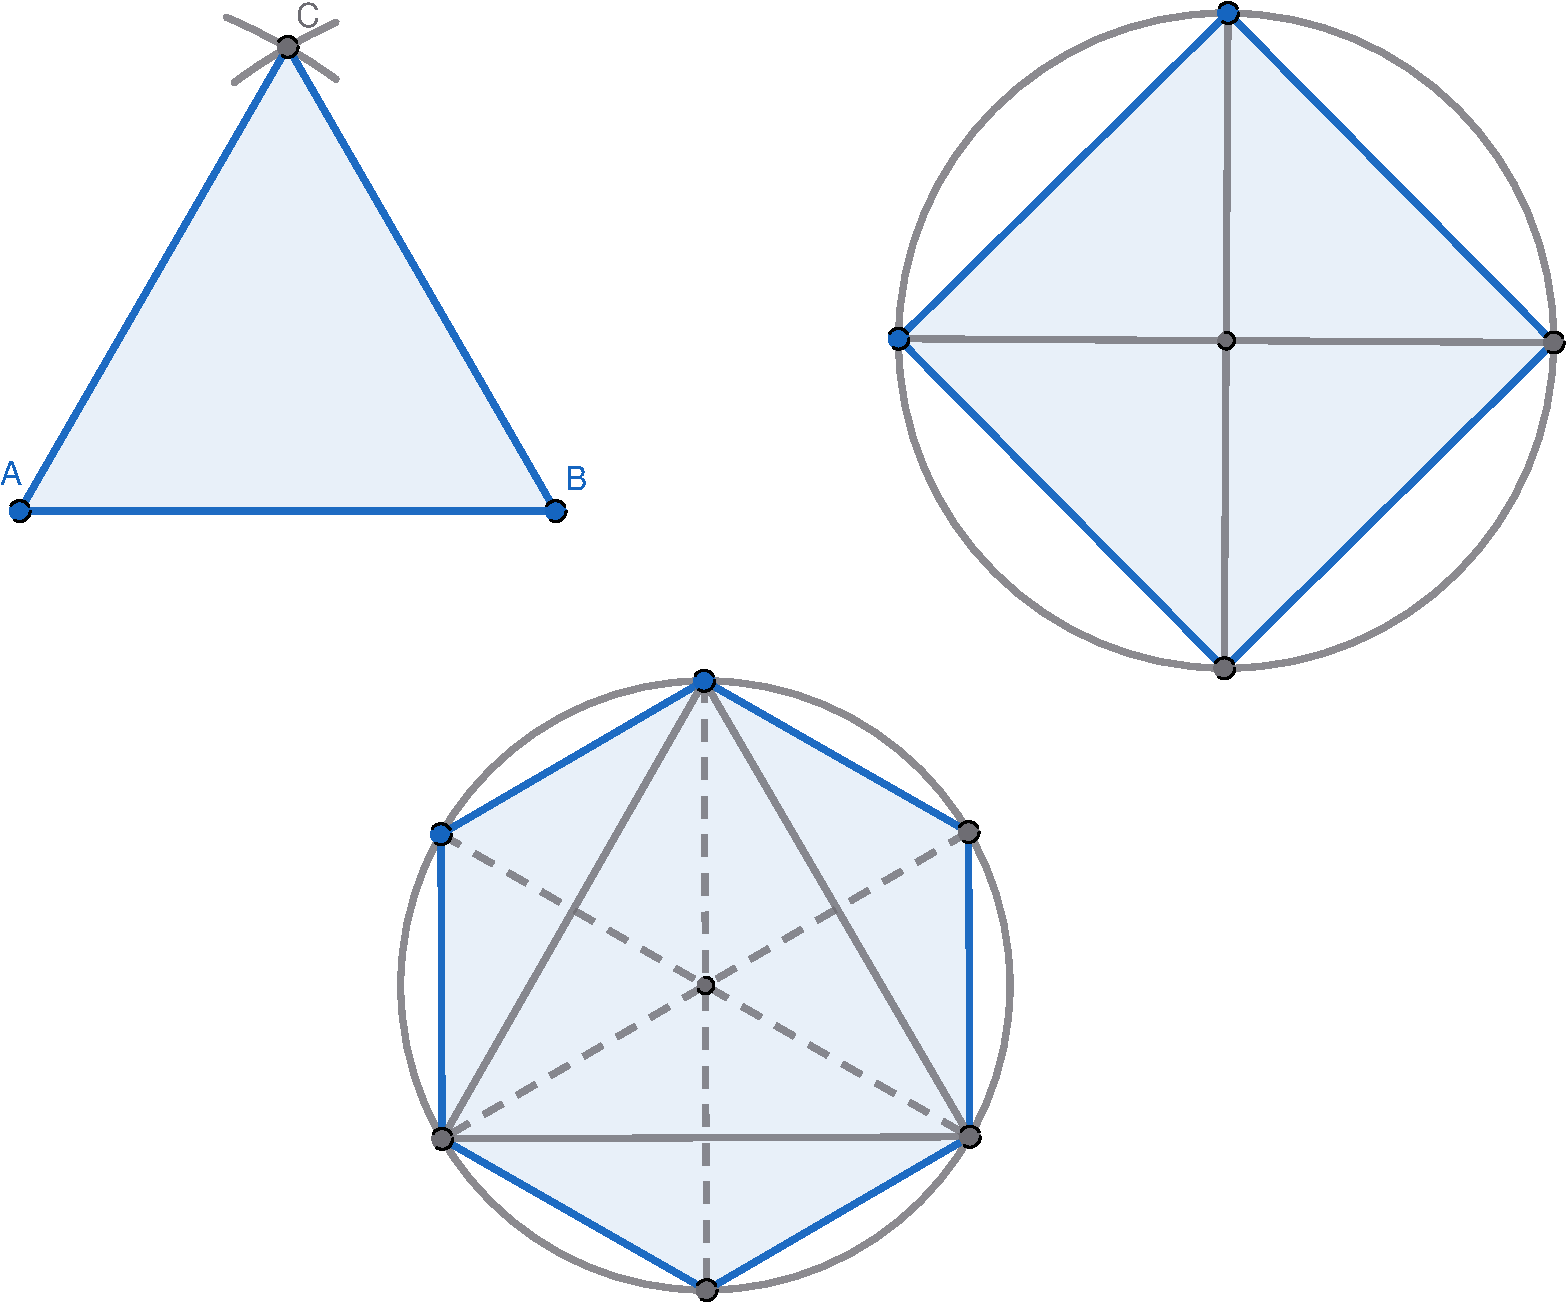
\includegraphics[scale=0.35]{img/polygon}
 \caption{正三角形、正方形、正六边形}
 \label{fig:polygon}
\end{figure}

连接正六边形外接圆的圆心和每个顶点把它划分成6个小正三角形。由此知道如果外接圆半径为1,则正六边形的边长等于1。而其内接正三角形的每个边和两条长为1的半径构成了一个等腰三角形,顶角为120\degree。由此可以计算出正三角形的边长为$\sqrt{3}$。从正四边形可以获得正八边形,我们把边长计算留作练习。作正五边形有一定的难度,但也没有难住古希腊人。我们这里给出两种不同的作图方法。

由第\ref{sec:pentagon-edge}节知,正五边形的对角线为1时,其边长为黄金数$\phi = \dfrac{\sqrt{5}-1}{2}$。这样问题就转变为:如何用尺规做出长度为$\phi$ 的线段?在用毕达哥拉斯(勾股)定理探索无理数时,我们发现$5 = 2^2 + 1^2$。所以任给一条线段,只要做出其2倍长的垂线段,就可构成一直角三角形,根据毕达哥拉斯定理,此三角形的斜边长为$\sqrt{2^2 + 1^2} = \sqrt{5}$。如果将此三角形各边缩小一半,则斜边长为$\dfrac{\sqrt{5}}{2}$,然后在从斜边截去短直角边(长$\dfrac{1}{2}$)就获得了长为$\dfrac{\sqrt{5}-1}{2}$的线段。

\begin{figure}[htbp]
 \centering
 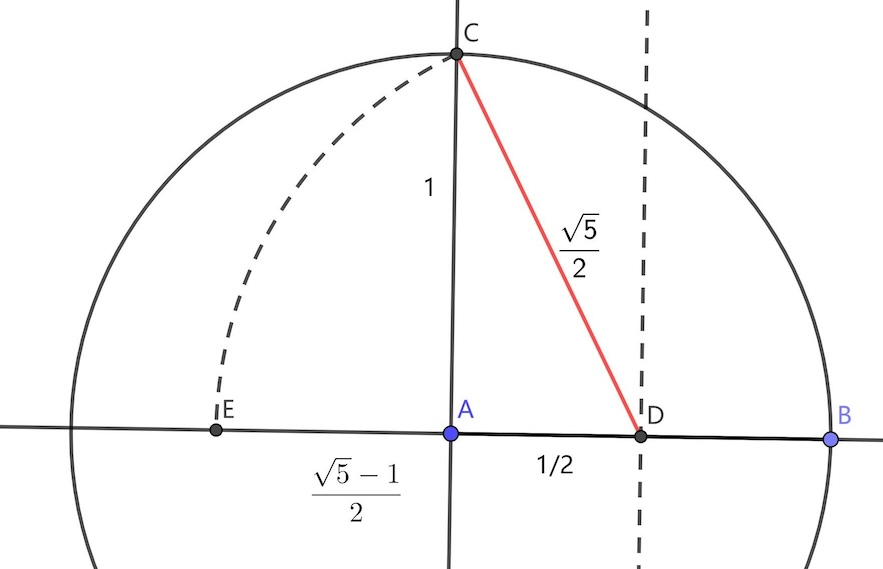
\includegraphics[scale=0.3]{img/phi}
 \caption{作长为$\phi = \dfrac{\sqrt{5} - 1}{2}$的线段}
 \label{fig:phi}
\end{figure}

如\cref{fig:phi}所示,先做单位圆和两条垂直的直径。然后做半径AB的中垂线,这样直角三角形ACD的斜边就是$\dfrac{\sqrt{5}}{2}$。以D为圆心,DC为半径划弧交BA方向的直径于E,则AE长就是$\dfrac{\sqrt{5} - 1}{2}$。

\begin{figure}[htbp]
 \centering
 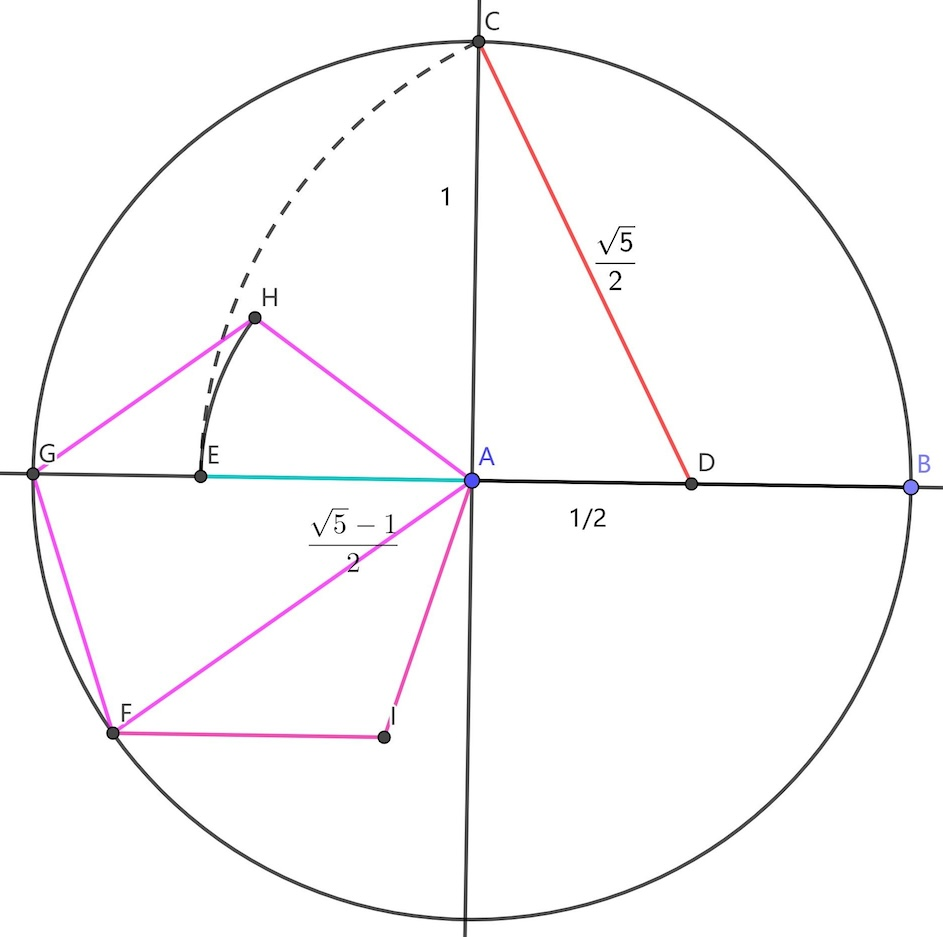
\includegraphics[scale=0.35]{img/pentagon-phi}
 \caption{由线段AE和长为1的半径,做出三个等腰三角形,拼成正五边形。}
 \label{fig:pentagon-phi}
\end{figure}

接下来用长为1和$\phi$的线段可做出\cref{fig:pentagon-phi}中的等腰三角形AHG(边长为1、$\phi$、$\phi$,先作出等腰三角形的底,以底的两个端点为圆心,腰为半径作弧;两弧交于等腰三角形的顶点;最后连接顶点和底的两个端点。)、等腰三角形BEA(边长为1、1、$\phi$)、等腰三角形AIF(边长为1、$\phi$、$\phi$),从而做出正五边形。

第二种正五边形的作法来自欧几里得。他的想法是连接正五边形的中心(即外接圆心)和5个顶点,就会把$360\degree$角均分成5份,每个角是$360 \div 5 = 72\degree$,所以只要想办法作出$72\degree$角问题就突破了。为此欧几里得设计如\cref{fig:isosceles72}所示的等腰三角形。它的底角为顶角的2倍。根据三角形内角和等于$180\degree$可知:$\alpha + 2(2\alpha) = 180\degree$,所以顶角的大小是$180\degree$的$\frac{1}{5}$,即$36\degree$,而底角是$72\degree$。

\begin{figure}[htbp]
 \centering
 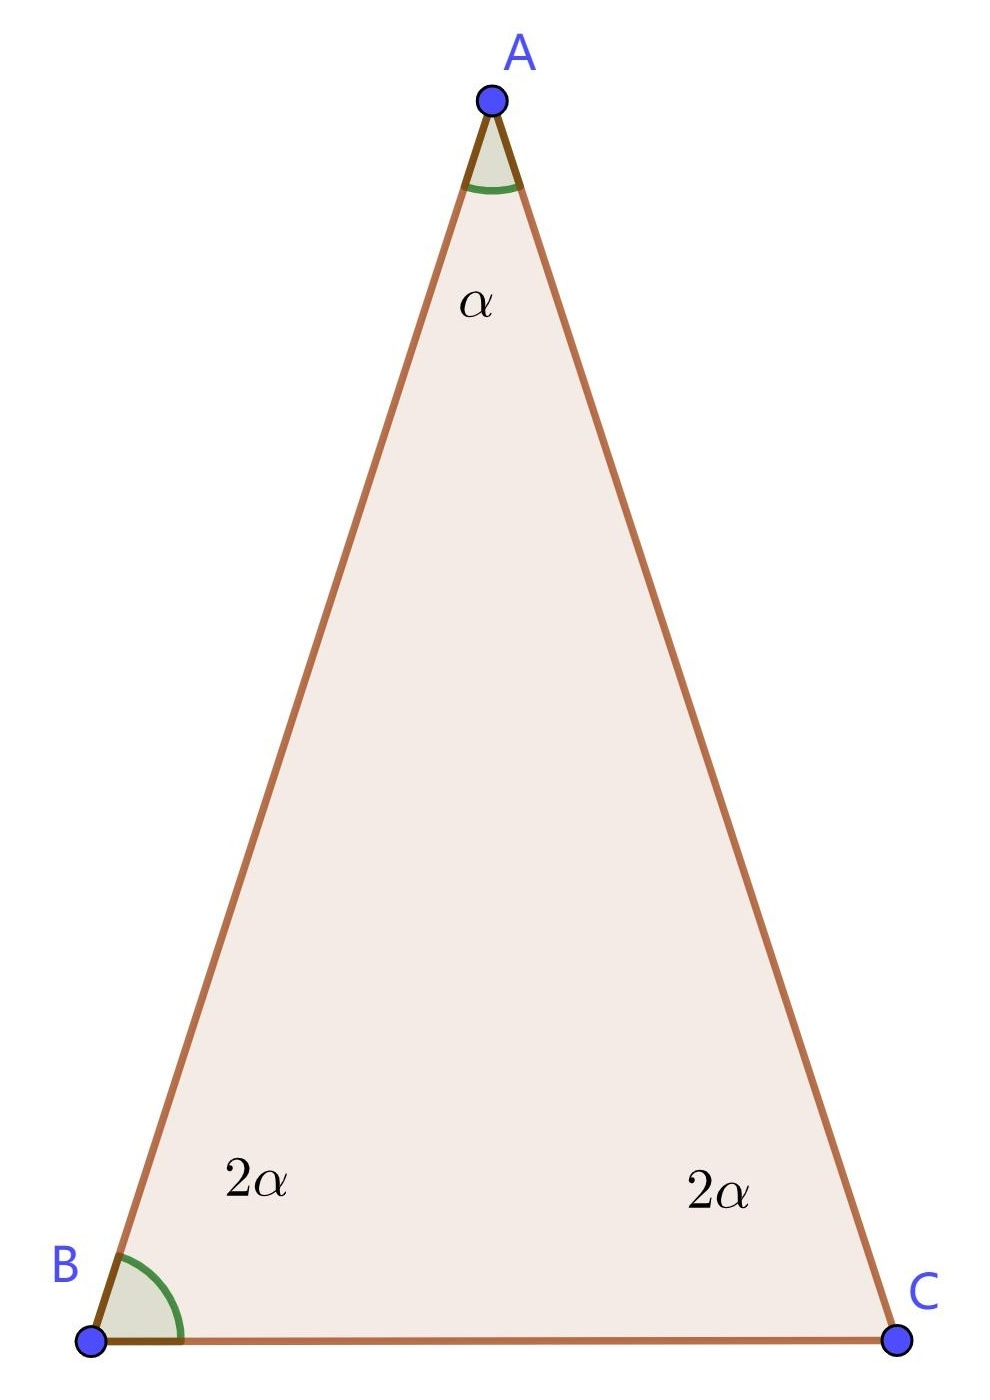
\includegraphics[scale=0.35]{img/isosceles72}
 \caption{底角为顶角2倍的等腰三角形}
 \label{fig:isosceles72}
\end{figure}

如果做两底角各自的平分线,则获得了5个$36\degree$。但做正五边形需要平分$360\degree$为5份,而不是平角$180\degree$为5份。这很容易解决,因为圆心角是圆周角的二倍。所以\cref{fig:triangle-pentagon}中的圆心角就是72度。而对应的5段弧都相等,因而五条弦(即五边形的边长)都相等,所得图形为正五边形。

\begin{figure}[htbp]
 \centering
 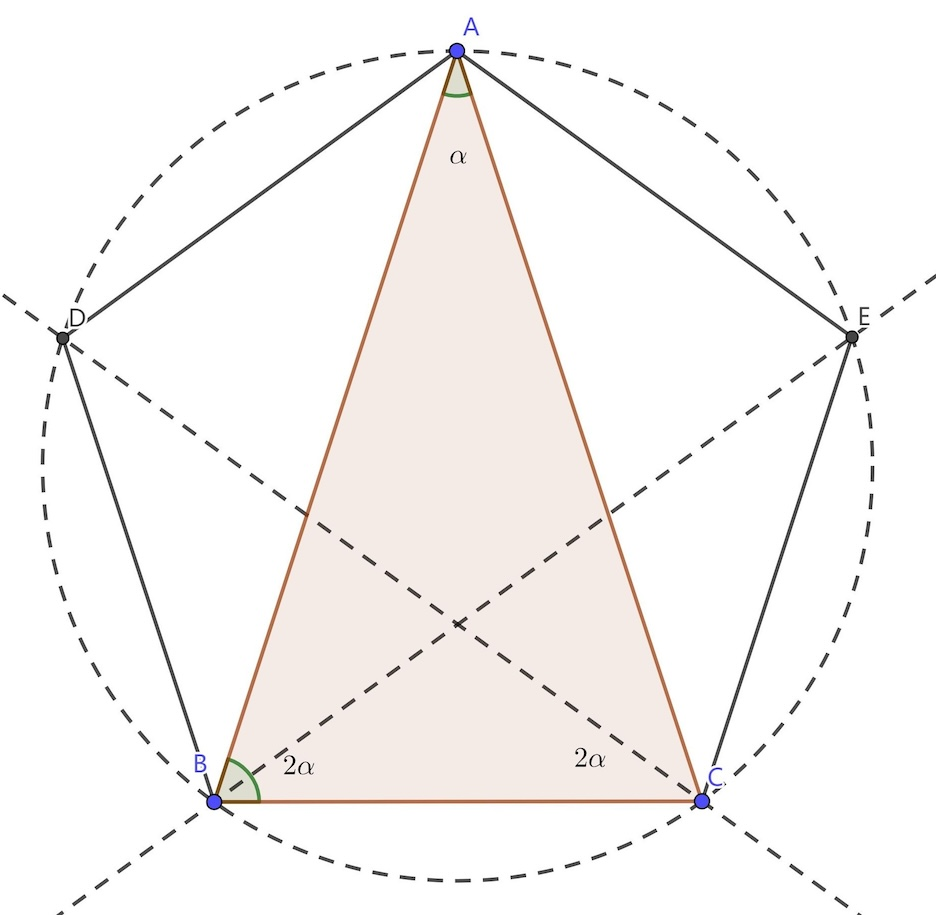
\includegraphics[scale=0.35]{img/triangle-pentagon}
 \caption{作两底角各自的平分线获得5个$72\degree$的圆周角}
 \label{fig:triangle-pentagon}
\end{figure}

\begin{proposition}[欧几里得《原本》,卷4,命题11]
在圆内可作内接正五边形。
\end{proposition}

\begin{proof}
根据此前的分析,我们只要证明可以作出顶角为$36\degree$的等腰三角形。由\cref{fig:triangle-pentagon}知,这个等腰三角形的底和腰之比(即BC:AB)恰好是正五边形的边长和对角线之比。而由第\ref{sec:pentagon-edge}节知,此比例为黄金比$\phi = \dfrac{\sqrt{5} - 1}{2}$。接下来就和方法1类似了:(1) 构造边长为$\dfrac{1}{2}$和1的直角三角形,由勾股定理,其斜边为$\dfrac{\sqrt{5}}{2}$;再从斜边截去$\dfrac{1}{2}$即得到黄金比$\phi$。(2) 利用$1, \phi, 1$作等腰三角形ABC,其顶角为$36\degree$。作此三角形的外接圆。(3) 分别作等腰三角形底角的平分线,交外接圆于D和E点。依次连接A, B, C, D, E得正五边形。
\end{proof}

第5章中我们会再给出一种利用复数和棣莫佛定理作正五边形的方法。这样正五边形尺规作图的问题得以解决了。可是接下来正7边形难住了古希腊人,人们一直没有找到它的尺规作图方法。时光跨越了两千多年。1792年,一个15岁的少年正在踌躇于下一步的人生决定。他生于德国不伦瑞克一个普通人的家庭,母亲是一位贫穷石匠的女儿,虽然十分聪明,但却没有接受过教育,近似于文盲。父亲曾做过园丁。尽管家里很穷,父亲也不认为学问有何用,但他依旧喜欢看书。童年的时候,冬天吃完饭后父亲就会要他上床睡觉,以节省燃油,但他把蔓菁的内部挖空,塞入棉布卷,当成灯来使用,以继续读书。在9岁的时候,这孩子已经找出了计算1到100求和的方法:$1 + 100 = 2 + 99 = \dotso = 50 + 51 = 101$,一共50个101。这让他的老师极为惊异。这位神童惊动了不伦瑞克公爵,决定资助他接受教育。15岁时,他犹豫应该在未来从事神学还是研究数学。这一年他证明了正17边形可以用尺规作出\cite{Gauss-Britannia-2025},他极为兴奋和自豪,从此定下了投身数学的决心。这位少年就是数学王子高斯。

\begin{figure}[htbp]
 \centering
 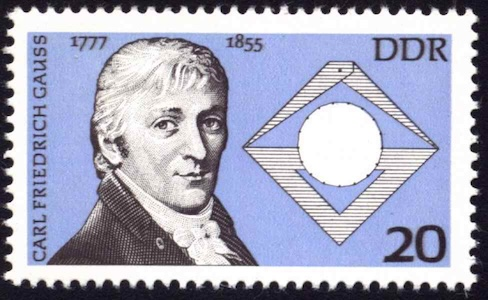
\includegraphics[scale=0.5]{img/gauss-17gon}
 \caption{高斯解决正17边形尺规作图的纪念邮票}
 \label{fig:gauss-17gon}
\end{figure}

我们这里跳过了正17边形具体的作图方法。1832年,两位数学家给出了正257边形的作图方法。德国哥廷根大学的图书馆至今保存着一大箱子正65537边形作图过程的稿纸\citepage[27页]{Coxeter2022},它耗费了作者赫爱马仕\footnote{Hermes,约翰·古斯塔夫·爱马仕。他于1894年完成了65537边形的尺规作图法。}整整10年的努力。且慢,这些数字怎么看着这么熟悉?正三角形能作出,$3 = 2^{2^0} + 1$;正五边形能作出,$5 = 2^{2^1} + 1$,正17边形能作出,$17 = 2^{2^2} + 1$;正257边形能作出,$257 = 2^{2^3} + 1$;正65537边形能作出,$65537 = 2^{2^4} + 1$。它们竟然是费马数!而且一旦能作出正$n$边形,通过中垂线二分就能作出正$2n$边形。那么正$2^k m$边形能否作出,取决于正$m$边形能否作出,其中$m$是奇数。这就是高斯的发现:如果$m$是不同的费马素数的乘积,那么这样的正多边形就能用尺规作出。法国数学家旺策尔于1837\footnote{皮埃尔·旺策尔这一年只有23岁,他英年早逝,34岁时死于过量的工作,无规律的生活和吸食鸦片。}年证明了高斯的发现,今天这一定理被称做高斯——旺策尔定理。

\begin{theorem}[高斯——旺策尔]
正$p$边形,其中$p$为素数,可以用尺规做出的条件是$p=2^{2^n} + 1$ ,即素数$p$为费马数。正$n$边形可以用尺规做出的条件是$n=2^k p_1 p_2 \dotsm p_m$其中$p_i$是不同的费马素数\cite{Edward-1977}。
\end{theorem}

\subsection{尺规的限制}
高斯——旺策尔定理告诉我们尺规作图的能力是有边界的,而不是万能的。例如正七边形的边长线段是无法用尺规作图构造出的\footnote{我们这里限制为古希腊的无刻度直尺和圆规,使用其它工具,包括有刻度的尺子是可能作出的。}。既然尺规能实现算术运算和开二次方根,那么正七边形的边长显然不能用有理数的加减乘除、开二次方根等一系列运算计算出来。它是一个无理数,但我们不知道如何用算术方法表示它。借助三角函数,当正七边形的外接圆半径为1时,其边长为$x = 2\sin(\dfrac{180\degree}{7})$,如\cref{fig:heptagon}所示。

\begin{figure}[htbp]
 \centering
 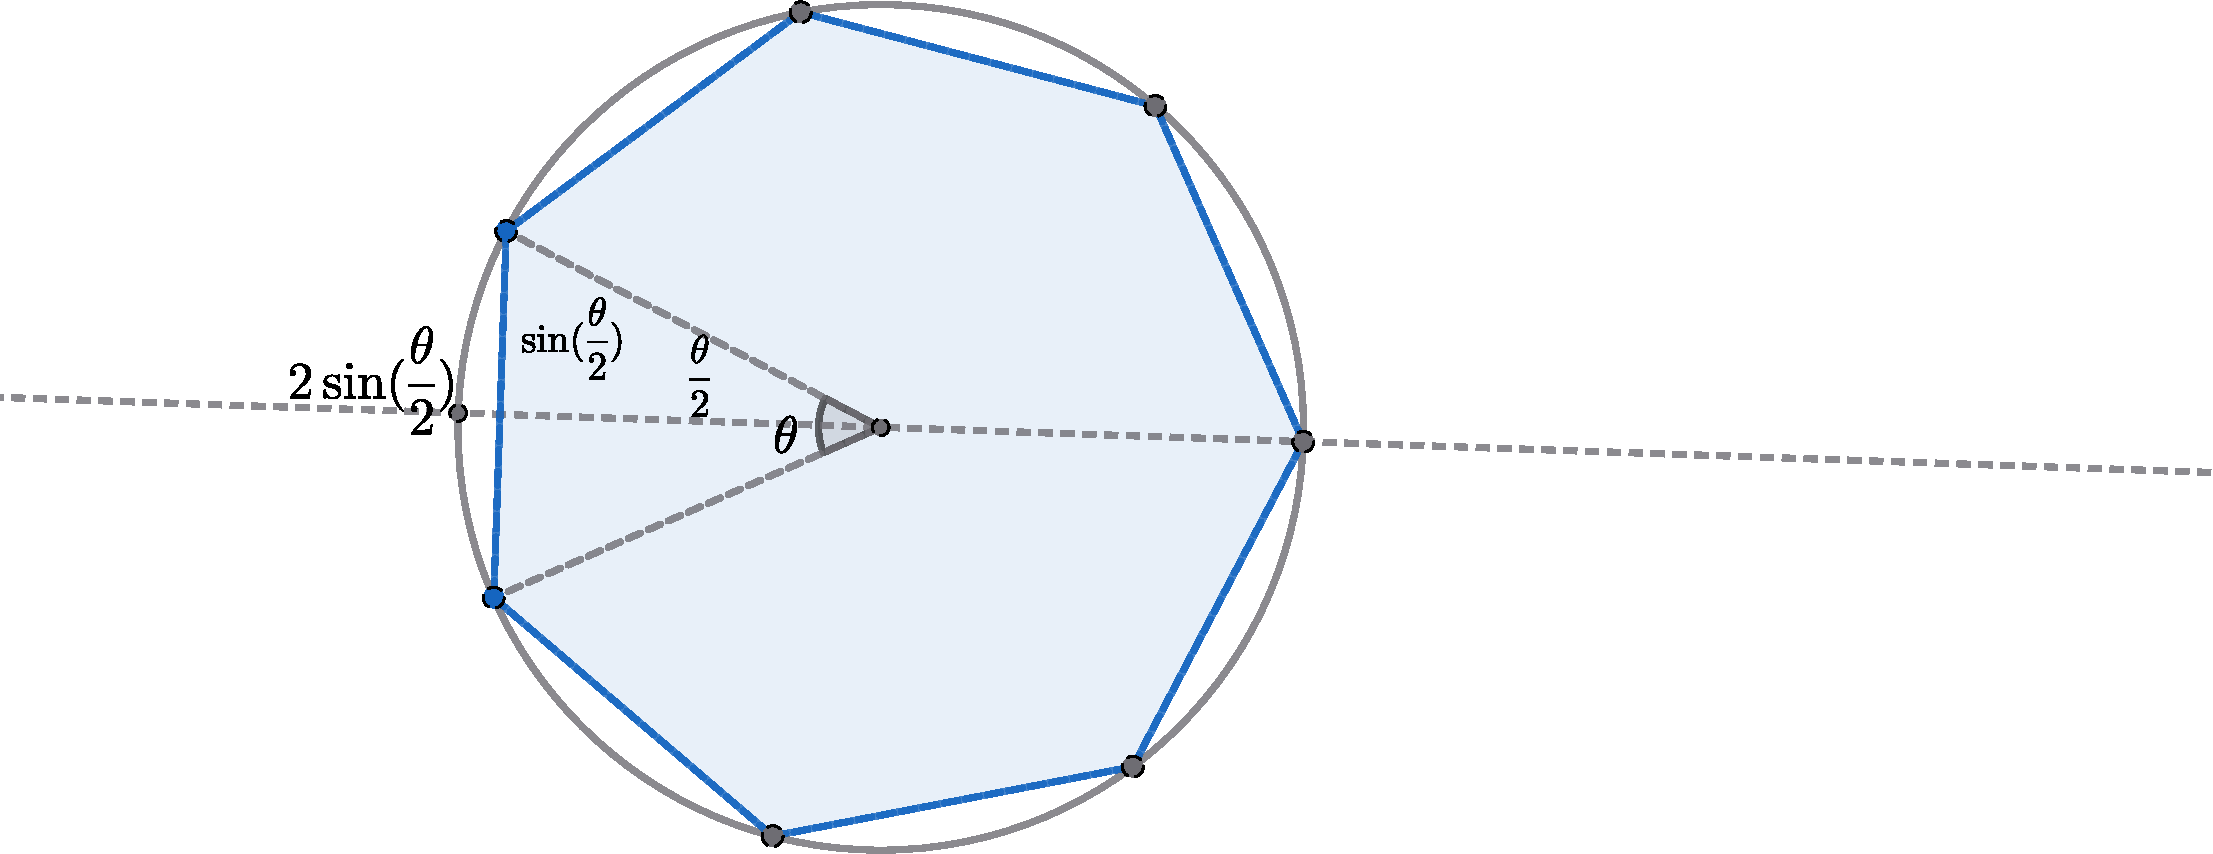
\includegraphics[scale=0.35]{img/heptagon}
 \caption{用三角函数表示正七边形的边长。外接圆半径为1,正七边形将圆周角$360\degree$分成7份,$\theta = \dfrac{360\degree}{7}$,其一半的正弦为$\sin(\dfrac{180\degree}{7})$,它恰好是边长的一半。}
 \label{fig:heptagon}
\end{figure}

古希腊人并不知道这一点,他们坚守柏拉图立下的传统,坚持用尺规探索世界。他们攻克了一个又一个的问题,但也困惑于著名的三大作图问题:

\begin{enumerate}[(1)]
\item 倍立方。将立方体的体积扩大到2倍。传说古代雅典城爆发了瘟疫,众人到阿波罗神庙祈求太阳神的帮助。祭司说阿波罗要求把立方体祭坛扩大到2倍以消除灾难。这难倒了人们。用今天的语言描述,若原立方体的边长为1,倍立方问题就是用尺规作长为$\sqrt[3]{2}$的线段。

\item 三分角。任给一个角度$\theta$,作其三等分角$\dfrac{\theta}{3}$。注意,有些特殊的角可用尺规三分,如$90\degree$、$135\degree$、$180\degree$、$360\degree$,但一般的角$\theta$不可三分,例如$60\degree$。

\item 圆化方。求作正方形,使得其面积等于给定圆的面积。若圆的半径为1,就是求边长为$\sqrt{\pi}$的正方形。
\end{enumerate}

直到十九世纪,伴随着抽象代数,特别是域论、群论、伽罗瓦理论的发展,人们才最终解决了古希腊三大作图问题——它们的答案都是否定的,即不存在尺规作图方法可以倍立方、三分角、圆化方\footnote{倍立方和三分角都由旺策尔解决,圆化方本质是证明$\pi$是一个超越数,1882年由德国数学家林德曼证明。}。

尽管高斯——旺策尔定理的证明需要抽象代数和域论的知识,但我们可以给出一个大致的原理性解释(附录\ref{app:gauss-wantzel-theorem}给出了一个证明梗概)。十七世纪,笛卡尔创造了解析几何(英文analytic geometry,也称做坐标几何,英文coordinate geometry),重新将几何建立在代数(方程和函数)的基础上。古希腊的尺规作图也有了全新的代数解释。

\subsubsection{两点确定一直线}
平面上的一条直线可以用函数$y = kx + b$描述,其中$k$是斜率,$b$是截距,特殊直线为$x = a$。欧几里得几何的公设1,过两点可作一直线。其对应的解析几何解释为:连接不同的两点$(x_1, y_1)$和$(x_2, y_2)$得到一条直线(其中$x_1 \ne x_2$)。这两点都满足直线方程:

\[
\begin{cases}
y_1 = k x_1 + b \\
y_2 = k x_2 + b
\end{cases}
\]

解此二元一次方程组可求出$k$和$b$。两式相减得$k = \dfrac{y_2 - y_1}{x_2 - x_1}$,代回可求出$b = y_1 - k x_1$。我们也可以直接使用“两点式”得到这条直线方程(见\cref{fig:line2p}):

\[
\frac{y - y_1}{x - x_1} = \frac{y_2 - y_1}{x_2 - x_1}
\]

\begin{figure}[htbp]
 \centering
 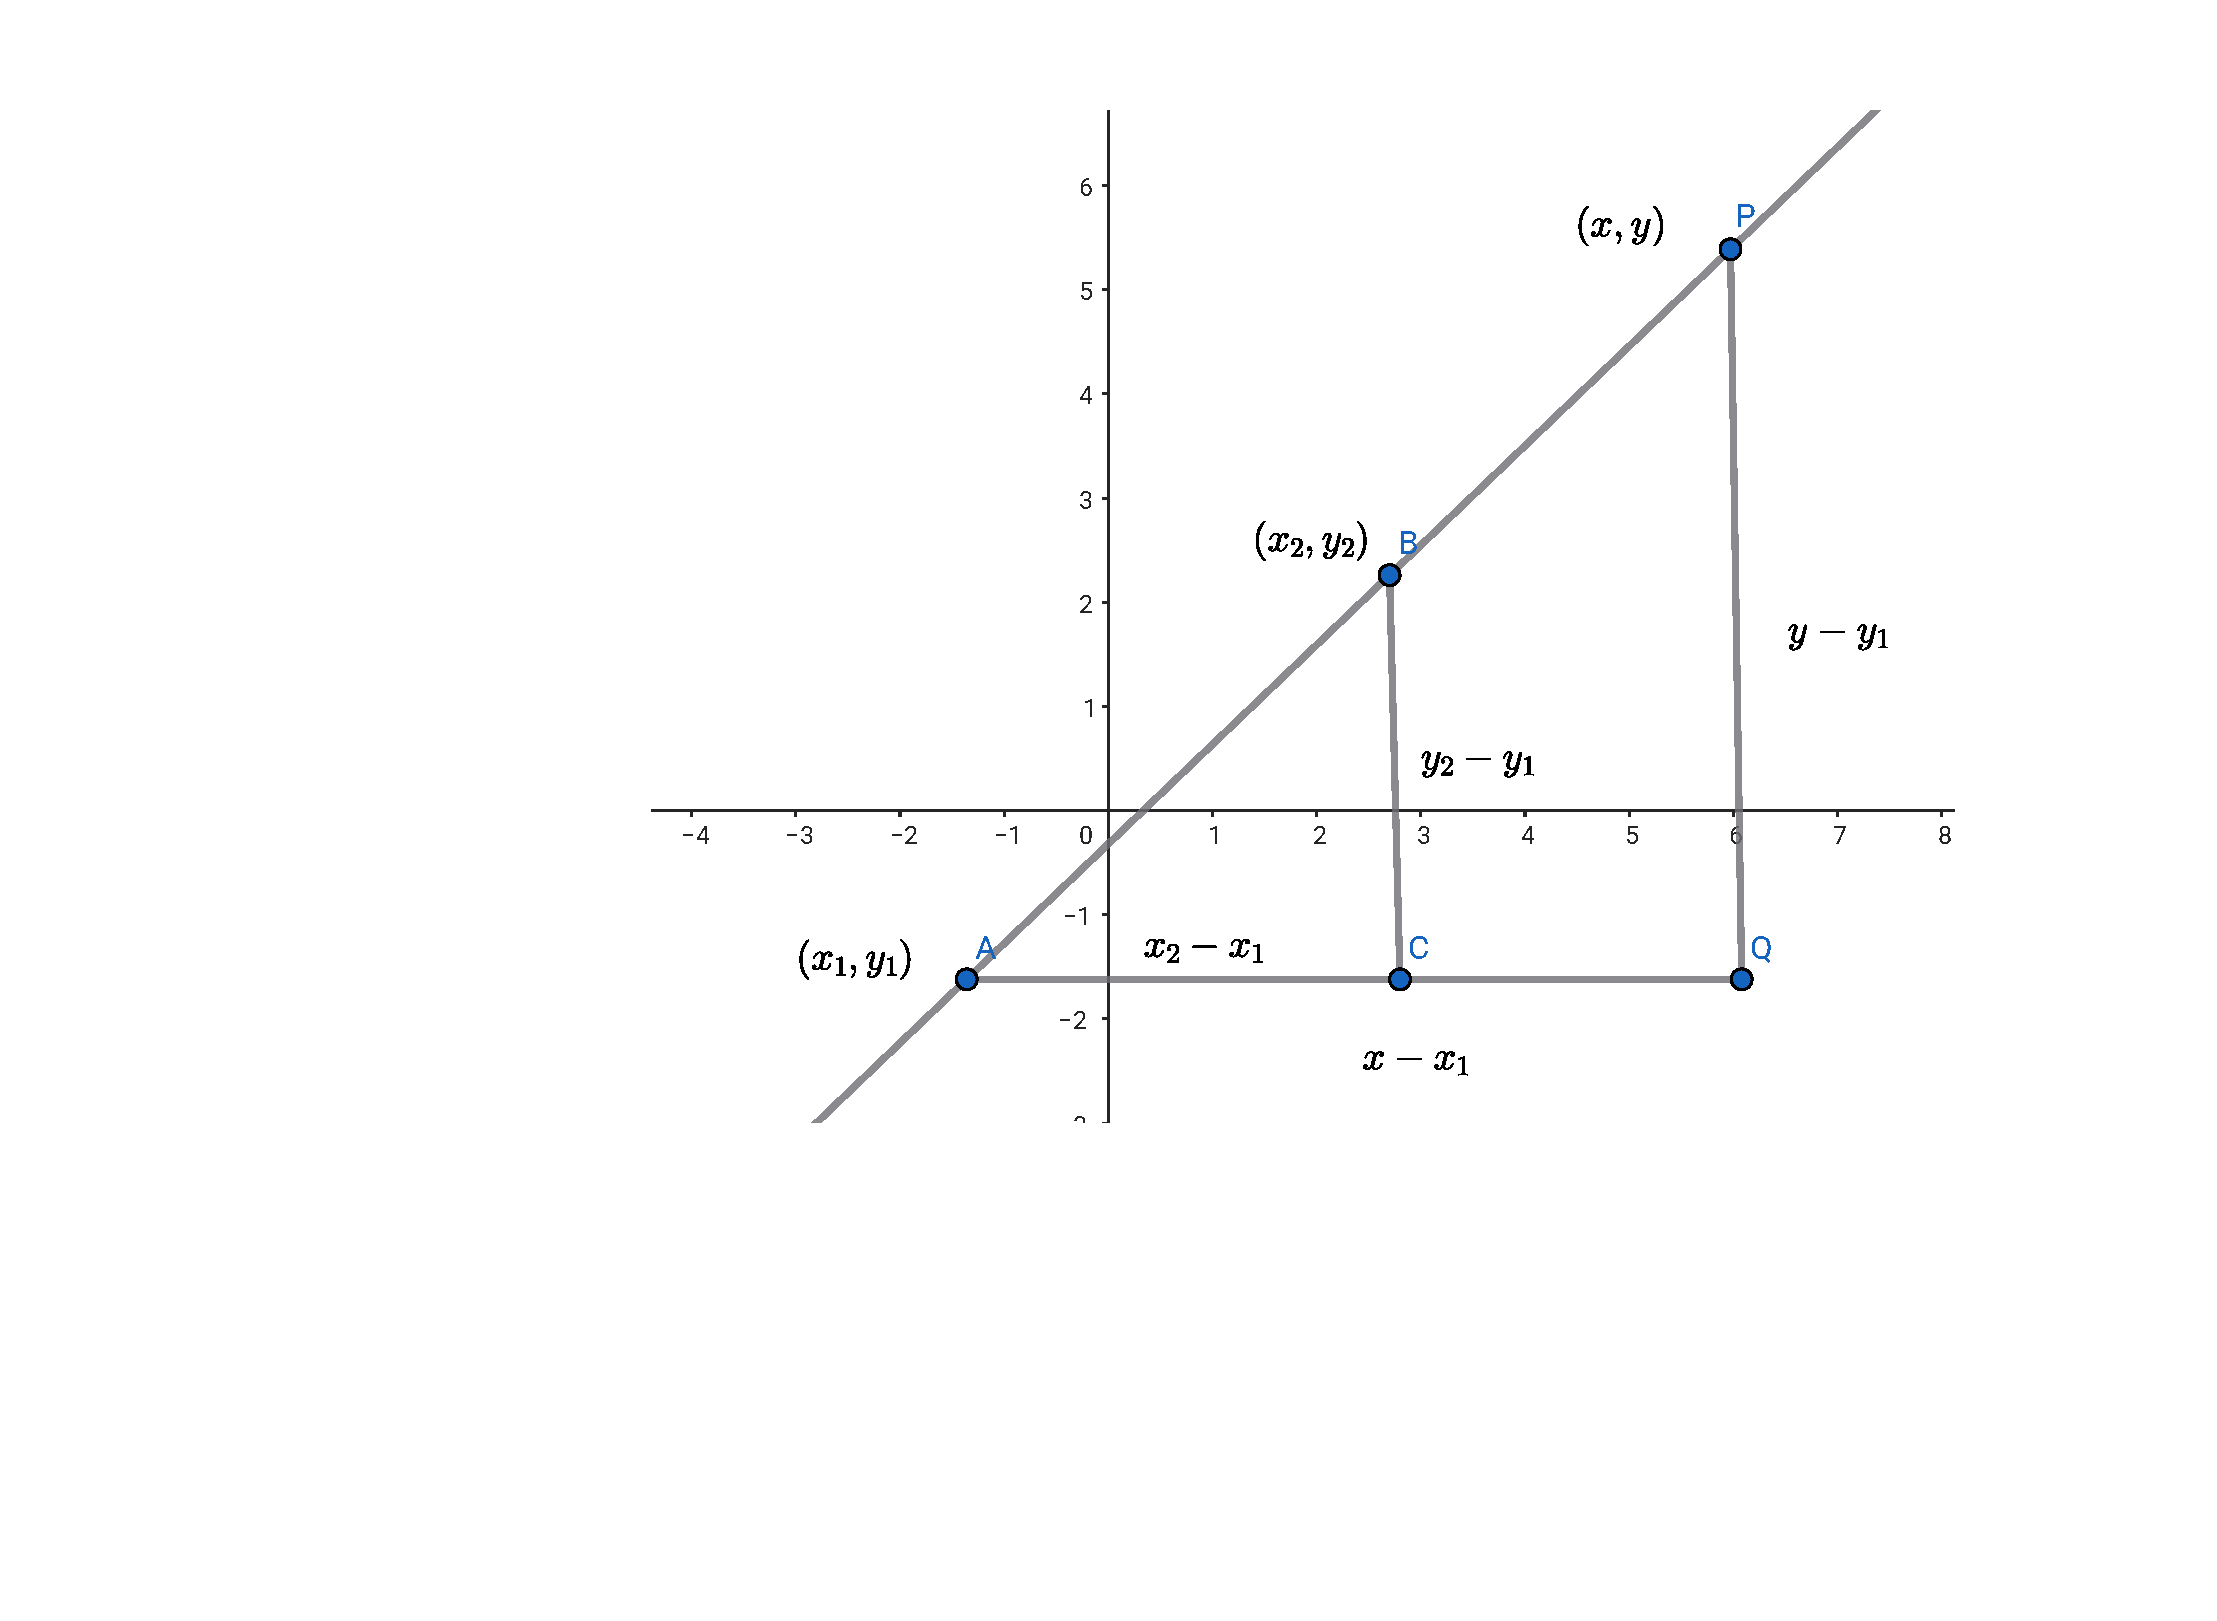
\includegraphics[scale=0.35]{img/line2p}
 \caption{两点式的几何解释:连接两点$A, B$成一直线,$P = (x, y)$为直线上任意一点。直角三角形ACB和AQP相似,所以$\dfrac{PQ}{QA} = \dfrac{BC}{CA}$。}
 \label{fig:line2p}
\end{figure}

若$x_1 = x_2$,则连接两点的直线是函数$x = x_1$。记这两点确定的线段的长为$r$,根据勾股定理$(x_2 - x_1)^2 + (y_2 - y_1)^2 = r^2$,得$r = \sqrt{(x_2 - x_1)^2 + (y_2 - y_1)^2}$。长度$r$是一个二次根式,它是勾股定理确定的一元二次方程(未知数为$r$)的解。总结起来,两点确定一条直线本质上是说:若两点坐标中的数属于数集$K$(例如$K = \mathbb{Q}$是有理数,$K$也可以是比有理数更大的数集),则其确定的直线是系数为$K$的一次函数。这两点的距离是系数为$K$的一元二次方程的解。

顺便说一下,过一点作另一直线的垂线的解析几何解释。与直线$y = kx + b$垂直的直线具有$y = -\dfrac{1}{k} x + b'$的形式,其中$k \ne 0$。若垂线过点$(x_0, y_0)$,则:$y_0 = -\dfrac{1}{k} x_0 + b'$,从中得到$b' = y_0 + \dfrac{1}{k}$。与特殊直线$x = a$垂直的直线具有$y = b$的形式,若垂线过点$(x_0, y_0)$,则确定出的垂线方程为$y = y_0$。总结起来,若给定直线的斜率和通过的点属于数集$K$,则其确定的垂线是系数是为$K$的一次函数。

\subsubsection{点和半径确定一个圆}

欧几里得几何公设3说:以任意点为圆心及任意的距离可以画圆。平面上给定三点$O, M, N$,以$O$为圆心,线段$MN$的长度为半径,可以唯一确定一个圆。其中半径$r = \sqrt{(x_m - x_n)^2 + (y_m - y_n)^2}$,是通过$M, N$的坐标和勾股定理确定的长度。我们从高中的解析几何中知道圆心为$(a, b)$,半径为$r$的圆可用方程$(x - a)^2 + (y - b)^2 = r^2$来描述。总结起来,若三点的坐标属于数集$K$,则其确定的圆是系数为$K$的二次方程。

\subsubsection{交点}
交点有三种:直线与直线的交点,直线与圆的交点,圆与圆的交点。两直线的交点是二元一次方程组

\[
\begin{cases}
y = k_1 x + b_1 \\
y = k_2 x + b_2
\end{cases}
\]

的解。若两直线不平行($k_1 \ne k_2$)则解是唯一的,交点唯一确定。若$k_1 = k_2$,但$b_1 \ne b_2$,则两直线平行,没有交点,方程组无解。若$k_1 = k_2$且$b_1 = b_2$,两直线重合。交点有无穷多。总之,不平行的直线有交点,若直线方程的系数属于数集$K$,则交点的坐标也属于数集$K$。

直线和圆的关系可用方程组

\[
\begin{cases}
(x - a)^2 + (y - b)^2 = r^2 \\
y = kx + c
\end{cases}
\]

的解来确定。把第二式代入第一式可得一元二次方程

\begin{align*}
& (x - a)^2 + (kx + c - b)^2 = r^2  &&\text{代入}y = kx + c \\
& x^2 + a^2 - 2ax + k^2x^2 + d^2 + 2kdx - r^2 =0 && \text{令}d = c - b \\
& (1 + k^2)x^2 + 2(kd - a)x + a^2 + d^2 - r^2 = 0 && \text{合并同类项} \\
& Ax^2 + 2Bx + C = 0
\end{align*}

其中$A = 1 + k^2, B = kd - a, C = a^2 + d^2 - r^2$, 它的判别式$\Delta = \sqrt{4B^2 - 4AC} = 2\sqrt{B^2 - AC}$。有三种情况:
\begin{itemize}
\item 若$B^2 < AC$,直线与圆相离,没有交点。
\item 若$B^2 = AC$,直线与圆相切,方程的解为切点。
\item 若$B^2 > AC$,直线与圆相割,方程的解为两交点。
\end{itemize}

两圆的关系用方程组
\[
\begin{cases}
(x - a)^2 + (y - b)^2 = r_1^2 \\
(x - c)^2 + (y - d)^2 = r_2^2
\end{cases}
\]

的解来确定。它同样能化为一元二次方程,然后用判别式$\Delta >, =, < 0$来描述两圆相离、相切、相交。总结下来,直线与圆、圆与圆的交点的坐标是二次方程的解。注意:这些方程的系数并不一定是有理数,例如\cref{fig:P1}中的直线CE对应的一次方程的斜率$k$和截距$b$都不是有理数。

至此,尺规作图的能力范围已经全被笛卡尔掌握并定义出了。在平面上给定两个点A和B,我们指定其中一个为原点$(0, 0)$,另一个为$(1, 0)$。这两点就确定了长度为1的单位线段。我们可以进行第一轮尺规作图,包括:(1) 连接所有的已知点得到一组直线$\mathbf{L}_1$; (2) 以所有的已知点为圆心,已知线段为半径作一组圆$\mathbf{C}_1$;(3) 作所有不平行直线的交点,所有直线和圆的交点、切点,所有圆彼此间的交点和切点,记这些点为$\mathbf{P}_1$。

\begin{figure}[htbp]
 \centering
 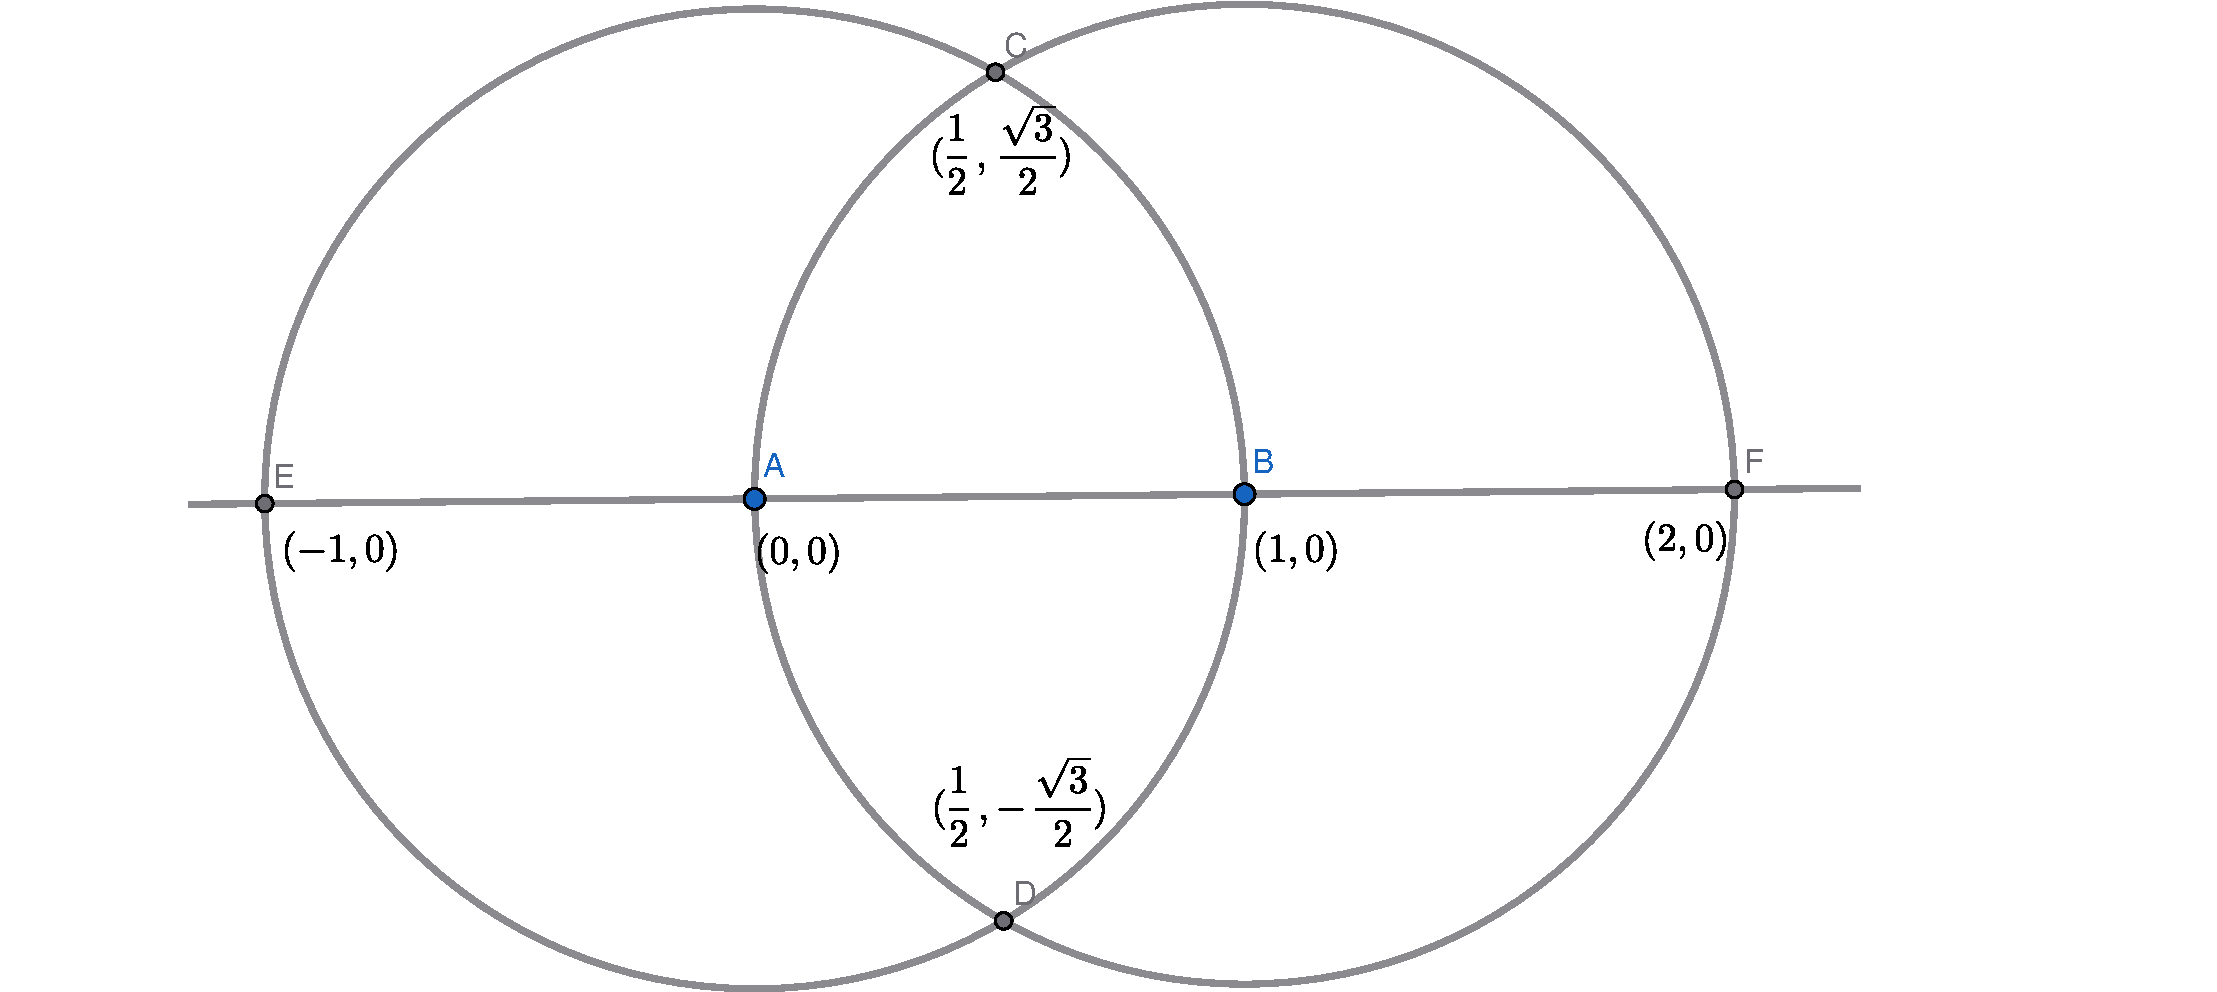
\includegraphics[scale=0.35]{img/P1}
 \caption{第一轮尺规作图后得到的点$\mathbf{P}_1 = \{A, B, C, D, E, F\}$}
 \label{fig:P1}
\end{figure}

如\cref{fig:P1}所示,第一轮尺规作图后获得1条直线,两个圆,6个点。\underdot{所有}可能作出的长度,无非是系数为有理数的一元一次方程和一元二次方程的解,记为$K_1$。接下来在此基础上进行第二轮尺规作图,同样包括三部分:(1) 连接$\mathbf{P}_1$中所有任意两点得到的一组直线$\mathbf{L}_2$; (2) 用$\mathbf{P}_1$中所有任意三点$O, M, N$作圆,圆心为$O$,半径为线段$MN$的长度,这样得到一组圆$\mathbf{C}_2$;(3) 所有$\mathbf{L}_2$中直线的交点,所有$\mathbf{L}_2$中的直线与所有$\mathbf{C}_2$中圆的交点、切点,所有$\mathbf{C}_2$中圆彼此间的交点、切点,记这些点为$\mathbf{P}_2$。

第二轮尺规作图能作出的量,是以$K_1$为系数的一元一次方程和一元二次方程的解,记为$K_2$。重复这一步骤,我们可以一轮一轮进行尺规作图,从而得到越来越多尺规可作出的量$K_1, K_2, K_3, \dotsc$其中包括这样的数:$1 + \sqrt{2} + \sqrt{2\sqrt{3} - \sqrt{5}}$等等。读者朋友们,你能举出更多的例子么?

尺规可作数的集合,随着轮数的增加,规模以指数爆炸的形式增加。一轮一轮无穷无尽,不断以上一轮的数为系数组成新的一元一次方程和一元二次方程,它们的解构成下一轮的数。它是一个无穷集合,尽管如此$\sqrt[3]{2}$却不在其中。它不是任何以有理数为系数的一次或二次方程的解;它不是任何以$K_1$为系数的一次或二次方程的解;它不是任何以$K_2$为系数的一次或二次方程的解……它是尺规不可作的\footnote{$\sqrt[3]{2}$是三次方程$x^3 - 2 = 0$的唯一实根,另外两个根是复数$-\sqrt[3]{2}\dfrac{1 \pm \sqrt{3}}{2}$,详见第5章。}。这就是倍立方问题无法解决的原因。如\cref{fig:heptagon}所示,正$n$边形的边长为$x = 2\sin(\dfrac{360\degree}{2n})$。如果它是某个$K_i$中的一次或二次方程的解,则尺规可作出,否则尺规不可作出。

由高斯——旺策尔定理,正18边形用尺规不可作出($18 = 2 \times 3^2$,不是不同的费马素数与2的幂的积),所以$360\degree$角的$\dfrac{1}{18}$,即$20\degree$不可作出,进一步可知$60\degree$角无法用尺规三等分。这样就推翻了三分角问题。

\begin{figure}[htbp]
 \centering
 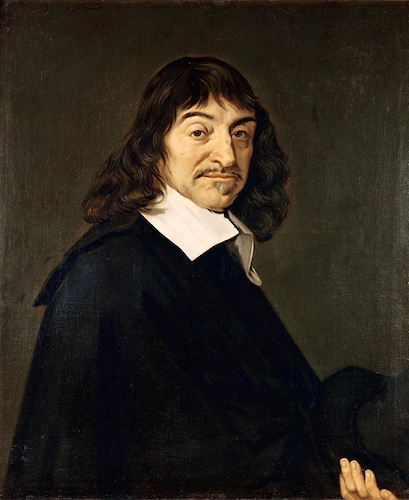
\includegraphics[scale=0.4]{img/Descartes}
 \caption{哈尔斯创作的画布油画:勒内·笛卡尔(1596-1650)。现藏于卢浮宫}
 \label{fig:Decartes}
\end{figure}

\index{笛卡尔}
\begin{mdframed}
笛卡尔是法国哲学家、数学家、物理学家。在笛卡尔的时代,拉丁文是学术上广泛使用的语言。笛卡尔也有一个拉丁化的名字——卡提修斯(Cartesius)。正因为如此,笛卡尔坐标系也称卡氏坐标系。

笛卡尔1596年生于法国一个地位较低的贵族家庭。一岁时他的母亲患肺结核去世,而他也受到传染,造成体弱多病。母亲去世后,父亲移居他乡并再婚,笛卡尔由外祖母带大,自此父子很少见面,但是父亲一直提供金钱方面的帮助,使他能够受到良好的教育。笛卡尔后来进入位于拉弗莱什的耶稣会的皇家大亨利学院学习。在那里,他学习到了数学和物理学,包括伽利略的工作。由于笛卡尔体弱多病,学校特许他每天早上不用像其他同学一样5点起床,而是一直睡到11点。笛卡尔直到晚年仍然保留了这一作息习惯。1614年毕业后,他遵从父亲的意愿,进入普瓦捷大学学习法律,并获得业士学位和文凭。毕业后笛卡尔一直对职业选择不定,又决心游历欧洲各地,专心寻求“世界这本大书”中的智慧。1618年,笛卡尔加入荷兰拿骚的毛里茨军队。笛卡尔对数学与物理学的兴趣,是在荷兰当兵期间产生的。1618年,他偶然在路旁公告栏上,看到用佛莱芒语提出的数学问题征答。这引起了他的兴趣,并且让身旁的人,将他不懂的佛莱芒语翻译成拉丁语。这位身旁的人就是大他八岁的以撒·贝克曼(Isaac Beeckman)。贝克曼在数学和物理学方面有很高造诣,很快成为了他的导师。4个月后,他写信给贝克曼:“你是将我从冷漠中唤醒的人……”。

1622年,26岁的笛卡尔变卖掉父亲留下的资产,用4年时间游历欧洲。他先在意大利住了2年,随后迁往巴黎。当时法国教会势力庞大,不能自由讨论宗教问题,因此笛卡尔在1628年移居荷兰,在那里住了20多年。他深居简出,仅仅通过好友梅森和学术界取得联系。在此期间,笛卡尔致力于哲学研究,他发表了多部重要的文集,包括《方法论》、《形而上学的沉思》和《哲学原理》等,成为欧洲最有影响力的哲学家之一。1637年,笛卡尔在他的文章《几何学》中,创立了解析几何。

1649年笛卡尔受瑞典克里斯蒂娜女王之邀来到斯德哥尔摩担任女王的私人教师。但是女王习惯在清晨5点起床向笛卡尔学习,这一下子打破了笛卡尔一生11点起床的作息习惯。几个月后,在这片“熊、冰雪与岩石的土地”上,笛卡尔不幸得了肺炎,在1650年2月去世,享年54岁。笛卡尔留下名言“我思故我在”,提出了“普遍怀疑”的主张。这是一句常被误解的话,“我思故我在”译自拉丁文cogito ergo sum,直译过来是:“思考时自我是存在的。”笛卡尔观察到人的感觉靠不住。海市蜃楼看似真实,其实不存在。为了追求真理,他先假定所有的事物都不存在,然后通过理性证明、判断哪些事物存在。在这一思考过程中,笛卡尔认识到,作为思维主体的自我必定存在。这就是“我思故我在”的真正含义。他开拓了欧洲理性主义哲学,是西方现代哲学的奠基人。他的哲学思想深深影响了之后的几代人。笛卡尔对现代数学的发展做出了重要的贡献,他创立的解析几何,成功地将当时完全分开的代数和几何学联系到了一起。
\end{mdframed}

\section{圆周率}
圆周率$\pi$是数学课上的老朋友。我们无从知道人类最早什么时候认识到圆周与直径的比值是固定的,也许这来自测量的经验。\cref{fig:ybc7302}是耶鲁大学皮博迪自然博物馆中的一件藏品,编号YBC7302。这是古巴比伦时代(约公元前1900年~前1600年)的泥板,上面刻有楔形数字(见第1章)。\cref{fig:proust-ybc7302}是法国历史学家普鲁斯特绘制的示意图\cite{Proust-2016}。在圆周上刻有数字3,园内刻有数字45,圆外右侧刻有数字9。我们知道古巴比伦采用60进制,普鲁斯特据此给出了这幅图的数学解释:3是周长,9是周长的平方。我们知道周长是$C = 2\pi r$,其中$r$是半径。周长的平方是$4\pi^2 r^2$,所以面积和周长的关系是:

\begin{figure}[htbp]
 \centering
 \subcaptionbox{耶鲁大学收藏的古巴比伦圆形泥板,刻有圆形和楔形数字,涉及圆的周长和面积。\label{fig:ybc7302}}{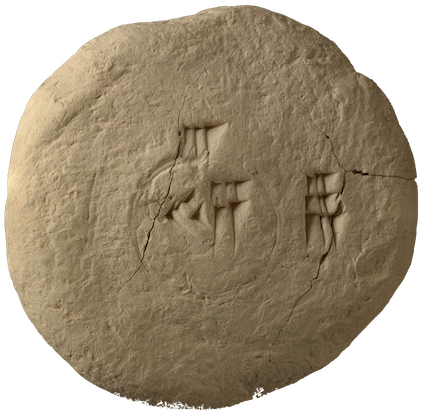
\includegraphics[scale=0.4]{img/ybc7302}}
 \subcaptionbox{楔形数字3、9、45\label{fig:proust-ybc7302}}{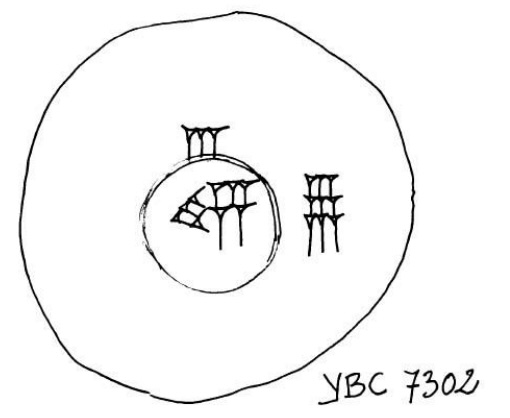
\includegraphics[scale=0.5]{img/proust-ybc7302}}
\end{figure}

\[
S = \pi r^2 = \frac{4 \pi^2 r^2}{4\pi} = \frac{C^2}{4\pi}
\]

按照$\pi \approx 3.14$计算,$S = 9/4\pi \approx 0.72$,那么45怎么解释呢?虽然古巴比伦采用位值制计数系统,但没有零和小数点,这里就造成了麻烦。其实这里是60进制0.45,即十进制$\dfrac{45}{60} = 0.75$。这样我们可以反推出古巴比伦人使用的圆周率数值:

\[
\pi = \frac{C^2}{4S} = \frac{9}{4 \times 0.75} = 3
\]

古人很快就不满足这个精度了。在古埃及的莱茵德纸草书中(约公元前1650年),第50题是关于圆面积的:如果一个圆形田地的直径是9凯特(khet),面积是多少?作者阿梅斯给出的解答是这样的:去掉直径的$\frac{1}{9}$(也就是1),得到8。8乘以8得到64,因此面积是64赛塔特(setat)。我们据此可以反推出古埃及人使用的圆周率:

\begin{align*}
S & = \pi r^2 = \pi (\frac{d}{2})^2 \\
\pi & = 4\frac{S}{d^2} = 4(\frac{8}{9})^2 \approx 3.16
\end{align*}

\subsection{割圆术}
在人们不断寻找更精确的圆周率时,古希腊伟大的数学家阿基米德首先给$\pi$限制了范围。通过古埃及人的计算,我们可以大致推测:

\begin{proposition}
圆周率$\pi$在3和4之间。
\end{proposition}

在小学数学课上,我们曾经在老师的指导下用线绳、直尺测量圆的周长和直径,感知圆周率的存在。$3.14$成为了每个人儿时的机械记忆,它自然是在3和4之间,为什么还要证明呢?这就是古希腊几何的精神所在——追求严密和完美,并在此过程中发展工具和方法。正是通过对圆周率范围的严格界定,阿基米德取得了更好的结果并给后人指出了方向。

\begin{proof}
我们先证明$\pi > 3$。如\cref{fig:inscribed-hexagon}所示,考虑半径为1的单位圆和内接正六边形。连接正六边形的顶点和圆心将其分割为6个正三角形(首先每个三角形是等腰三角形,其中腰是圆的半径;其次每个等腰三角形的顶角等于$\frac{360\degree}{6} = 60\degree$)。由于单位圆的半径是1,所以每个等腰三角形的边长是1,所以正六边形的周长是6。由外接圆周长大于正六边形周长6,故:

\begin{figure}[htbp]
 \centering
 \subcaptionbox{半径为1的单位圆与内接正六边形\label{fig:inscribed-hexagon}}{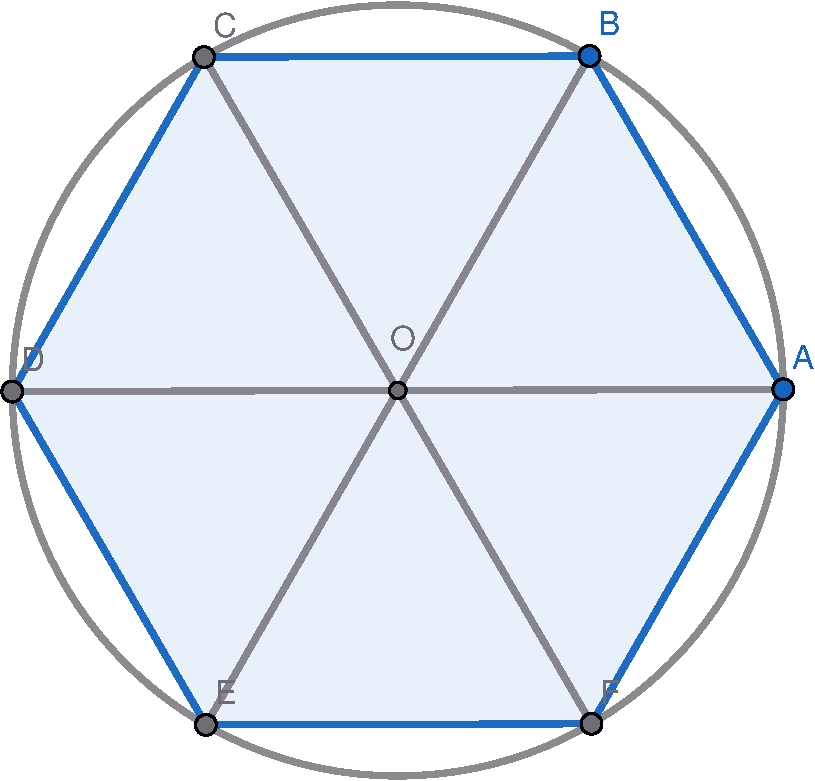
\includegraphics[scale=0.4]{img/hexagon}}
 \subcaptionbox{半径为1的单位圆与外切正方形\label{fig:square-hexagon}}{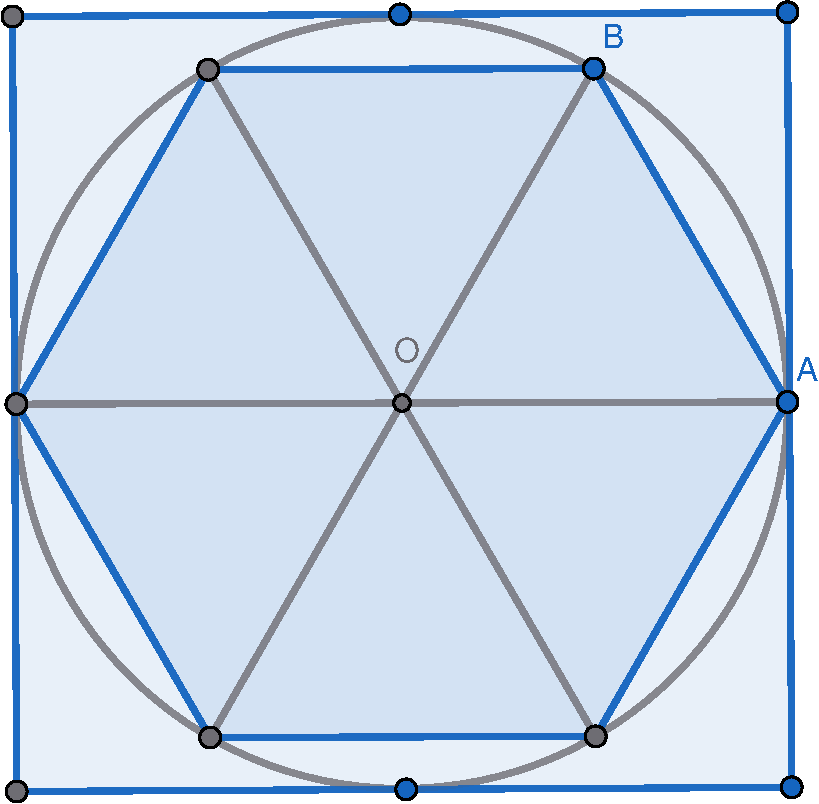
\includegraphics[scale=0.4]{img/square-hexagon}}
\end{figure}

\[
\pi = \frac{C}{d} = \frac{C}{2} > \frac{6}{2} = 3
\]

然后证明$\pi < 4$。如\cref{fig:square-hexagon}所示,进一步作外切正方形。其边长等于直径2,故正方形的周长是8。因为外切正方形的周长大于圆的周长,所以:

\[
\pi = \frac{C}{d} = \frac{C}{2} < \frac{8}{2} = 4
\]

这样就证明了圆周率$3 < \pi < 4$。
\end{proof}

这就是古希腊数学家阿基米德计算圆周率的思想,所不同的是阿基米德同时考虑圆内接和外接正多边形,如\cref{fig:pi-exhaustion}所示。取圆的直径为1,则周长等于$\pi$。圆的周长大于内接正多边形的周长而小于外切正多边形的周长。这样就有:

\begin{figure}[htbp]
 \centering
 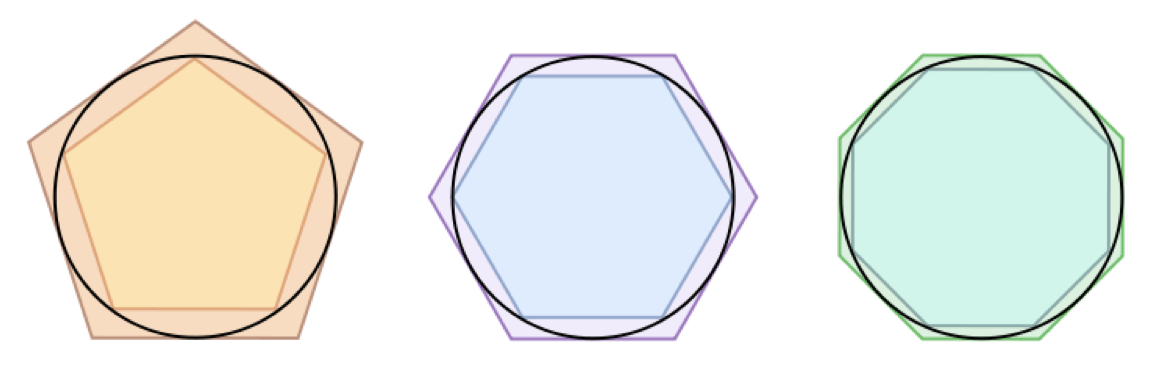
\includegraphics[scale=0.5]{img/pi-exhaustion}
 \caption{用穷竭法计算圆周率}
 \label{fig:pi-exhaustion}
\end{figure}

\[
  C_i < \pi < C_o
\]

其中$C_i$、$C_o$分别为内接多边形和外切多边形的周长。不断加大边数$n$,就可以越来越精确地获得$\pi$的范围。这种方法叫做“穷竭法”,它是在现代微积分的前驱。不管指定多么小的精度,比如$\epsilon = 0.00 \dotso 01$,我们都可以找到一个足够大的$n$,使得$C_o - \pi$和$\pi - C_i$都小于$\epsilon$。或者说当$n$趋近于无穷时,$C_o$和$C_i$都趋近于$\pi$。穷竭法由古希腊智人学派的代表人物安提丰(Antiphon,约前480~前410)首创。他提出用圆内接多边形逼近圆面积的方法来化圆为方。安提丰从一个圆内接正方形开始,不断将边数加倍得到正八边形、十六边形……不断重复这一过程,随着圆面积的逐渐“穷竭”,将得到一个边长越来越微小的圆内接正多边形。安提丰认为最终这一正多边形将与圆重合。后来古希腊数学家欧多克索斯对穷竭法进行了改进和严格化,使其成为解决面积、体积问题的一种有力的几何方法。利用穷竭法,欧多克索斯证明了棱锥体积是同底同高棱柱体积的1/3,圆锥体积是同底同高圆柱体积的1/3。这些成果都记录在欧几里得的《原本》卷12中\cite{HanXueTao16}。

古希腊将穷竭法发展到最高成就的当属阿基米德,他使用内外多边形计算出了圆周率范围:$\dfrac{223}{71} < \pi < \dfrac{22}{7}$。取上下两个边界的平均值,阿基米德相当于计算出$\pi \approx 3.1418$,误差仅有0.0002。这在没有位值制10进制计数系统的古希腊是一个极为惊人成就。今天西方仍然广泛使用$\dfrac{22}{7}$进行日常计算。除此之外,阿基米德还证明了圆面积公式,球体、锥体的表面积和体积公式,甚至找到了计算抛物线下面积的方法。被称为古希腊的数学之神。

\begin{figure}[htbp]
 \centering
 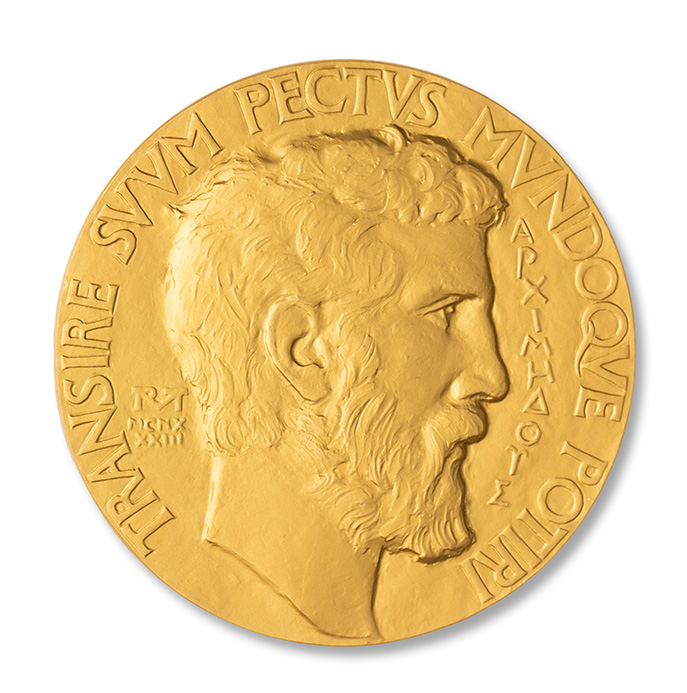
\includegraphics[scale=0.33]{img/FieldsMedal}
 \caption{菲尔兹奖章上的阿基米德像}
 \label{fig:Archimedes-book}
\end{figure}

\index{阿基米德}
\begin{mdframed}
阿基米德(前287年~前212年),生于西西里岛的叙拉古王国。早年曾经在古希腊的学术中心亚历山大城跟随欧几里得学习。阿基米德后来回到了叙拉古,他的许多学术成果都是通过和亚历山大城的学者之间的往来信件保存下来的。虽然有关阿基米德的生平没有详细的记载,但是关于他的各种故事却广为流传、脍炙人口。最著名的故事就是国王的王冠。叙拉古国王不知道他的王冠是否是纯金的,大臣们也一筹莫展,于是去请教阿基米德。阿基米德一直解不开这个难题,他废寝忘食,直到有一天洗澡的时候,看着浴缸里的水溢出来,突然得到了灵感。他从浴缸里一跃而出,光着身子跑到大街上,边跑边喊“尤里卡!尤里卡!”,这句希腊语Eureka的意思是“我找到了!”。阿基米德利用浮力和比重,最终发现王冠掺了假。他的这一发现就是每一个中学生都要学习的“阿基米德定律”。尤里卡后来被人们用来形容找到灵感的那一刹那。

阿基米德发现球的体积是其外接圆柱体积的2/3。他觉得这一关系无比的美妙,因此决定死后在墓碑上刻一个内接圆柱的球体。公元前214年,第二次布诺战争爆发了。面对敌人的围城,传说阿基米德设计了巨大的抛物面镜,把阳光汇聚到帆上烧毁了敌人的战船。阿基米德还设计了巨大的机械武器,可以瞬间击毁罗马战船。后来罗马军队攻陷了叙拉古城,一个罗马士兵冲进阿基米德家里。阿基米德正专注地在沙地上画着几何图形进行思考,他说出了那句著名的画:“你挡住了我的阳光。”感到被冒犯的罗马士兵挥刀杀死了面前的这个老人。古希腊最伟大的数学家就此停止了思考。
\end{mdframed}

阿基米德之后,古希腊天文学家和数学家托勒密从古巴比伦的60进制中汲取了营养。他通过正360边形来逼近$\pi$,得到结果:

\[
\pi \approx 3 + \frac{8}{60} + \frac{30}{60^2} = 3.14166\dotso
\]

同样的故事也发生在古代中国。《九章算术》和《周髀算经》最早采用了“径一周三”的古率$\pi \approx 3$。我国的数学家们很快就对这个精度不满足了,于是同样采用了多边形逼近的方法来提高精度,并称这种方法为“割圆术”。魏晋时期的数学家刘徽在给《九章算术》作注释时首先采用96边形得到三百一十四寸六百二十五分寸之一百六十九(即$(314\dfrac{169}{625})/100$),他继续用192边形计算出三百一十四寸二十五分寸之四(即$(314\dfrac{4}{25})/100 = 3.1416$)。到了南北朝时代,数学家祖冲之进一步把精度提高到$3.1415926 < \pi < 3.1415927$之间。我们今天已经无从得知祖冲之的具体算法了,史书如《南史》、《资治通鉴》上对祖冲之的记述极为简略。我们只是从《隋书·律历志》中得知祖冲之关于圆周率的成就的:

\begin{figure}[htbp]
 \centering
 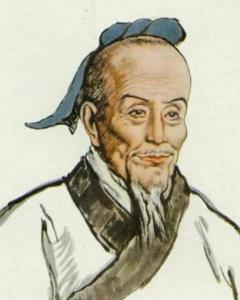
\includegraphics[scale=0.5]{img/zuchongzhi}
 \caption{何兆武以竺可桢为蓝本创作的祖冲之像}
 \label{fig:zuchongzhi}
\end{figure}

\begin{quotation}
宋末,南徐州从事史祖冲之,更开密法,以圆径一亿为一丈,圆周盈数三丈一尺四寸一分五厘九毫二秒七忽,朒数三丈一尺四寸一分五厘九毫二秒六忽,正数在盈朒二限之间。密率,圆径一百一十三,圆周三百五十五。约率,圆径七,周二十二。”
\end{quotation}

翻译为白话:南朝宋\footnote{宋武帝刘裕所创,又称“刘宋”}末年,南徐州\footnote{永嘉南渡后,汉族士大夫和侨民思念北方的故乡,就用同样的地名冠以“南”字来命名侨居地,如南徐州、南兖州、南琅琊等。}人祖冲之创立了密法,他把一丈化为一亿忽,以此为直径求圆周率。他计算的结果共得到两个数:一个是圆周率的上限(盈数)3.1415927;一个是下限(朒数)为3.1415926。人们把这一数值称做“祖率”。为了使用方便,祖冲之还给出了两个圆周率的分数值,一个是$\dfrac{355}{113}$,比较精密,称为“密率”;一个是$\dfrac{22}{7}$,称为“约率”。注意到约率和阿基米德给出的近似分数不谋而合。密率的十进制小数为$3.1415929$,误差只有$2 \times 10^{-6}$。一方面它容易记忆:只要把前三个奇数成对列出113355,然后在中间插入“分之”就得到了“113分之355”;另一方面它的精度很高,是分母在一万以内的所有分数中最接近$\pi$的(\cref{qn:113355best}要求证明这一点)。

人们猜测祖冲之的方法也是割圆术,据说他使用24576边形逼近$\pi$。但我们没有找到相关的文献实证。无论如何“祖率”的精度达到了割圆术的顶峰,祖冲之几乎给几何方法计算圆周率划上了句号,此后圆周率的计算方法就转向了无穷级数。祖冲之的心血、努力、毅力令人敬佩,是我国古代数学与科学的文化符号。据说1932年国立清华大学入学考试中有一道对联题目:上联是“孙行者”,下联答案是“祖冲之”\cite{BaiHuawen}。
%% 白化文《学习写对联》

%% 割圆术和倍边公式
接下来我们要揭开割圆术的面纱,了解古人到底是如何手工逼近圆周率的。你有没有注意到:割圆术中所有正多边形的边数都是6的倍数,并且是$2^n$次幂。例如:$96 = 2^4 \times 6$、$192 = 2^5 \times 6$,甚至传说中的$24576 = 2^{12} \times 6$。这是因为单位圆内接正六边形的周长最容易算出,6个边长为1的正三角形的底边和是6。接下来古人不断把边数加倍:$6, 12, 24, \dotsc$,每次加倍后利用勾股定理算出新的边长。如\cref{fig:double-edges}所示,过外接圆心作正多边形每一边AB的中垂线,交AB于D,交外接圆于C。连接AC、BC就实现了倍边。记原正多边形的边长为$c$,倍边后正多边形的边长为$c'$。直角三角形AOD中,斜边AO等于半径1,直角边AD是原边长的一半$\dfrac{c}{2}$,由勾股定理,另一直角边:

\begin{figure}[htbp]
 \centering
 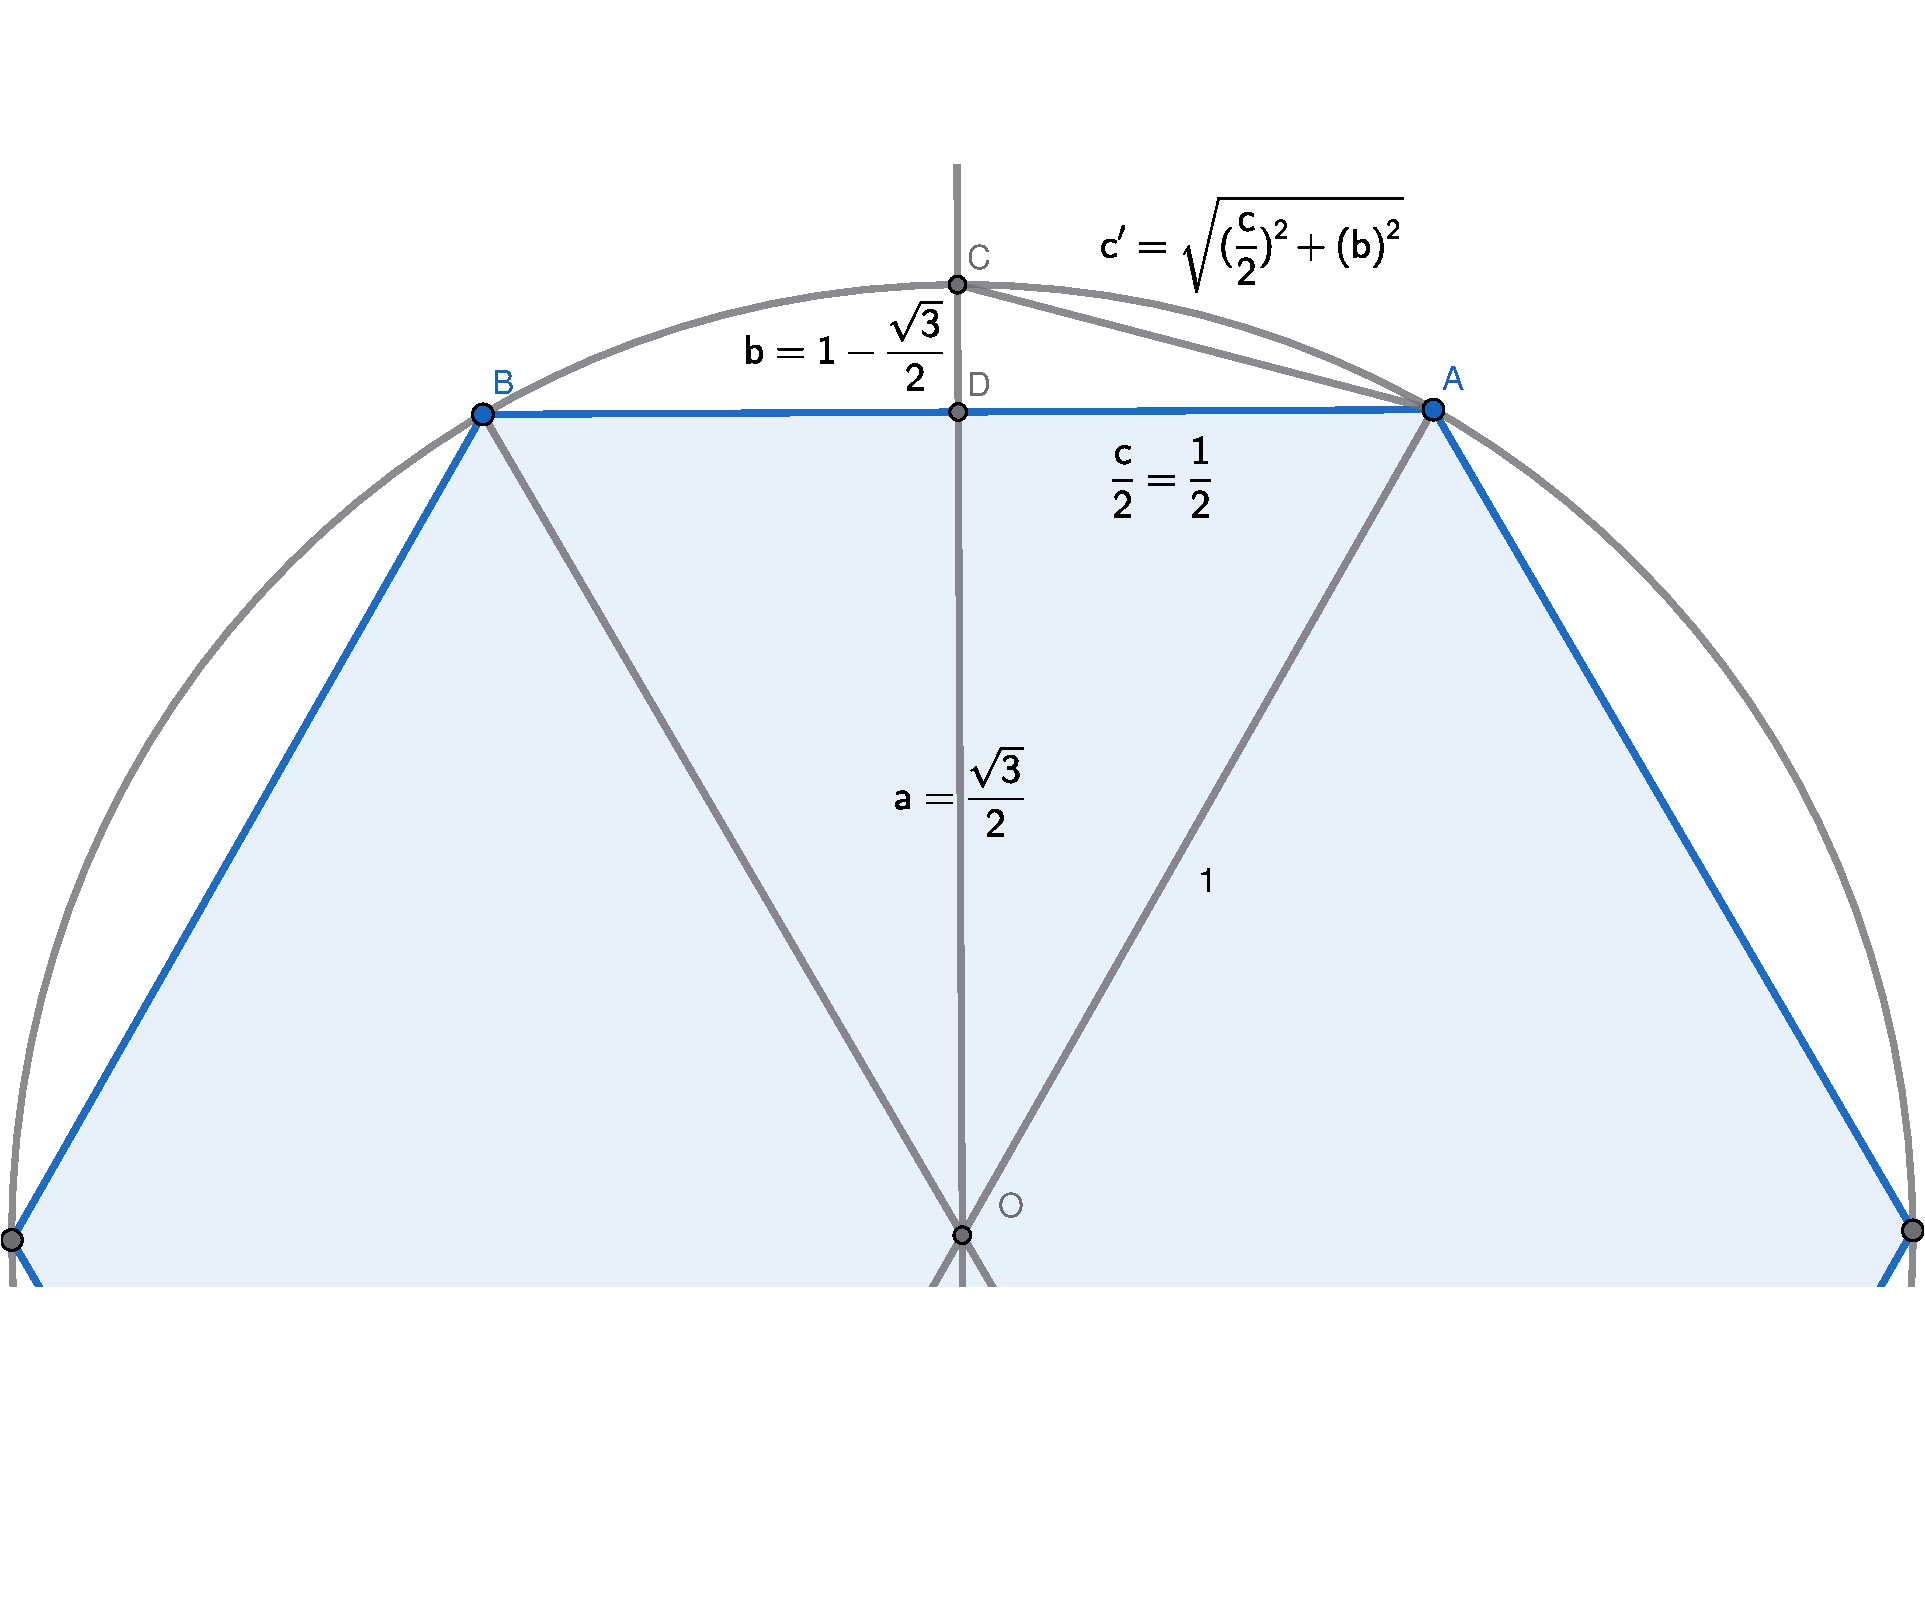
\includegraphics[scale=0.35]{img/double-edges}
 \caption{正六边形倍边}
 \label{fig:double-edges}
\end{figure}

\[
OD = \sqrt{AO^2 - OD^2} = \sqrt{1 - (\frac{c}{2})^2}
\]

在直角三角形ADC中,直角边$DC = OC - OD$。再次应用勾股定理求斜边AC:

\begin{align}
AC &= \sqrt{DC^2 + AD^2} = \sqrt{(OC - OD)^2 + (\frac{c}{2})^2}  \\
c' &= \sqrt{(1 - \sqrt{1 - (\frac{c}{2})^2})^2 + (\frac{c}{2})^2}
\label{eq:double-edges}
\end{align}

这个公式叫做“倍边公式”。如果原多边形是正六边形,$c = 1$,则倍边后正十二边形的周长是:

\[
c' = \sqrt{(1 - \sqrt{1 - (\frac{1}{2})^2})^2 + (\frac{1}{2})^2} = \sqrt{2 - \sqrt{3}}
\]

这样正十二边形的周长就是$12\sqrt{2 - \sqrt{3}}$,估计出的圆周率为$\pi > 6\sqrt{2 - \sqrt{3}}$。接下来我们还要摆上最后一块拼图:解密古人是如何手算开平方的。为了计算$\sqrt{n} = a.bcd\dotsm$,我们首先估计它的整数部分$a$。以$\sqrt{5}$为例,由$2^2 = 4 < 5 < 9 = 3^2$,估计$\sqrt{5}$的整数部分是$a = 2$,形如$2.bcd\dotsm$。接下来估计十分位小数$b$。考虑$(a + \dfrac{b}{10})^2 < n$。利用完全平方公式:

\[
(a + \frac{b}{10})^2 = a^2 + \frac{ab}{5} + \frac{b^2}{100}  < n \\
\]

以$\sqrt{5}$为例,代入$a = 2$求$b$:

\begin{align*}
4 + \frac{2b}{5} + \frac{b^2}{100} &< 5 \\
 \Rightarrow & b = 2
\end{align*}

估计出十分位$b = 2$。这样重复迭代求下一位小数$c$,由$(a + \dfrac{b}{10} + \dfrac{c}{100})^2 < n$估计出$c = 3$。不断重复直到达到所需要的精度\footnote{《九章算术》少广一章中记有古人的方法:“开方术曰:置积为实。借一算步之,超一等。议所得,以一乘所借一算为法,而以除。除已,倍法为定法。其复除。折法而下。复置借算步之如初,以复议一乘之,所得副,以加定法,以除。以所得副从定法。复除折下如前。若开之不尽者为不可开,当以面命之。若实有分者,通分内子为定实。乃开之,讫,开其母报除。若母不可开者,又以母乘定实,乃开之,讫,令如母而一。”可见古人在估算$b$时舍弃了$\frac{b^2}{100}$的项。},古人就是这样计算出$\sqrt{3} \approx 1.732$,\cref{qn:calc-sqrt3}要求手工计算$\sqrt{3}$到小数点后3位。把1.732代入倍边公式得到正十二边形的边长$c' = 0.517$,周长为6.204,估计圆周率$\pi > 3.102$。就这样古人可以继续迭代把0.517代入倍边公式,求出正24边形、48边形、96边形……的边长,乘以$n$得到周长,再除以直径估计出越来越精确的圆周率。


\subsection{无穷级数}
祖冲之的结果领先了七个世纪。直到1430年才由阿拉伯数学家阿尔·卡西(Al-Kashi)打破。出于天文学计算的需要,阿尔·卡西希望计算出宇宙的周长,并使得精度在一根头发的粗细。他认为宇宙的天球直径是地球直径的600000倍。为此他使用了$3 \times 2^{27} = 805306368$边形进行逼近。算出$\pi = 3.1415926535897932$。我们今天知道,使用39位精度的圆周率计算出可观测宇宙宇宙的直径,其误差只有氢原子半径的大小。

无穷级数法,伟达,莱布尼茨,现代方法。

pi是无理数的证明

山巅一寺一壶酒。

\section{思想之剑}
Eudoxus's theory of proportions
Dedekind cut

\begin{Exercise}[label={ex:reals}]

\Question{证明祖冲之的密率是分母在一万以内的所有分数中最接近$\pi$的。提示:利用$\pi$的连分数表示。
%% $\pi = [3;7,15,1,292,1,1,1,2,...]$
}

\Question{利用古人的方法手工计算$\sqrt{3}$到小数点后3位。\label{qn:calc-sqrt3}}
\end{Exercise}

%% ========== 答案 ====================

\begin{Answer}[ref={ex:reals}]

\Question{证明祖冲之的密率是分母在一万以内的所有分数中最接近$\pi$的。提示:利用$\pi$的连分数表示。\label{qn:113355best}
$\pi = [3;7,15,1,292,1,1,1,2,...]$
}

\Question{利用古人的方法手工计算$\sqrt{3}$到小数点后3位。}

\end{Answer}

\ifx\wholebook\relax \else
\section{参考答案}
\shipoutAnswer

\subimport{inc/}{evenpfnum-zh-cn}

\begin{thebibliography}{99}
\subimport{inc/}{bib-zh-cn}
\end{thebibliography}

\expandafter\enddocument
\fi
